\documentclass[12pt,UTF8]{ctexbook}
\usepackage{ctex}
\usepackage{array}
\usepackage{graphicx}
\usepackage{wrapfig}
\usepackage[table,dvipsnames]{xcolor}
\usepackage{tabularx}
\usepackage{longtable}
\usepackage{float}
\usepackage{amsmath}
\usepackage{amssymb}
\usepackage{xfrac}
\usepackage{eucal}
\usepackage{titlesec}
\usepackage{amsthm}
\usepackage{tikz-cd}
\usepackage{enumitem}
\usepackage{verbatim}
\usepackage{fontspec,xunicode,xltxtra}
\usepackage{xeCJK} 
\usepackage{caption}
\usepackage{thmtools, thm-restate}
% 修改脚注的编号为加圈样式,并且各页单独编号
\usepackage{pifont}
\usepackage[perpage,symbol*]{footmisc}
\DefineFNsymbols{circled}{{\ding{192}}{\ding{193}}{\ding{194}}
{\ding{195}}{\ding{196}}{\ding{197}}{\ding{198}}{\ding{199}}{\ding{200}}{\ding{201}}}
\setfnsymbol{circled}

\definecolor{gl}{RGB}{246, 252, 240}
\definecolor{gd}{RGB}{236, 244, 230}
\definecolor{bg}{RGB}{242, 244, 228}

\setCJKmainfont[BoldFont=STZhongsong]{STSong}
\setCJKmonofont{simkai.ttf} % for \texttt
\setCJKsansfont{simfang.ttf} % for \textsf
\setlength\parskip{8pt}
\setlength{\fboxsep}{12pt}
\renewcommand\thesection{\arabic{chapter}.\arabic{section}}
\newcommand{\arccot}{\operatorname{arccot}}
\newcommand{\dlim}[1]{^{\color{gray}\prime}#1}
\newcommand{\lian}[1]{
    \underset{#1}{\operatorname{lian}\,}
}
\newcommand{\di}[1]{\,\mathrm{d}#1}
% developpements limites
\newcommand{\oveq}[1]{\overset{#1}{=}} 
\newcommand{\olim}[1]{\mathit{o}\left(#1\right)}  % petit o
\newcommand{\Olim}[1]{\mathcal{O}\left(#1\right)}  % grand O
\newcommand{\Tlim}[1]{\mathcal{\Theta}\left(#1\right)}  % grand theta
\newcommand{\eqlim}[1]{\overset{#1}{\sim}}  % equivalence
\newcommand{\vect}[1]{\left\langle #1 \right\rangle}


\renewenvironment{proof}{\paragraph{\textbf{证明:}}}{\hfill$\square$}

\newtheorem{df}{定义}[section] 
\newtheorem{pp}{命题}[section]
\newtheorem{tm}{定理}[section]
\newtheorem{ex}{例子}[section]
\newtheorem{et}{例题}[section]
\newtheorem{sk}{思考}[section]
\newtheorem*{po}{公理}
\newtheorem*{so}{解答}
\newtheorem{xt}{习题}[section]
\newtheorem{cor}{推论}[pp]

% 列举环境的行间距
\setenumerate[1]{itemsep=0pt,partopsep=0pt,parsep=0pt,topsep=0pt}
\setitemize[1]{itemsep=0pt,partopsep=0pt,parsep=0pt,topsep=0pt}
\setdescription{itemsep=0pt,partopsep=0pt,parsep=0pt,topsep=0pt}
% 章节字体大小
\titleformat{\section}{\zihao{-2}\bfseries}{ \thesection }{16pt}{}
% 封面
\title{\zihao{0} \bfseries 第三册}
\author{\zihao{2} \texttt{大青花鱼}}
% \date{\bfseries\today}
\date{}
% 正文
\begin{document}
\maketitle
\tableofcontents
\newpage

\chapter{无穷}
我们已经学习过无穷的概念。我们用数数原则来判定无穷。简单来说,数得尽的集合是有穷的,数不尽的集合是无穷的。
现在,我们来进一步探讨无穷的性质。

数数原则把集合分成有穷的和无穷的两种。有穷的集合,集合元素的个数是可以知道的,
因为按照定义,它是数得尽的。

我们把有穷集合的元素个数称为\textbf{集合的势},用数字绝对值的符号来表记。
比如,空集的势就是$0$,记作$|\varnothing| = 0$。集合$\{2,5,1\}$的势是$3$,
记作$|\{2, 5, 1\}| = 3$。

比较两个集合的势,可以用最简单的“对消法”:每次从集合$A$中“拿掉”一个元素,
对应地,也从集合$B$中“拿掉”一个元素。直到某个集合的元素被“拿光”。
如果另一个集合里还有元素,就说明前者的势小于后者;如果另一个集合里也没有元素了,就说明两者的势相等。

容易验证,有穷集合的势有以下的基本性质:
\begin{enumerate}
    \item 子集的势不多于母集的势;真子集的势小于真母集的势。
    \item 集合$A$在集合$B$中补集的势,加上$A$的势,等于$B$的势。
\end{enumerate}

\section{无穷集合的势}

有穷集合的基本性质符合我们日常生活中的经验。对于无穷集合,它们是否也成立呢?

来看以下的例子。

一个旅馆里有无穷个房间。房间的号码是正整数:$1$号、$2$号、$3$号……

一天,有一个客人来旅馆里住宿。可所有的房间都住了人,怎么办呢?
旅馆的老板说:这样吧,我们把$1$号房的客人转到$2$号房,把$2$号房的客人转到$3$号房,
把$3$号房的客人转到$4$号房……以此类推,$n$号房的人转到$n+1$号房。

这样,$1$号房就空出来了。客人顺利入住。

又一天,有无穷多个客人来旅馆里住宿。可所有的房间都住了人,怎么办呢?
旅馆的老板一看,每个客人有一个正整数号码,没有重复的也没有缺少的,恰好和房号一样。
老板说:这样吧,我们把$1$号房的客人转到$2$号房,把$2$号房的客人转到$4$号房,
把$3$号房的客人转到$6$号房……以此类推,$n$号房的人转到$2n$号房。

这样,所有奇数号的房间就空出来了。于是,$1$号客人住$1$号房,$2$号客人住$3$号房,$3$号客人住$5$号房,……以此类推,
$n$号客人入住$2n-1$号房。这样,所有的客人都顺利入住了。

以上的情况似乎有点违反我们的直觉。集合$\{2,3,4,\cdots\}$和$\{2,4,6,\cdots\}$是$\{1,2,3,\cdots\}$的真子集,
但它们的势与$\{1,2,3,\cdots\}$相等。这说明,无穷集合的势,有着不同的性质。

为此,我们首先要定义无穷集合的势的关系。我们从“对消法”出发来构思。
“对消法”中,我们实际上在给两个集合的元素建立一一对应的关系。
每次从两个集合里分别“拿掉”的元素形成一一对应。

如果一个集合“拿光”的时候,另一个集合也“拿光”了,
说明我们给两个集合的元素建立了一一对应的映射,也就是双射。

如果一个集合“拿光”的时候,另一个集合还有“剩余”,就说明我们无法在两个集合的元素之间建立双射。
我们可以从前一个集合出发,建立到后一个集合的单射;但无法从后一个集合出发,建立到前一个集合的单射。
这是因为后一个集合的元素太多了,总会有两个元素映射到同一个目标。

用这个思路,我们来定义无穷集合的势的关系。

\begin{df}\label{df:1-0-0}
    设有集合$A$和$B$。
    \begin{itemize}
        \item 如果存在$A$到$B$的双射,就说$A$和$B$的势相等,两者等势,记作$|A| = |B|$。
        \item 如果存在从$A$到$B$的单射,就说$A$的势不大于$B$的势或$A$的势小于等于$B$的势,记作$|A| \leqslant |B|$或$|B| \geqslant |A|$。
        \item 如果存在从$A$到$B$的单射,但不存在$B$到$A$的单射,就说$A$的势小于$B$的势,记作$|A| < |B|$或$|B| > |A|$。
    \end{itemize}
\end{df}

用这个定义,就可以理解无穷旅馆的例子。对于集合$\{1,2,3,\cdots\}$和$\{2,3,4,\cdots\}$来说,
我们有双射$n\mapsto n+1$,因此两者等势。
对于集合$\{1,2,3,\cdots\}$和$\{2,4,6,\cdots\}$来说,我们有双射$n\mapsto 2n$,因此两者等势。

注意:
\begin{enumerate}
    \item 以上定义对有穷集合、无穷集合都成立,也就是说,上面的$A$、$B$分别可以是有穷、无穷集合。
    \item 对于有穷集合$A$、$B$,这个定义与有穷集合的势的定义是兼容的。
    \item \textbf{无穷集合的势不是数}。我们沿用有穷集合的记法,把无穷集合$A$的势记作$|A|$。
    但$|A|$并不是任何数。因此,\textbf{无穷集合的势不能参与四则运算}。
    \item 同样地,当我们写$|A| \leqslant |B|$、$|A| = |B|$的时候,
    里面的等号和不等号也不能按数的相等、不等关系来理解。但在一定条件下,它们的性质和数的相等、不等关系是一样的(具体参见附录$A$)。
\end{enumerate}

\begin{sk}
    \mbox{} \\
    \indent 1. 在无穷旅馆的例子里,如果旅馆已经住满了,而有无穷多个旅客来住宿,
    旅客的编号用全体整数来编号。是否能腾出足够的房间呢?如何操作?如果旅客的编号用全体有理数呢?全体实数呢?\\
    \indent 2. 请用满射代替单射,定义无穷集合的势的关系。\\
    \indent 3. 能否给无穷集合的势定义四则运算?
\end{sk}


\begin{xt}
    \mbox{} \\
    \indent 1. 以下集合的势是多少?
    $$ 
    \begin{array}{l}
        1.\,1. \,\,\,\{\mbox{一年中的月份}\} \\
        1.\,2. \,\,\,\{100\mbox{以内的素数}\}\\
        1.\,3. \,\,\,\{S\mbox{的所有子集}\}\mbox{,其中}|S| = 9. \\
        1.\,4. \,\,\,\{(x, \,\, y, \,\, z) \, | \, 0 \leqslant x, y, z \leqslant 3, x + 2y + z \leqslant 8,\,\,\, x,\,\, y \in  \mathbb{Z}\}
    \end{array}
    $$
    \indent 2. 证明:把有穷集合的势定义为元素的个数,这样的定义,满足定义\ref{df:1-0-0} 中势的关系。\\
    \indent 3. 证明:有穷集合的势总小于无穷集合的势。\\
    \indent 4. 证明,如果集合$A$是$B$的子集,那么$|A| \leqslant |B|$。\\
    \indent 5. 证明:定义\ref{df:1-0-0} 中集合的势相等的关系,是一种等价关系,即满足:
    \indent \begin{itemize}
        \item 自返性:任意集合$A$的势等于自己:$|A| = |A|$。
        \item 对称性:若集合$A$的势等于集合$B$的势,则集合$B$的势等于集合$A$的势。
        \item 传递性:若集合$A$的势等于集合$B$的势,集合$B$的势等于集合$C$的势,则集合$A$的势等于集合$C$的势。
    \end{itemize}

    \indent 6. 证明:如果集合$A$、$B$满足$|A| < |B|$,那么$|A| = |B|$不成立。

    % \indent 6. 证明:定义\ref{df:1-0-0} 中集合的势小于等于的关系满足:\\
    % \indent \begin{itemize}
    %     \item 自返性:任意集合$A$的势等于自己:$|A| = |A|$。
    %     \item 对称性:任何集合$A$、$B$,$|A| \leqslant |B|$和$|B| \leqslant |A|$至少有一个成立。
    %     \item 传递性:若集合$A$的势小于等于集合$B$的势,集合$B$的势小于等于集合$C$的势,则集合$A$的势小于等于集合$C$的势。
    % \end{itemize}

    % \indent 7. 证明:定义\ref{df:1-0-0} 中集合的势小于的关系满足:
    % \indent \begin{itemize}
    %     \item 自背性:任意集合$A$的势不小于自己:$|A| < |A|$总不成立。
    %     \item 三分律:任何集合$A$、$B$的势总恰好满足$|A| < |B|$、$|A| = |B|$、$\qquad |B| < |A|$之一。
    %     \item 传递性:若集合$A$的势小于集合$B$的势,集合$B$的势小于集合$C$的势,则集合$A$的势小于集合$C$的势。
    % \end{itemize}
    
    
\end{xt}

\section{常见无穷集合的势}

常见的无穷集合有:自然数集$\mathbb{N}$、正整数集$\mathbb{Z}^+$、整数集$\mathbb{Z}$、
有理数集$\mathbb{Q}$、实数集$\mathbb{R}$等等。下面来看一些无穷集合的势的关系。

容易看出,$|\mathbb{N}| = |\mathbb{Z}^+|$,两者间的关系可以用双射$n\mapsto n + 1$确立。
而双射$n \mapsto -n$可以说明$|\mathbb{Z}^+| = |\mathbb{Z}^-|$,所以$|\mathbb{N}| = |\mathbb{Z}^-|$。

考虑把整数映射到自然数的映射:
$$ f,\,\,\,n\mapsto \left\{
    \begin{array}{cl}
        2n & \mbox{如果}n \geqslant 0 \\
        -2n - 1  & \mbox{如果}n < 0 
    \end{array}\right.
$$
也就是:
$$ \begin{array}{cccccccc}
        0 & -1 & 1 & -2 & 2 & -3 & 3 & \cdots \\
        \downarrow & \,\downarrow & \downarrow & \,\downarrow & \downarrow & \,\downarrow & \downarrow & \cdots \\
        0 & \,1 & 2 & \,3 & 4 & \,5 & 6 & \cdots 
    \end{array}
$$
它把所有自然数对应到自然数中的偶数,把所有负整数对应到自然数中的奇数。

不难验证,映射$f$是单射。
这是因为,给定两个不相同的正数$m \neq n$,如果两者一个小于零,一个不小于零,那么两者映射的结果奇偶性不同,因此不相等;
如果两者同时小于零或同时不小于零,按定义$2m \neq 2n$、$-2m - 1 \neq -2n - 1$,也就是说两者映射的结果不相等。
综上所述,如果$m \neq n$,那么$f(m) \neq f(n)$。

同时,映射$f$也是满射,因为任何偶数$n$都是整数$\frac{n}{2}$映射的结果,任何奇数$n$都是整数$-\frac{n+1}{2}$映射的结果。

$f$既是单射也是满射,因此是双射。我们在自然数集$\mathbb{N}$和整数集$\mathbb{Z}$之间建立了双射$f$,
这说明$|\mathbb{N}| = |\mathbb{Z}|$。

考虑平面所有坐标是自然数的点的集合:$\mathbb{N}^2 = \{(x,\,\,y) \, | \, x, \,\, y \in \,\, \mathbb{N}\}$。
$\mathbb{N}^2$的势与$\mathbb{N}$的势关系如何呢?

我们希望找出一种按顺序数出$\mathbb{N}^2$中所有点的数数方法。
这样,我们就可以把$1$映射到数数中的第一个点,把$2$映射到数数中的第二个点,等等,
建立从$\mathbb{Z}^+$到$\mathbb{N}^2$的映射。这个映射如果是双射,那么$\mathbb{N}^2$的势就等于$\mathbb{Z}^+$的势,从而等于$\mathbb{N}$的势。

考虑这样的数数方法:把点的横坐标和纵坐标加起来。从和最小的点开始数起,逐步增大。
对于和相等的点,则按照横坐标,从小数到大。
也就是按照图中箭头的方法来数数。这样的数法,可以不重复不遗漏地数遍$\mathbb{N}^2$所有的点。

\begin{figure}[h] %this figure will be at the right
    \vspace{4pt}
    \centering
    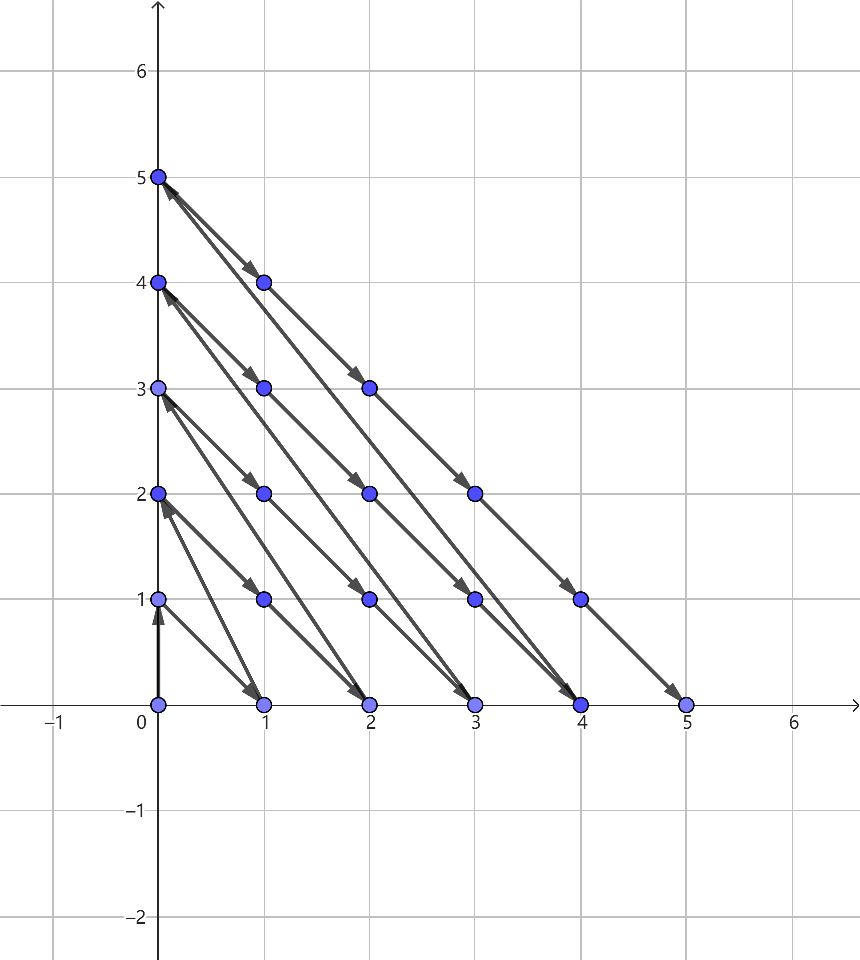
\includegraphics[width=0.4\textwidth]{tu/无穷1.png}
    \caption*{\texttt{按照箭头方向,可以不重复不遗漏数遍}$\mathbb{N}^2$\texttt{中所有的点}}
\end{figure}

相应地,把正整数$n$映射到这个数法的第$n$个点,这样的映射就是双射。因此,按前面的推理,我们得到结论:
$$ |\mathbb{N}^2| = |\mathbb{N}|.$$

类似地,考虑正有理数集$\mathbb{Q}^+$。对有理数$r$,将它写成既约分数$\frac{p}{q}$,考虑分子分母之和。
从和最小的开始数起,逐步增加。如果某些有理数按以上方法得到的和相等,这样的有理数个数有限,把它们按分子从小到大排列,从分子最小的数起。
这样,我们得到了一种不重复不遗漏数遍所有正有理数的方法:
$$ \frac{1}{1} \rightarrow \frac{1}{2} \rightarrow \frac{2}{1} \rightarrow \frac{1}{3} \rightarrow \frac{3}{1} \rightarrow \frac{1}{4} \rightarrow \frac{2}{3} \rightarrow \frac{3}{2} \rightarrow \frac{4}{1} \rightarrow \cdots$$
这表明$\mathbb{Q}^+$的势等于$\mathbb{Z}^+$的势,从而等于$\mathbb{N}$的势。
$$ |\mathbb{Q}^+| = |\mathbb{N}|.$$

我们考虑把$\mathbb{N}$映射到$\mathbb{Q}^+$的双射$f$。考虑以下映射:
$$ g:\,\,\,r\mapsto \left\{
    \begin{array}{cl}
        0 & \mbox{如果}r = 0 \\
        f(r) & \mbox{如果}r > 0 \\
        -f(-r)  & \mbox{如果}r < 0 
    \end{array}\right.
$$
$g$把所有整数映射为有理数。由于$f$是双射,容易证明$g$也是双射。因此我们有$\mathbb{Z}$到$\mathbb{Q}$的双射,
这说明$\mathbb{Q}$的势等于$\mathbb{Z}$的势,从而等于$\mathbb{N}$的势。
$$ |\mathbb{Q}| = |\mathbb{N}|.$$

% \begin{sk}
%     \mbox{} \\
%     \indent 1. 
% \end{sk}


\begin{xt}
    \mbox{} \\
    \indent 1. 给定数集$A$和正整数$k\geqslant 2$,定义由$k$个$A$中元素构成的有序数组的集合为:
    $$ A^k = \{(a_1, a_2, \cdots, a_k) \, | \, a_1, a_2, \cdots, a_k \,\, \in A \}.$$
    \indent 1.1. 考虑$A = \mathbb{N}$的情况。考虑$\mathbb{N}^k$中的有序数组$(a_1, a_2, \cdots, a_k)$中的$k$个数的和。
    记所有和等于自然数$p$的有序数组构成的集合为$S_p$。证明:所有的$S_p$构成$\mathbb{N}^k$的分划。\\
    \indent 1.2. 给定正整数$k\geqslant 2$,考虑$\mathbb{N}^{k+1}$和$\mathbb{N}^{k}$按上一问构成的分划。
    如果$|\mathbb{N}^k| = |\mathbb{N}|$,证明:可以给出一种不重复不遗漏数遍$\mathbb{N}^{k+1}$的方法。\\
    \indent 1.3. 用归纳法证明:对任何正整数$k\geqslant 2$,$|\mathbb{N}^k| = |\mathbb{N}|$。\\
    \indent 1.4. 证明:$|\mathbb{Z}^k| = |\mathbb{N}|$。\\
    \indent 2. 证明:$\mathbb{N}$的子集要么有限,要么和$\mathbb{N}$等势。\\
    \indent 3. 证明:如果$|A| = |B| = |\mathbb{N}|$,那么$|A\cup B| = |\mathbb{N}|$。
\end{xt}

\section{可数和不可数}
上一节中,我们研究了一些常见数集的势。很多直观上似乎比自然数集“大得多”的数集,都和自然数集等势。
那么,是否有比自然数集“大”的数集呢?

考虑数列的项只有$0$和$1$的数列。我们把所有这样的数列构成的集合记为$2^\mathbb{N}$:
$$ 2^\mathbb{N} = \left\{\left\{a_n\right\}_{n\in\mathbb{N}} \, | \, \forall n\in\mathbb{N}, a_n \in \{0, 1\} \right\}. $$
下面我们证明:
$$|\mathbb{N}| < |2^\mathbb{N}|$$
也就是说,存在$\mathbb{N}$到$2^\mathbb{N}$的单射,但不存在$2^\mathbb{N}$到$\mathbb{N}$的单射。

首先考虑映射:
$$ \forall n\in\mathbb{N}, \quad n \mapsto \left\{a_k\right\}_{k\in\mathbb{N}}, \,\,\, \mbox{其中} \, a_k = 1 \,\mbox{当且仅当} \, k = n . $$
这个映射显然是单射,因此存在$\mathbb{N}$到$2^\mathbb{N}$的单射。

如何证明不存在$2^\mathbb{N}$到$\mathbb{N}$的单射呢?我们用反证法证明。

假设存在$2^\mathbb{N}$到$\mathbb{N}$的单射$f$,则$2^\mathbb{N}$所有元素经过映射得到的集合是$\mathbb{N}$的无穷子集,因而和$\mathbb{N}$等势。
也就是说,我们可以假设$f$是满射,因而是双射。因此,我们考虑它的逆映射$g$。$g$是把自然数映射到$2^\mathbb{N}$中元素的双射。
因此,我们可以把$2^\mathbb{N}$中的元素按数数的方式列出来:
\begin{align*}
    0 &\mapsto a_{0,0}, a_{0,1}, a_{0,2}, \cdots , a_{0,k}, \cdots  \\
    1 &\mapsto a_{1,0}, a_{1,1}, a_{1,2}, \cdots , a_{1,k}, \cdots  \\
    2 &\mapsto a_{2,0}, a_{2,1}, a_{2,2}, \cdots , a_{2,k}, \cdots  \\
    \vdots & \qquad \qquad\qquad \vdots  \\
    n &\mapsto a_{n,0}, a_{n,1}, a_{n,2}, \cdots , a_{n,k}, \cdots  \\
    \vdots & \qquad \qquad\qquad \vdots  
\end{align*}
其中$a_{n,k}$是$n$对应的数列中的第$k$项。现在考虑这么一个数列$W$:
它的第$k$项就是$1$减去上面排列中$k$对应的数列的第$k$项。
也就是说,如果该项是$0$,$W$的第$k$项就是$1$,如果该项是$1$,$W$的第$k$项就是$0$。
按定义,$W$的第$k$项一定不等于上面排列中第$k$行数列的第$k$项。

按照$g$的定义,$W$肯定是某个自然数$m$经过$g$得到的结果,因此,它排在上面排列中的第$m$行。
但是,它的第$m$项就是$a_{m,m}$。然而按照$W$的定义,它的第$m$项应该是$1 - a_{m,m}$,不等于$a_{m,m}$。
这就构成了矛盾。

因此,不存在$\mathbb{N}$到$2^\mathbb{N}$的单射。

这样,我们得到了一个严格“大于”自然数集的集合。

以上结果说明:即便是无穷集合,也有“大小之分”。为此,我们要给无穷集合做更精细的划分。
注意到以上证明里,我们通过把$2^\mathbb{N}$中的元素用数数的方式列出来,而导出了矛盾。
这个矛盾说明了$2^\mathbb{N}$这样的集合的本质:它是“不可数”的。

我们把自然数集这样可以用数数的方式列出来的集合(也就是与$\mathbb{N}$等势的集合)
称为\textbf{可数集合}或\textbf{可列集合},
而把$2^\mathbb{N}$这样的集合称为\textbf{不可数集合}或\textbf{不可列集合}。
而以上的推理说明,\textbf{不可数集合总大于可数集合}。

不可数集合是否也有类似无限旅馆这样的现象呢?

对于可数集合,它的子集如果是无限的,就和它等势。
换句话说,如果从可数集合中去掉有限个元素,得到的子集和它等势。
用不严谨的话来说,这是由于有限集合相比可数集合是“非常小”的,是可以忽略的。

这个关系在可数集合与不可数集合之间也有体现。

\begin{tm}
    设$S$是不可数集合,它的子集$A$是可数集合,则$S$去除$A$中元素得到的集合$S\backslash A$与$S$等势。
\end{tm}

\begin{proof}
    首先用反证法证明$S\backslash A$是不可数集合。$S$是$A$与$S\backslash A$的并集。
    如果$A$和$S\backslash A$都是可数集合,那么它们的并集$S$也是可数集合。矛盾!

    接下来证明$|S\backslash A| = |S|$。考虑$S\backslash A$的可数子集$B$,记$S\backslash A$去掉$B$中元素得到的集合为$C$,
    则$A$、$B$、$C$是$S$的分划,$S = A\cup B\cup C$。
    
    注意到由于$S\backslash A$是不可数集合,$B$是可数集合,所以$C$也是不可数集合。
    另外,由于$A$、$B$是可数集合,所以$ |A| = |B| = |\mathbb{N}|$,于是$|A\cup B| = |\mathbf{N}|$。
    因此,存在从$B$到$A\cup B$的双射$g$。

    考虑映射:
    $$ f:\,\,\,x\mapsto \left\{
        \begin{array}{cl}
            g(x) & \mbox{如果}x\in B \\
            x & \mbox{如果}x \in C
        \end{array}\right.
    $$
    则$f$是$S\backslash A$到$S$的双射。因此$|S\backslash A| = |S|$。
    
\end{proof}

这说明,可数集合比起不可数集合,就和有限集合相比可数集合一样,是可以忽略的。

最后来看实数集$\mathbb{R}$。它是否可数呢?我们可以用证明$2^\mathbb{N}$类似的想法。

给定实数$x$,我们可以将它写成小数的形式。如果$x$是有穷小数,就在最后补上无穷多个$0$。
这样,每个实数都可以写成无穷小数。也就是说,我们可以把每个实数对应到类似$0$到$9$组成的无穷数列。

假设实数集可数,那么可以像前面的证明里那样,构造正整数集到实数集的双射,把所有实数依次排列出来。
各个实数的小数部分就和$2^\mathbb{N}$里的数列一样。于是,我们构造这样的实数$a$,
它的小数部分第$k$位数字和排第$k$位的实数的小数部分第$k$位数字不一样。
但另一方面,$a$也是某个正整数$m$映射的结果。因此按照定义,$a$的小数部分第$m$位不能等于自己。矛盾!
因此我们可以得出结论:实数集不可数。

实际上,我们可以严谨证明:实数集$\mathbb{R}$和$2^\mathbb{N}$等势,具体参见附录$A$。

研究了常见的无穷数集的势,我们发现,目前我们所知的无穷集合有两类。
一类数集与自然数集$\mathbb{N}$等势,是为可数集合。另一类与实数集$\mathbb{R}$等势,等于$2^\mathbb{N}$。
那么,是否有既不等势于$\mathbb{N}$,也不等势于$2^\mathbb{N}$的无穷集合呢?

数学研究者对无穷集合的研究发现:比$2^\mathbb{N}$“更大”的无穷集合是存在的。
我们把这些类别按从小到大的顺序,记为$\aleph_0$、$\aleph_1$、$\aleph_2$、$\aleph_3$等等。
$\aleph_0$就是自然数集$\mathbb{N}$,$\aleph_1$是$2^\mathbb{N}$。
$\aleph_2$、$\aleph_3$等则是比$2^\mathbb{N}$更大的集合。

另一方面,是否存在介于$\mathbb{N}$和$2^\mathbb{N}$之间的无穷集合,则是困难得多的问题。
由于实数集是连续的,我们把这个问题称为“连续统问题”或“连续统假设”。
对这个问题的研究直接引发了对数学基本推理框架的质疑。

1963年,数学家证明了:在我们常见的推理框架内,“连续统问题”是“独立的”,
既不可能证明它成立,也不可能证明它不成立。
从另一个角度来说,不论“存在介于$\mathbb{N}$和$2^\mathbb{N}$之间的无穷集合”还是
“不存在介于$\mathbb{N}$和$2^\mathbb{N}$之间的无穷集合”,都不会导致矛盾。

\begin{xt}
    \mbox{} \\
    \indent 1. 证明:可数集合去除有限个元素后仍然是可数集合。\\
    \indent 2. 证明:无理数集是不可数集合。\\
    \indent 3. 证明:可数个两两不相交的有限集合:$\{A_n\}_{n\in\mathbb{N}}$的并集是可数集合。\\
    \indent 4. 证明:有限个可数集合的并集是可数集合;可数个可数集合的并集是可数集合;不可数集合的并集是不可数集合。
\end{xt}

\chapter{连续函数的变化}

日常生活、工程和科学研究中,我们关心事物的运动和变化。
描述、衡量、分析事物的运动和变化,是人类了解世界、科学进步的关键。
17世纪,科学研究者发现了物体受力与运动变化的关系,建立了统一的力学理论,引发了工业革命。
20世纪初,科学研究者提出了“光速不变”的假设,在此基础上构建了相对论。
这些革命性的进步,都离不开对运动本质的探索。
而对运动的深入研究,也促使了数学的发展。

数学中,我们用实变映射描述事物的运动和变化。
具体来说,我们需要研究的事物性质一些基本要素相关。
这些基本要素,比如时间、物体的位置、温度等等,我们认为是连续变化的,称为变量,用实数表示。
于是,事物的性质就是关于这些变量的映射。
分析这些映射的性质,找到适合描述实验数据的映射,是科学研究的重要部分。

\section{函数在一点的变化}
% 介绍连续函数在一点的微变率:微变率是变化率的极限
我们已经学习过用数学描述运动和变化。对于物体的运动,我们定义了平均速度,描述运动的快慢。
一般来说,我们使用变率来描述事物变化的快慢。
\begin{df}{\textbf{实变映射的变率}}
    设$f$是定义在实数集上的映射,给定实数$t_1 < t_2$,则$f$在$[t_1;t_2]$上的\textbf{变率}是:
    $$ \frac{f(t_2) - f(t_1)}{t_2 - t_1}.$$
\end{df}

平均速度就是位移函数的变率。

使用平均速度,我们可以近似描述物体位置在一段时间里的变化。
如果把物体的运动看作关于时间$t$的函数,设物体的位移为函数$p(t)$,那么,在$(t_1; t_2)$的时间段里,
物体的位移大致是:
$$ p(t) \approx p(t_1) + \frac{p(t_2) - p(t_1)}{t_2 - t_1}(t - t_1).$$
这里我们用一次函数代替了真实的位移函数$p$。直观上,在区间$(t_1; t_2)$里,
我们用直线近似表示了函数$p(t)$的图像。

很多时候,我们希望对事物的变化有更好的理解。
比如,我们可以测量一秒内物体的位移,作为平均速度。但我们还想知道,如果把一秒换成更短的$0.1$秒、$0.01$秒,
得到的结果会不会完全不同。
此外,我们可以记录运动物体在某个时刻的位移,但也希望能记录物体在该时刻的速度(或者其他变化),
以更好地理解运动的性质。
甚至,我们发现物体受到的力与物体运动速度的变率相关,也就是说,和物体位移的变率的变率相关。
这时候,我们希望能更精确地知道物体运动速度的性质,以研究它的变率。
总之,我们需要一个刻画物体在某个时刻“附近”变化快慢的量。

实践中,我们发现,对于大多数的运动物体,如果在同样条件下重复测量平均速度,
那么随着取的时间间隔越来越短,测得的平均速度会趋于某个固定的值。这个现象让我们想到函数(在一点)的极限。
因此,我们用极限的概念来描述物体某个时刻“附近”变化的快慢。

我们可以定义物体在某个时刻$t_0$的瞬时速度$v(t_0)$:
$$ v(t_0) = \lian{t\to t_0} \frac{p(t) - p(t_0)}{t - t_0}.$$
它是$t$附近的平均速度的极限。正如数列的极限不一定等于数列自身的项,瞬时速度作为变率的极限,
描述了物体在该时刻运动的快慢,但它并非变率,也不是运动。

对于一般的函数,我们也可以用这个方法描述它在一点变化的快慢。

\begin{df}\label{df:2-1-0}
给定在某一点$a$附近有定义的函数$f$,如果当$x$趋于$a$时,
$f$在$a$到$x$的变率收敛到某个极限,就说函数$f$在$a$处\textbf{可微}。
我们把这个极限叫做函数$f$在点$a$处的\textbf{微变率},简称\textbf{微变},
记作$\partial f(a)$\footnote{函数$f$在点$a$处的微变率,一般记作$\partial f(a)$或$f'(a)$,在物理书籍中也常记作$\dot{f}(a)$。
关于微变率的记法,可见附录$B$。}。
$$ \partial f(a) = \lian{x\to a} \frac{f(x) - f(a)}{x - a} = \lian{h\to 0} \frac{f(a + h) - f(a)}{h}.$$
\end{df}

比如,运动物体在某时刻的瞬时速度,就是它的位移函数在该时刻的微变率。
$$ v(t_0) = \partial p(t_0).$$

\begin{figure}[h]
    \vspace{4pt}
    \centering
    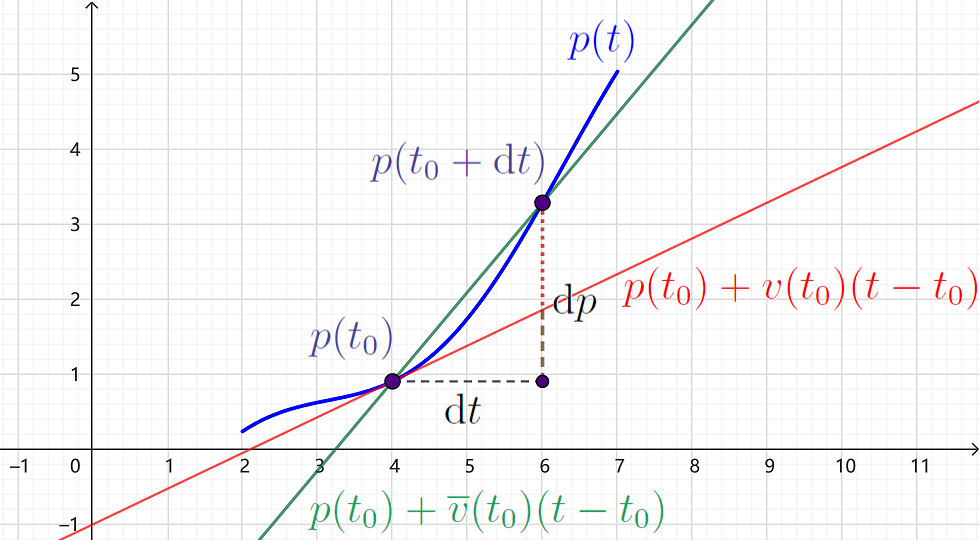
\includegraphics[width=0.7\textwidth]{tu/导数1.png}
\end{figure}

如何理解瞬时速度呢?上图是物体做直线运动时,位移关于时间的函数的图像。横坐标表示时间$t$,
纵坐标表示物体的位移$p$。我们希望了解物体在$t_0$时刻“附近”的运动情况。

从$t_0$时刻起,经过固定时段$\mathrm{d}t$,
物体的位移产生了变化:
$$\mathrm{d}p = p(t_0 + \mathrm{d}t) - p(t_0).$$
因此,这段时间内的平均速度$\overline{v}(t_0)$就是$\mathrm{d}p$与$\mathrm{d}t$的比值:
$$\overline{v}(t_0) = \frac{\mathrm{d}p}{\mathrm{d}t}.$$
从图像来看,它是过函数两点构成的绿色直线的斜率。

使用平均速度,我们可以认为,在$t_0$附近,物体大致在做速度为$\overline{v}(t_0)$的匀速运动,
位移可以用一次函数近似表示:
$$ p(t) \approx p(t_0) + \overline{v}(t_0)(t - t_0)$$
直观来说,图中函数$p(t)$的图像曲线,在$t_0$附近,可以用绿色直线近似表示。

但是,要注意的是,平均速度$\overline{v}(t_0)$不仅仅与$t_0$相关。
对不同的$\mathrm{d}t$,$\overline{v}(t_0)$是不同的。而瞬时速度$v(t_0)$的存在告诉我们,
$\overline{v}(t_0)$会随着$\mathrm{d}t$缩小而收敛。
也就是说,绿色直线会逐渐收拢到过点$(t_0, \,\,p(t_0))$、以$v(t_0)$为斜率的红色直线。
我们称这条直线为函数图像在$t_0$的\textbf{切线}。

使用瞬时速度$v(t_0)$来近似描述$t_0$附近的运动,物体的位移可以用一次函数近似表示:
$$ p(t) \approx p(t_0) + v(t_0)(t - t_0).$$

这样的表示和之前有什么不同呢?

首先,我们注意到,瞬时速度$v(t_0)$只与$t_0$相关,不需要用别的时刻$t$来计算。
其次,我们可以证明,如果要用一次函数(也就是匀速运动)来近似表示物体在$t_0$附近的运动,
瞬时速度$v(t_0)$是“最好”的系数。

直观来说,如果用一条过$(t_0, \,\,p(t_0))$点的直线近似表示物体位移的曲线,
那么对于$t_0$附近的情况,斜率为$v(t_0)$的直线是“最好”的。

为什么这么说呢?

假设我们用某个数$u$做系数,用这样的一次函数:
$$ t \mapsto p(t_0) + u\cdot (t - t_0).$$
来近似表示物体的位移。考虑$t_0$附近的$t$,实际的位移是$p(t)$,近似的位移是$p(t_0) + u(t - t_0)$。
因此近似误差为:
$$ d(t) = \left|p(t) - p(t_0) - u(t - t_0)\right|. $$
这是一个关于$t$的函数。$t$趋于$0$时,$d(t)$趋于$0$。

让我们来研究它趋于$0$有多快。我们这样来衡量:以$t\mapsto t - t_0$为参照物,考虑$d(t)$和$|t - t_0|$的比值:
$$ \frac{d(t)}{|t - t_0|} = \left|\frac{p(t) - p(t_0) - u(t - t_0)}{t -  t_0}\right| =  \left|\frac{p(t) - p(t_0)}{t -  t_0} - u\right|. $$
如果这个比值在$t$趋于$t_0$的时候的极限是$0$,就说明只要$t$与$t_0$足够近,
近似误差$d(t)$就可以比$t-t_0$小得多。这就是说$d(t)$比$t-t_0$收敛得更快。
如果比值不趋于$0$,就说明$d(t)$并不比$t-t_0$收敛得更快。

考虑这个比值在$t$趋于$t_0$时的极限:
$$ \lian{t\to t_0} \frac{d(t)}{|t - t_0|} = \left|\lian{t\to t_0} \frac{p(t) - p(t_0)}{t -  t_0} - u\right| = |v(t_0) - u|. $$
因此,这个比值趋于$0$,当且仅当$v$等于瞬时速度$v(t_0)$。

换句话说,当且仅当$u = v(t_0)$时,近似误差$d(t)$比$t-t_0$收敛得更快。只要$t$与$t_0$足够近,
近似误差就可以比$t-t_0$小得多。而$v$取其他值的时候,就没有这样的效果,近似误差至多和$t-t_0$收敛得一样快。
也就是说,$u = v(t_0)$时,近似效果是最好的。
在$t_0$附近,用微变率作为系数的一次函数和原来的函数最像。
比如,我们取$t_0$处的瞬时速度$v(t_0)$作为$t_0$附近的“平均速度”,
就比取其他的平均速度更能表现$t_0$附近的运动。

一般来说,用微变率作为系数的一次函数:
$$ t \mapsto f(t_0) + \partial f(t_0) \cdot(t - t_0)$$
称为函数$f$在$t_0$处的\textbf{微直观}。
直观上,微直观就是函数$f$在$t_0$处的切线,是$t_0$附近模拟$f$图像曲线的最佳直线。

最后来看如何具体计算微变率。

从最简单的函数出发。
常函数$x \mapsto c$在任意点的微变都是$0$。
恒等函数$x\mapsto x$在任意点的微变都是$1$。
正比例函数$x \mapsto c x$在任意点的微变都是系数$c$。以上的结论就由读者来证明。

对于稍微复杂一点的函数,我们一起来算一算。

\begin{et}
    \mbox{} \\
    \indent 1. 求函数$f: \,\, x \mapsto x^2$在点$x = 3$处的微变率。\\
    \indent 2. 求函数$f: \,\, x \mapsto \frac{1}{x}$在点$x = 2$处的微变率。\\
    \indent 3. 求函数$f: \,\, x \mapsto (x - 1)^3$在点$x = 1$处的微变率。
\end{et}

\begin{so}
    \mbox{} \\
    \indent 1. 按定义,$f$在点$x = 3$处的微变率为:
    \begin{align*}
        \partial f(3) &= \lian{h\to 0}\frac{f(3 + h) - f(3)}{h}  \\
        &= \lian{h\to 0}\frac{(3 + h)^2 - 3^2}{h}  \\
        &= \lian{h\to 0}\frac{6h + h^2}{h}  \\
        &= \lian{h\to 0}(6 + h)  \\
        &= 6.  
    \end{align*}

    \indent 2. 按定义,$f$在点$x = 2$处的微变率为:
    \begin{align*}
        \partial f(2) &= \lian{h\to 0}\frac{f(2 + h) - f(2)}{h}  \\
        &= \lian{h\to 0}\frac{\frac{1}{2+h} - \frac{1}{2}}{h}  \\
        &= \lian{h\to 0}\frac{\frac{2 - (2 + h)}{2(2 + h)}}{h}  \\
        &= \lian{h\to 0}-\frac{1}{2(2 + h)}  \\
        &= -\frac{1}{2(2 + \lian{h\to 0}h)}  \\
        &= -\frac{1}{4}. 
    \end{align*}

    \indent 3. 按定义,$f$在点$x = 1$处的微变率为:
    \begin{align*}
        \partial f(2) &= \lian{h\to 0}\frac{f(1 + h) - f(1)}{h}  \\
        &= \lian{h\to 0}\frac{h^3 - 0}{h}  \\
        &= \lian{h\to 0}h^2  \\
        &= 0. 
    \end{align*}
\end{so}

\begin{sk}
    \mbox{} \\
    \indent 1. 在关于圆的章节中,我们定义:直线与圆恰有一个公共点,是为相切,公共点为切点。这个定义与本节中切线的定义相同吗?是否有矛盾的地方?\\
    \indent 2. 函数在一点可微,是否需要在该点有定义?是否需要在该点有极限?是否需要在该点连续?
\end{sk}

\begin{xt}
    \mbox{} \\
    \indent 1. 证明本节提到的关于常函数、恒等函数、正比例函数的微变率的结论。\\
    \indent 2. 求以下函数在给定点处的微变率。\\
    \indent 2.1. $f: \,\, x \mapsto x^4$在点$x = 2$处的微变率。\\
    \indent 2.2. $f: \,\, x \mapsto x^2 - 3x + 1$在点$x = 3$处的微变率。\\
    \indent 2.3. $f: \,\, x \mapsto \frac{1}{1 - 2x}$在点$x = -1$处的微变率。\\
    \indent 3. 已知函数$f$在$a$点可微,证明:函数$f$在$a$点连续。\\
    \indent 4. 我们这样定义函数$f$在$a$点\textbf{左可微}:函数$f$在$a$点左侧附近有定义。
    如果当$x<a$趋于$a$时,$f$从$a$到$x$的变率收敛到某个极限,就说函数$f$在$a$点左可微,
    称该极限为$f$在$a$点的\textbf{左微变率}或\textbf{左微变},记作:
    $$ \partial_- f(a) = \lian{x\to a^-} \frac{f(x) - f(a)}{x - a} = \lian{\substack{x\to a \\ x < a}} \frac{f(x) - f(a)}{x - a}. $$
    \indent 4.1. 按照左可微的定义,定义\textbf{右可微}。\\
    \indent 4.2. 证明:函数$f$在$a$点可微,当且仅当它在$a$处左可微且右可微,且左右微变相等。
    这时$f$在$a$点的微变就是相等的左微变和右微变。\\
    \indent 4.3. 考虑绝对值函数:$f:x\mapsto |x|$。它在$0$处是否可微?\\
    \indent 5. 已知函数$f$在$a$附近有定义,在$a$处可微,微变率大于零。
    证明:存在$x_1 < a < x_2$,使得$f(x_1) < f(a) < f(x_2)$。\\
    \indent 6. 已知函数$f$在点$a$处可微,证明以下函数在$a$处有极限:
    $$ x \mapsto \frac{xf(a) - af(x)}{x - a}.$$
    \indent 7. 已知函数在包含$0$的开区间$I$上连续,并且有
    $$ \lian{x\to 0} \frac{f(2x) - f(x)}{x} = 0.$$
    \indent 证明:$f$在$0$处可微。
\end{xt}

\section{微变的运算法则}
% 函数经过加减乘除运算、复合函数、反函数的微变
已知函数的表达式,如何具体计算它在一点的微变率呢?与函数在一点的极限一样,
我们可以从研究最简单的函数的微变率开始,通过四则运算得到更复杂的函数的微变率。
为此,我们先来了解函数的运算与它(在一点的)微变的关系。

首先来看加减法。给定函数$f$、$g$和实数$a$。
设$f$、$g$在$a$处可微,微变率为$\partial f(a)$、$\partial g(a)$。
来看$f+g$、$f-g$在$a$处是否可导,为此,研究$f \pm g$变率的极限:
\begin{align*}
    \lian{x\to a} \frac{(f \pm g)(x) - (f \pm g)(a)}{x - a} &= \lian{x\to a} \left(\frac{f(x) - f(a)}{x - a} \pm \frac{g(x) - g(a)}{x - a}\right)  \\
    &= \lian{x\to a} \frac{f(x) - f(a)}{x - a} \pm \lian{x\to a} \frac{g(x) - g(a)}{x - a}  \\
    &= \partial f(a) \pm \partial g(a) 
\end{align*}
由此可见,$f+g$、$f-g$在$a$处也可微,微变率分别是$\partial f(a)$、$\partial g(a)$的和与差。
$$ \partial (f \pm g)(a) = \partial f(a) \pm \partial g(a) $$

接下来看乘法。同样地,研究$f \cdot g$变率的极限:
\begin{align*}
    & \quad \lian{x\to a} \frac{(f \cdot g)(x) - (f \cdot g)(a)}{x - a}  \\
    &=  \lian{x\to a} \frac{f(x)\cdot g(x) - f(a)\cdot g(x) + f(a)\cdot g(x) - f(a)\cdot g(a)}{x - a}  \\
    &= \lian{x\to a} \left(g(x)\cdot\frac{f(x) - f(a)}{x - a} + f(a)\cdot\frac{g(x) - g(a)}{x - a}\right)  \\
    &= \lian{x\to a} g(x) \cdot \lian{x\to a}\frac{f(x) - f(a)}{x - a} + f(a)\cdot \lian{x\to a} \frac{g(x) - g(a)}{x - a}  \\
    &= g(a)\cdot\partial f(a) + f(a) \cdot\partial g(a) 
\end{align*}
可以看到,$f \cdot g$在$a$处可微。不过,它的微变率并不是$\partial f(a)$、$\partial g(a)$的乘积。
$$ \partial (f \cdot g)(a) = g(a)\cdot\partial f(a) + f(a) \cdot\partial g(a) $$

再来看除法。研究$f \div g$变率的极限\footnote{和以往一样,为了让$f \div g$在$a$处有定义,这里需要假设$g(a)\neq 0$。}:
\begin{align*}
    & \quad \lian{x\to a} \frac{(f \div g)(x) - (f \div g)(a)}{x - a} \quad = \quad \lian{x\to a} \frac{\frac{f(x)}{g(x)} - \frac{f(a)}{g(a)}}{x - a}  \\
    &= \lian{x\to a} \frac{1}{g(x)g(a)}\cdot\frac{f(x) g(a) - f(a) g(x)}{x - a}  \\
    &= \frac{1}{\lian{x\to a}g(x)g(a)} \cdot \lian{x\to a} \frac{f(x) g(a) - f(a) g(a) - (f(a) g(x) - f(a) g(a))}{x - a}  \\
    &= \frac{1}{g(a)^2}\cdot \left( g(a)\cdot \lian{x\to a} \frac{f(x) - f(a)}{x - a} - f(a) \cdot\lian{x\to a} \frac{g(x) - g(a)}{x - a}\right)  \\
    &= \frac{g(a)\cdot \partial f(a) - f(a)\cdot \partial g(a)}{g(a)^2} 
\end{align*}
可以看到,$f \div g$在$a$处可微。不过,和函数乘法一样,
它的微变率并不是$\partial f(a)$除以$\partial g(a)$的商。
$$ \partial (f \div g)(a) = \frac{g(a)\cdot \partial f(a) - f(a)\cdot \partial g(a)}{g(a)^2} $$

综上可见,函数的四则运算的微变,并不是简单地把函数的微变作四则运算。
下面来看更复杂一点的,复合函数的微变率。

设$f$、$g$是定义在实数集上的函数,$a$为实数。$g$在$a$处可微,微变率为$\partial g(a)$;
$f$在$g(a)$处可微,微变率为$\partial f(g(a))$。
那么复合函数$f\circ g$是否在$a$处可微呢?

来看$f\circ g$在$a$处变率的极限:
\begin{align*}
    & \quad \lian{x\to a} \frac{(f \circ g)(x) - (f \circ g)(a)}{x - a}  \\
    &= \lian{x\to a} \left(\frac{f(g(x)) - f(g(a))}{x - a} \cdot \frac{g(x) - g(a)}{g(x) - g(a)}\right)  \\
    &= \lian{x\to a} \frac{f(g(x)) - f(g(a))}{g(x) - g(a)} \cdot \lian{x\to a} \frac{g(x) - g(a)}{x - a}  \\
    &= \partial f(g(a)) \cdot \partial g(a)  
\end{align*}
上面推导中,我们从$\lian{x\to a} \frac{f(g(x)) - f(g(a))}{g(x) - g(a)}$算出$\partial f(g(a))$,
是因为$g$在$a$处可微,从而连续,因此$x$趋于$a$时,$g(x)$趋于$g(a)$。因此,把$g(x)$整体看作变化量,
\begin{align*}
    \lian{x\to a} \frac{f(g(x)) - f(g(a))}{g(x) - g(a)} &= \lian{t\to g(a)} \frac{f(t) - f(g(a))}{t - g(a)}  \\
    &= \partial f(g(a))  
\end{align*}
综上,复合函数$f\circ g$在$a$处可微,微变率为:
$$ \partial (f\circ g) (a) = \partial f(g(a)) \cdot \partial g(a)$$
如果是多个函数的复合,比如三个函数$f$、$g$、$h$,那么可以算出,上式变为:
$$ \partial (f\circ g \circ h) (a) = \partial f(g(h(a))) \cdot \partial g(h(a)) \cdot h(a).$$
多次复合的微变是各次复合的微变的乘积,仿佛链条一样。这个结果被形象地称为“\textbf{链式法则}”。

最后来看反函数的微变率。设$f$是定义在实数集上的函数,$a$为实数,$f$在$a$处可微,微变率为$\partial g(a)$。
$f$在$a$附近有反函数$g$,即对$a$附近的$x$,总有$f(g(x)) = g(f(x)) = x$。$g(f(a)) = a$。
那么反函数$g$在$f(a)$处是否可微呢?

假设$g$在$a$处可微。考虑$f\circ g$,它是恒等函数,恒等函数在任意点的微变率是$1$。因此,根据链式法则,我们有:
$$ 1 = \partial (g\circ f) (a) = \partial g(f(a)) \cdot \partial f(a)$$
也就是说,
$$ \partial g(f(a)) = \frac{1}{\partial f(a)} $$
$g$在$f(a)$处的微变率是$\partial f(a)$的倒数。这要求$\partial f(a)$不能为零。

假设$\partial f(a)$不为零,计算$g$在$f(a)$处变率的极限:
\begin{align*}
    & \quad \lian{x\to f(a)} \frac{g(x) - g(f(a))}{x - f(a)}  \\
    &= \lian{x\to f(a)} \frac{g(x) - a}{x - f(a)}  \\
    &= \lian{g(x)\to a} \frac{g(x) - a}{f(g(x)) - f(a)}  \\
    &= \frac{1}{\lian{g(x)\to a}\frac{f(g(x)) - f(a)}{g(x) - a}}  \\
    &= \frac{1}{\partial f(a)} 
\end{align*}
上面推导中,我们用到了反函数的连续性:$f$在$a$处连续,因此$g$在$f(a)$处连续。因此$x$趋于$f(a)$时,
$g(x)$趋于$g(f(a))$,也就是$a$。

\begin{et}
    \mbox{} \\
    \indent 1. 求以下函数在给定点处的微变率。\\
    \indent 1.1. $f: \,\, x \mapsto (x + 1)(3x -4)$在点$x = 2$处的微变率。\\
    \indent 1.2. $f: \,\, x \mapsto \frac{x - 1}{2x^2 - x + 1}$在点$x = 1$处的微变率。\\
    \indent 1.3. $f: \,\, x \mapsto (2x - 1)^3$在点$x = -1$处的微变率。\\
\end{et}

\begin{so}
    \mbox{} \\
    \indent 1. 应用函数乘法的求微法则:
    \begin{align*}
        \partial f(2) &= \partial (x + 1) (2) \cdot (3 \cdot 2 - 4) + \partial (3x - 4) (2) \cdot (2 + 1)  \\
        &= 1 \cdot (3 \cdot 2 - 4) + 3 \cdot (2 + 1)  \\
        &= 6 + 9 = 15   
    \end{align*}
    其中$\partial (x + 1) (2)$表示函数$x\mapsto x + 1$在$x = 2$处的微变率。$\partial (3x - 4) (2)$同理。\\
    \indent 2. 应用函数除法的求微法则:
    \begin{align*}
        \partial f(1) &= \frac{\partial (x - 1) (1) \cdot (2 \cdot 1^2 - 1 + 1) - \partial (2x^2 - x + 1) (1) \cdot (1 - 1)}{(2\cdot 1^2 - 1 + 1)^2}  \\
        &= \frac{ 1 \cdot 2 - 3 \cdot 0}{2^2}  \\
        &= \frac{1}{2}   
    \end{align*}
    \indent 3. 应用复合函数的求微法则(链式法则):
    \begin{align*}
        \partial f(-1) &= \partial (x^3) (2\cdot (-1) - 1) \cdot \partial (2x - 1) (-1)  \\
        &= 3\cdot (-3)^2 \cdot 2  \\
        &= 54   
    \end{align*}

\end{so}

\begin{sk}
    \mbox{} \\
    \indent 1. 在函数的除法和反函数的求微法则中,都有要求取值不为零的情况。
    请对应函数图像,给出这些要求的直观解释。\\
    \indent 2. 对比函数在一点的极限,函数在一点微变率的运算法则有什么不同?你觉得为什么会有这样的不同。\\
    \indent 3. 对于把实数变量映射到向量的映射,能否定义在某个实数$t$的微变率?如何在直观上解释你定义的微变率?\\
    \indent 4. 对于把向量映射到向量的映射,也就是点映射,能否定义在某个点的微变率?如何在直观上解释你定义的微变率?
    
\end{sk}

\begin{xt}
    \mbox{} \\
    \indent 1. 求以下函数在给定点处的微变率。\\
    \indent 1.1. $f: \,\, x \mapsto (2x - 1)(x -4)(x^2 + 3)$在点$x = 2$处的微变率。\\
    \indent 1.2. $f: \,\, x \mapsto \frac{(x + 1)(x^2 + 1)}{x^3 - 2x + 3}$在点$x = 1$处的微变率。\\
    \indent 1.3. $f: \,\, x \mapsto (2x - \frac{1}{x + 1})^5$在点$x = 0$处的微变率。\\
    \indent 2. 函数$x \mapsto x^{\frac{1}{3}}$在$x = 0$处是否可微?\\
    \indent 3. 考虑以下函数:
    $$ f: \,\,\, x\mapsto \left\{
        \begin{array}{cl}
            x & \mbox{如果}x\mbox{为有理数} \\
            -x & \mbox{如果}x\mbox{为无理数} 
        \end{array}\right.
    $$
    \indent 3.1. 证明:$f$在$x = 0$处可微。\\
    \indent 3.2. 证明:$f$在$x = 1$处不可微。\\
    \indent 3.3. 找出$f$所有可微的点,并给出证明。
\end{xt}

\section{常见函数的微变}

使用上一节中的结论,我们来研究一些较为复杂的常见函数的微变。

首先来看整式函数的微变。给定整式:$a_0 + a_1 x + a_2 x^2 + \cdots + a_n x^n$,其中$a_0, a_1, \cdots , a_n$是整式的系数。
它是一系列单项式$x^k$乘以系数后相加的结果。因此,我们可以先研究形如$x^k$的单项式。

给定自然数$k$,$x\mapsto x^k$是$k$个$x$的乘积。对于$k=0$、$k=1$的情况,我们已经知道对应的微变:
$$ \forall \,\, a, \quad \partial (x^0) (a) = 0, \quad \partial (x^1) (a) = 1 $$
$k > 1$时,根据函数乘法的求微法则,
$$ \partial (x^{k+1}) (a) = \partial (x^{k} \cdot x) (a) = \partial (x^k) (a) \cdot a + 1 \cdot a^k. $$
用归纳法可以证明:
$$ \forall k \in \mathbb{Z}^+, \,\,\, a\in \mathbb{R}, \quad \partial (x^k) (a) = k a^{k-1}. $$
因此,我们可以得出一般整式函数的微变:
$$ \forall a, \quad \partial (a_0 + a_1 x + a_2 x^2 + \cdots + a_n x^n) = a_1 + 2 a_2 x + \cdots + n a_n a^{n-1}. $$

接下来看幂函数$x^r$的微变。
对自然数$k$,函数$x \mapsto x^{\frac{1}{k}}$是单项式函数$x\mapsto x^k$的反函数,所以根据反函数的求微法则:
\begin{align*}
    \partial (x^{\frac{1}{k}}) (a) &= \frac{1}{\partial (x^k) (a^{\frac{1}{k}})}  \\
    &= \frac{1}{k a^{\frac{k-1}{k}}}  \\
    &= \frac{1}{k} a^{\frac{1}{k} - 1} 
\end{align*}
要注意的是,这里用到了反函数的求微法则,所以,根据对应的要求,$a$不能为$0$。
$a = 0$时,函数不可微。

对于$r = \frac{p}{q}$为非零有理数时,函数$x \mapsto x^r$可以看作函数$x \mapsto x^{\frac{1}{q}}$与函数$x \mapsto x^{p}$的复合函数,
因此,根据复合函数的求微法则:
\begin{align*}
    \partial (x^{\frac{p}{q}}) (a) &= \partial (x^p) (a^{\frac{1}{q}}) \cdot \partial (x^{\frac{1}{q}}) (a)  \\
    &= p \cdot a^{\frac{p - 1}{q}} \cdot \frac{1}{q} \cdot a^{\frac{1}{q} - 1}  \\
    &= \frac{p}{q} a^{\frac{p}{q} - 1}     
\end{align*}
综上可知,对非零有理数$r$,如果函数$x \mapsto x^r$在点$a>0$的微变为:
$$ \partial (x^r) (a) = r a^{r-1}. $$

再来看三角函数的微变。我们需要用到之前的结论:
$$ \lian{x\to 0} \frac{\sin{x}}{x} = 1.$$

对于正弦函数$\sin$,计算变率的极限:
\begin{align*}
    \partial \sin(a) &= \lian{h\to 0} \frac{\sin{(a + h)} - \sin{a}}{h}  \\
    &= \lian{h\to 0} \frac{\sin{a}\cos{h} + \cos{a}\sin{h} - \sin{a}}{h}  \\
    &= \sin{a} \cdot \lian{h\to 0} \frac{\cos{h} - 1}{h} + \cos{a} \cdot \lian{h\to 0}\frac{\sin{h}}{h} 
\end{align*}
这里我们要计算两个极限,第二个极限可以直接使用上面的结论,结果是$1$。
对于第一个极限,我们把分子转化为关于$\sin$的表达式。
\begin{align*}
    \lian{h\to 0} \frac{\cos{h} - 1}{h} &= \lian{h\to 0} \frac{\cos^2{h} - 1}{h(\cos{h} + 1)}  \\
    &= -\lian{h\to 0} \frac{\sin{h}}{h} \cdot \lian{h\to 0} \frac{\sin{h}}{\cos{h} + 1}  \\
    &= -1 \cdot \frac{0}{1 + 1} = 0.  
\end{align*}
因此,正弦函数$\sin$在一点$a$的微变为:
$$ \partial \sin(a) = \cos{a} $$

类似地,可以计算余弦函数$\cos$的微变。变率的极限:
\begin{align*}
    \partial \cos(a) &= \lian{h\to 0} \frac{\cos{(a + h)} - \cos{a}}{h}  \\
    &= \lian{h\to 0} \frac{\cos{a}\cos{h} - \sin{a}\sin{h} - \cos{a}}{h}  \\
    &= \cos{a} \cdot \lian{h\to 0} \frac{\cos{h} - 1}{h} - \sin{a} \cdot\lian{h\to 0}\frac{\sin{h}}{h}  \\
    &= \cos{a} \cdot 0 - \sin{a} \cdot 1 = -\sin{a} 
\end{align*}
余弦函数$\cos$在一点$a$的微变为:
$$ \partial \cos(a) = -\sin{a} $$

正切函数$\tan$可以看作正弦函数和余弦函数的比值,因此,它在一点$a$的微变为:
\begin{align*}
    \partial \tan(a) &= \partial \left(\frac{\sin}{\cos}\right)(a)  \\
    &= (\frac{\partial \sin(a) \cdot \cos{a} - \partial \cos(a) \cdot \sin{a}}{\cos^2{a}}  \\
    &= \frac{\cos^2{a} + \sin^2{a}}{\cos^2{a}}  \\
    &= \frac{1}{\cos^2{a}}.  
\end{align*}
正切函数$\cos$在一点$a$的微变为:
$$ \partial \tan(a) = \frac{1}{\cos^2{a}} $$

余切$\cot$是正切的倒数,使用求微法则可知,余切函数在一点$a$的微变为:
$$ \partial \cot(a) = -\frac{1}{\sin^2{a}} $$

最后来看指数函数。给定底数$c > 1$,指数函数$x\mapsto c^x$是连续函数,计算它在一点$a$的微变:
\begin{align*}
    \partial (c^x) (a) &= \lian{h\to 0} \frac{c^{a+h} - c^a}{h}  \\
    &= c^a \lian{h\to 0} \frac{c^h - 1}{h}  \\
    &= c^a \cdot \partial (c^x) (0) 
\end{align*}
可以看到,如果指数函数在$0$处可微,那么它在任意点处可微,且微变率是函数值与函数在$0$处微变率的乘积。

于是,我们来研究指数函数在$0$处的微变。对于不同的底数$c_1$、$c_2$,有:
$$c_2^h = c_1^{\frac{log{c_2}}{\log{c_1}}\cdot h}.$$
因此,
\begin{align*}
    \lian{h\to 0} \frac{c_2^h - 1}{h} &= \lian{h\to 0} \frac{c_1^{\frac{log{c_2}}{\log{c_1}}\cdot h} - 1}{h}  \\
    &= \frac{log{c_2}}{\log{c_1}} \cdot \lian{h\to 0} \frac{c_1^{\frac{log{c_2}}{\log{c_1}}\cdot h} - 1}{\frac{log{c_2}}{\log{c_1}} \cdot h}  \\
    &= \frac{log{c_2}}{\log{c_1}} \cdot \lian{t\to 0} \frac{c_1^{t} - 1}{t}  
\end{align*}
也就是说,如果底数$c_1$的指数函数在$0$处可微,那么底数$c_2$的指数函数在$0$处也可微,并且两个微变率只差一个乘法系数。

考虑通项公式如下的数列$\{e_n\}$:
$$ \forall n\in\mathbb{Z}^+,\quad e_n = \left(1 + \frac{1}{n}\right)^n.$$
可以证明,数列$\{e_n\}$有极限$e$,而$e$满足(见附录B):
$$ \lian{t\to 0} \frac{e^{t} - 1}{t} = 1.$$
因此,对任意底数$c$,指数函数$x\mapsto c^x$在$0$处可微,微变率是:
$$ \lian{h\to 0} \frac{c^h - 1}{h} = \log_e{c}.$$
从而,指数函数$x\mapsto c^x$在$a$处的微变率为:
$$ \partial (c^x) (a) = c^a \cdot \log_e{c}. $$

指数函数在任一点的微变率与它在该点的值成正比,比值是以$e$为底数的对数$\log_e{c}$。

特别来说,以$e$为底数时,指数函数$f: x\mapsto e^x$在任一点的微变率等于它在该点的值。
$$ \partial f (a) = e^a = f(a).$$

对数函数是指数函数的反函数。因此,可以用反函数的求微法则,求出对数函数的微变。
\begin{align*}
    \partial \log_c (a) &= \frac{1}{\partial (c^x) (\log_c{a})}  \\
    &= \frac{1}{c^{\log_c{a}} \cdot \log_e{c}} = \frac{1}{a \cdot \log_e{c}}   
\end{align*}
对数函数在定义域中任一点的微变率与它在该点的值成反比。

同样,如果底数为$e$,那么对数函数在任一点的微变率等于它在该点的值的倒数。
$$ \partial \log_e (a) = \frac{1}{a}.$$
为此,我们把以$e$为底数的对数函数称为\textbf{自然对数},记作$\ln$。而$e$也叫做\textbf{自然对数的底数}。

\begin{et}
    \mbox{} \\
    \indent 1. 求以下函数在给定点处的微变率。\\
    \indent 1.1. $f: \,\, x \mapsto \sin{(2x - 7)}$在点$x = 2$处的微变率。\\
    \indent 1.2. $f: \,\, x \mapsto \log_2{\left(\frac{x+1}{x-1} + \sin(x)\right)}$在点$x = 2$处的微变率。\\
    \indent 1.3. $f: \,\, x \mapsto 3^{2x - \frac{1}{\sin{x} + 2}}$在点$x = -1$处的微变率。\\
\end{et}

\begin{so}
    \mbox{} \\
    \indent 1. 应用复合函数的求微法则:
    \begin{align*}
        \partial f(2) &= \partial \sin (2 \cdot 2 - 7) \cdot \partial (2x - 7) (2)  \\
        &= \cos{(-3)} \cdot 2  \\
        &= 2 \cos{3}   
    \end{align*}
    
    \indent 2. 应用复合函数的求微法则:
    \begin{align*}
        \partial f(2) &= \partial \log_2 \left(\frac{2+1}{2-1} + \sin{2}\right) \cdot \left(\partial \left(\frac{x+1}{x-1}\right) (2) + \partial \sin (2) \right) \\
        &= \frac{1}{\log_e{2} \left(\frac{2+1}{2-1} + \sin{2}\right)} \cdot \left( -\frac{2}{(2 - 1)^2} + \cos{2} \right)  \\
        &= \frac{\cos{(2)} - 2}{\ln{2} \cdot (3 + \sin{2})}   
    \end{align*}
    \indent 3. 应用复合函数的求微法则:
    \begin{align*}
        \partial f(-1) &= \partial (3^x) (2\cdot (-1) - \frac{1}{2 + \sin{-1}}) \cdot \left(\partial (2x) (-1) - \partial \frac{1}{\sin{x} + 2} (-1) \right)  \\
        &= \ln{3} \cdot 3^{-2 - \frac{1}{2 - \sin{1}}} \cdot \left(2 - \frac{-1}{(\sin{(-1)} + 2)^2} \cdot \cos{(-1)} \right)  \\
        &= \frac{\ln{3}}{3^{2 + \frac{1}{2 - \sin{1}}}} \cdot \left(2 + \frac{\cos{1}}{(2 - \sin{1})^2}\right)  
    \end{align*}

\end{so}

\begin{xt}
    \mbox{} \\
    \indent 1. 求以下函数在给定点处的微变率。\\
    \indent 1.1. $f: \,\, x \mapsto \cos{(3 - 5x)}$在点$x = 2$处的微变率。\\
    \indent 1.2. $f: \,\, x \mapsto 2^{(3 - x)\log_2\left(x^2 + 1\right) + \frac{\sin(x)}{1 + x^2}}$在点$x = 1$处的微变率。\\
    \indent 1.3. $f: \,\, x \mapsto (\tan^2{x} - e^{\frac{1}{1-x}})^{5 - \ln(3 - x)}$在点$x = 0$处的微变率。\\
    \indent 2. 求反正弦函数$\arcsin$和反余弦函数$\arccos$在一点$a$的微变。\\
    \indent 3. 从结论
    $$ \lian{x\to 0} \frac{e^x - 1}{x} = 1$$
    \indent 出发,证明:
    $$ \lian{x\to 0} \frac{\ln{(1 + x)}}{x} = 1.$$
    \indent 4. 证明:对任意非零实数$r$,任意实数$a>0$,幂函数$x \mapsto x^r$在$a>0$处可微,
    微变率为$ra^{r-1}$。\\
    \indent 5. 设有函数
    $$f: \,\,\, x \mapsto \left\{
        \begin{array}{cl}
            x\sin{\frac{1}{x}}  & \mbox{如果}x \neq 0 \\
            0 & \mbox{如果}x = 0
        \end{array}\right.
    $$
    \indent 5.1. 证明:函数$f$在$0$处连续。\\
    \indent 5.2. 证明:函数$f$在$0$处不可微。
\end{xt}

\section{微变函数}
% 中值定理
从前面几节可以看出,常见的显式函数,在定义域中大致可微。因此,我们可以引入微变函数的概念:
\begin{df}{\textbf{微变函数}}\label{df:2-4-0}
    \mbox{} \\
    如果函数$f$在集合$D$中各点都可微,那么在$D$上可以定义它的微变函数:
    $$ \partial f : \,\,\, x \mapsto \partial f(x). $$
    $f$的微变函数把$x$映射到$f$在$x$处的微变率。
\end{df}

许多显式函数,其微变函数仍然是常见的显式函数。

整式函数、分式函数的微变函数仍然是整式函数、分式函数。
正弦函数、余弦函数的微变函数分别是余弦函数、正弦函数。
正切、余切函数的微变函数仍然是三角函数。
幂函数、指数函数的微变函数仍然是幂函数、指数函数。
而对数函数的微变函数是反比例函数。

通过微变函数,我们可以讨论关于函数整体变化的一些性质。

\begin{tm}{\textbf{微变零值定理}}\label{tm:2-4-0}
    如果函数$f$在闭区间$[a; b]$上连续,在开区间$(a; b)$上可微,并且$f(a) = f(b)$,
    那么,存在一点$t\in(a; b)$,使得
    $$ \partial f(t) = 0.$$
\end{tm}

这个定理让我们看到了“微变为零”的直观意义。函数在一点微变为$0$,那么它在这一点的切线是水平的。
也就是说,在这点附近的最佳近似直线是水平直线。函数曲线在这点附近几乎是水平的。

\begin{figure}[h]
    \centering
    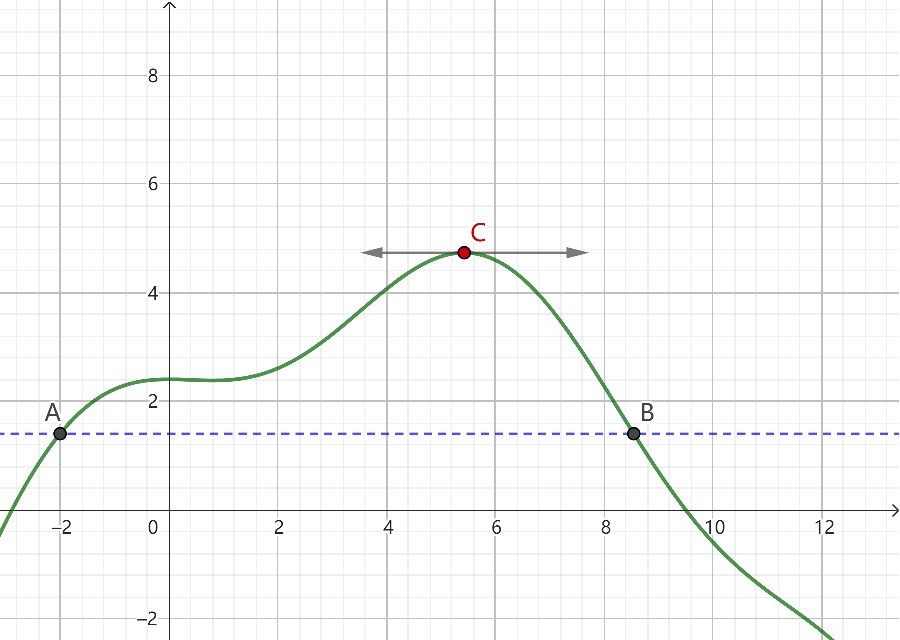
\includegraphics[width=0.6\textwidth]{tu/微变零值定理1.png}    
    \caption*{\texttt{函数满足}$f(a) = f(b)$\texttt{,于是会在某处附近变得水平。}}
\end{figure}

那么,函数曲线怎样的情况下会变得水平呢?一种情况就是“掉头”,即函数从左到右逼近这一点时,
函数值不断变大,但过了这一点,就不断变小了。或者反过来,从左到右逼近这一点时,不断变小,
但过了这一点,就不断变大了。

也就是说,函数在这一点附近达到局部的极大值或极小值时,会变得水平。

对于定理中提到的函数$f$,我们知道$f(a) = f(b)$。也就是说,把$a$看作起点,把$b$看作终点,
那么函数经历了一段变化后,函数值又回到了起始的水平。那么,直觉上,要么函数值一直不变,
要么总有“掉头”的一刻。
比如说,如果函数值一开始不断变大,那么,为了在终点变回原值,一定要在某一点“掉头”变小。
而该点就是微变为$0$的点。

要注意的是,这样的情形之所以存在,是因为函数满足“在闭区间$[a; b]$上连续,在开区间$(a; b)$上可微”的条件。
否则,我们想象中的“不断变大”、“掉头”都有可能因为函数“跳跃”、“突转”而不存在。

下面给出定理的证明:
\begin{proof}
    记$f(a) = f(b) = v$。如果$f$在$[a; b]$上恒等于$v$,那么任意挑选$(a; b)$中一点即可。

    否则,由于$f$在$[a; b]$上连续,根据闭区间极值定理,$f$在区间上有极大值$v_{\text{大}}$和极小值$v_{\text{小}}$。
    而这两个值不全等于$v$。不妨设极大值$v_{\text{大}}$不等于$v$。设$v_{\text{大}} = f(t)$,
    则$t\in(a; b)$。

    考虑$t$附近的变率:
    $$ \frac{f(x) - f(t)}{x - t}. $$
    由于$f$在$t$处有极大值,所以总有$f(x) \leqslant f(t)$。
    因此,$x<t$时,变率大于等于$0$;$x>t$时,变率小于等于$0$。
    $\partial f(t)$是$x$趋于$t$时,该变率的极限。
    根据极限传递不等关系的性质,变率在该点的左极限大于等于$0$,右极限小于等于$0$。
    而$f$在该点可微,因此左极限等于右极限,故都等于$0$。
    
    这就说明,$ \partial f(t) = 0$。
\end{proof}

我们研究的函数,不一定能满足$f(a) = f(b)$的条件。
不过,我们可以用一点技巧,把这个结论拓展到更一般的情况。

\begin{tm}{\textbf{微变中值定理}}\label{tm:2-4-10}
    如果函数$f$在闭区间$[a; b]$上连续,在开区间$(a; b)$上可微,
    那么,存在一点$t\in(a; b)$,使得
    $$ \partial f(t) = \frac{f(b) - f(a)}{b - a}.$$
\end{tm}

去掉了$f(a) = f(b)$的条件,相当于允许函数在该段区间有一个整体的变化趋势。
我们可以把这个整体的变化趋势用变率表示:$k = \frac{f(b) - f(a)}{b - a}$。
而中值定理告诉我们,区间中有一点,函数在其附近的变化趋势和整体趋势一样。

\begin{figure}[h]
    \centering
    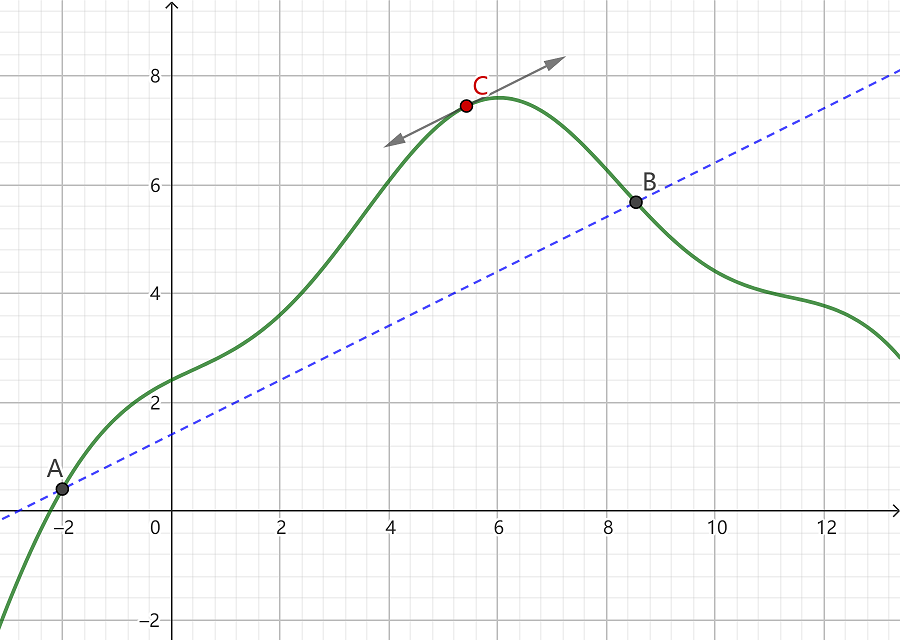
\includegraphics[width=0.6\textwidth]{tu/微变中值定理1.png}    
    \caption*{\texttt{可以把}$f(a) \neq f(b)$\texttt{视为考虑了整体变化的趋势。}}
\end{figure}

如果令$f(a) = f(b)$,那么$k=0$,这时我们得到微变零值定理。
如何把一般情况变为这种特殊情况呢?我们可以用过$f$在区间两端点的直线,大致描述函数的整体变化趋势:
$$ y = f(a) + k(x - a).$$
$x = a$时,$y = f(a)$,$x = b$时,$y = f(b)$。
那么,在函数中“剔除”这个趋势即可。

我们把函数“拆分”成两部分,一部分描述整体趋势,一部分描述函数在其中的“内部变化”。
$$ f(x) = {\color{magenta} f(a) + k(x - a)} + {\color{blue} g(x)}. $$
其中$g$的定义就是$g(x) = f(x) - f(a) - k(x - a)$。

那么,$f(a) + k(x - a)$就是$f$的趋势部分,$g$就是内部变化部分。$g(a) = g(b) = 0$。
$g$也在闭区间$[a; b]$上连续,在开区间$(a; b)$上可微。
对$g$运用微变零值定理可知,存在$t\in(a;b)$,使得$\partial g(t) = 0$。
然而,$\partial g = \partial f - k$。也就是说,$ \partial f(t) - k = 0$,即:
$$ \partial f(t) = k.$$
于是我们找到了满足要求的$t$,微变中值定理成立。

以上推理过程中,我们看到了函数变化和微变函数的关系。函数的单调性也能用微变描述。
\begin{tm}{\textbf{微变单调定理}}\label{tm:2-4-20}
    如果函数$f$在区间$I$上可微,那么$f$在$I$上单调递增(递减),
    当且仅当它在$I$上的微变总大于等于(小于等于)零。
\end{tm}

\begin{proof}
    如果$f$在$I$上单调递增,那么变率总大于等于$0$,因此微变作为变率的极限也总大于等于$0$。
    
    同理,$f$在$I$上单调递减,那么微变总小于等于$0$。

    反之,如果$f$在$I$上的微变总大于等于$0$,那么,对于$I$中任意两点$a < b$,根据微变中值定理,
    总有$c\in(a; b)$使得:
    $$f(b) - f(a) = \partial f(c) \cdot (b - a).$$
    而等式右边的项都大于等于$0$,所以$f(b) \geqslant f(a)$。这说明$f$在$I$上单调递增。
    
    同理,如果$f$在$I$上的微变总大于等于$0$,那么$f$在$I$上单调递减。
\end{proof}

\begin{sk}
    \mbox{} \\
    \indent 1. 微变零值定理中,如果去掉“在$(a; b)$上可微”,结论是否还成立?如果不成立,举一个反例。\\
    \indent 2. 微变单调定理中,如果要使得$f$在$I$上严格单调递增(递减),需要什么条件?\\
    \indent 3. 函数在一点微变率为$0$,是否说明该点是$f$在附近局部的极小值或极大值?
\end{sk}

\begin{xt}
    \mbox{} \\
    \indent 1. 证明:每个整式函数都是某个函数的微变函数。\\
    \indent 2. 已知函数$f$为:
    $$ f: \,\,\, x\mapsto \frac{\sin{x} + \cos{x}}{2 + \cos^2{x} - \sin{x}}.$$
    \indent 证明:对任意实数$a$,$f$在区间$(a; a + 2\pi)$上总有一处微变为$0$。\\
    \indent 3. 设函数$f$、$g$在区间$[a; b]$上连续,在$(a; b)$上可微。$g(a) \neq g(b)$,且$f$、$g$在任一点的微变率不同时为$0$。\\
    \indent 3.1. 设$k_f$为$f$从$a$到$b$的变率,$k_g$为$g$从$a$到$b$的变率,作函数:
    $$ h : \,\,\, x \mapsto k_g \cdot (f(x) - f(a)) - k_f \cdot (g(x) - g(a))$$
    \indent 证明:$h$在区间$[a; b]$上连续,在$(a; b)$上可微,且$h(a) = h(b) = 0$。\\
    \indent 3.2. 证明:存在$t\in(a; b)$,使得:
    $$ \frac{\partial f (t)}{\partial g (t)} = \frac{f(b) - f(a)}{g(b) - g(a)}.$$
    \indent 4.1. 证明:
    $$ \forall x > 0, \,\,\, \frac{1}{x+1} < \ln{(x+1)} - \ln{x} < \frac{1}{x}.$$
    \indent 4.2. 证明:函数$f: \,\,\,x \mapsto \left(1 + \frac{1}{x}\right)^x$在$(0;\infty)$上单调递增,
    函数$g: \,\,\,x \mapsto \left(1 + \frac{1}{x}\right)^{x+1}$在$(0;\infty)$上单调递减。(提示:考虑复合函数$\ln{f}$和$\ln{g}$。)\\
    \indent 4.3. 证明:$x$趋于正无穷时,函数$f$、$g$有极限,并给出这个极限的值。\\
    \indent 4.4. 设数列$\{v_n\}_{n\in\mathbb{N}}$的通项为:
    $$ \forall \,\, n\in\mathbb{N},\,\,\, v_n = \frac{1}{n+1} + \frac{1}{n+2} + \cdots + \frac{1}{2n}. $$
    证明:
    $$ \ln{(2n + 1)} - \ln{(n + 1)}  < v_n < \ln{(2n)} - \ln{(n)}. $$
    从而证明数列$\{v_n\}$收敛,并给出它的极限。\\
    \indent 5. 设有界函数$f$在实数集上可微,且它的微变函数$\partial f$在正无穷有极限$c$。证明:$c = 0$。(提示:使用反证法。)\\
    \indent 6. 设函数$f$在$a$处可微,且微变$\partial f(a) \neq 0$。\\
    \indent 6.1. 证明:存在$h>0$,使得对区间$(a-h;a+h)$中任意$x$,$f(x) = f(a)$当且仅当$x = a$。\\
    \indent 6.2. 如果函数$f$还在$a$附近可微,且微变函数$\partial f$在$a$处连续,证明:存在$h>0$,使得$f$在区间上是单射。

\end{xt}

\section{多次微变}
% 多次微变,k阶光滑
既然对可微的函数,可以定义它的微变函数,那么,如果微变函数仍然可微,我们就可以继续定义它的微变函数。
也就是说,只要条件允许,我们可以定义函数的多次微变函数。

举例来说,正弦函数$\sin$的微变函数是余弦函数$\cos$。而余弦函数$\cos$的微变函数是$-\sin$。
因此,我们可以说,正弦函数$\sin$的二次微变函数是$-\sin$。对于一点$a$,我们说正弦函数在$a$处
二次可微,二次微变率为$\sin{a}$。

一般来说,我们可以这样定义:
\begin{df}{\textbf{多次微变}}
    \mbox{} \\
    设函数$f$在区间$I$上可微。如果它的微变函数$\partial f$在$I$上仍然可微,就说$f$\textbf{二次可微}。
    $\partial f$在$I$上的微变函数称为$f$的\textbf{二次微变函数},简称\textbf{二次微变},记作$\partial^2 f$。
    
    依此类推,对正整数$k$,如果$f$的$k$次微变函数$\partial^k f$在$I$上仍然可微,就说$f$是$\boldsymbol{k+1}$\textbf{次可微}的。
    $\partial^k f$的微变函数称为$f$的$\boldsymbol{k+1}$\textbf{次微变函数},简称$\boldsymbol{k+1}$\textbf{次微变},记作$\partial^{k+1} f$。

    对于$I$中一点$a$来说,如果$f$是$k$次可微的,且$\partial^k f$在$a$处可微,
    就说$f$在$a$处$\boldsymbol{k+1}$\textbf{次可微},微变率称为$f$在$a$处的$\boldsymbol{k+1}$\textbf{次微变率}。

    如果对任意正整数$k$,$f$都是$k$次可微的,就说$k$\textbf{无穷可微}。
\end{df}

可以验证,前几节提及的显式函数,都是无穷可微的。
因为它们的微变总是由常见显式函数通过四则运算、复合、取反函数的方式组成。

比如,单项式函数$x\mapsto x^n$的$k$次微变为:
$$ \partial^k (x^n) = \left\{
    \begin{array}{ll}
        x\mapsto n(n-1)\cdots(n-k+1) x^{n-k} & \mbox{如果} k \leqslant n \\
        x\mapsto 0 & \mbox{如果} k > n
    \end{array}\right.
$$

指数函数$x\mapsto a^x$的$k$次微变为$x\mapsto (\ln{a})^k a^x$。
特别地,$x\mapsto e^x$的任意次微变都是自己。

正弦、余弦函数的多次微变和次数的奇偶性相关。
\begin{align*}
    \forall \,\,n\,\,\in\,\,\mathbb{Z}^+, \\
    \partial^{2n-1} \sin(x) &= (-1)^{n-1} \cos{x}, & \partial^{2n} \sin(x) &= (-1)^{n} \sin{x},  \\
    \partial^{2n-1} \cos(x) &= (-1)^{n} \sin{x}, & \partial^{2n} \cos(x) &= (-1)^{n} \cos{x},  
\end{align*}

两个$k$次可微函数$f$、$g$的和与差,仍然是$k$次可微函数,其$k$次微变函数为:
$$ \partial^k (f \pm g) = \partial^k f \pm \partial^k g $$
而它们的乘积也依然是$k$次可微函数,其$k$次微变函数为:
\begin{align*}
    \partial^k (f \cdot g) &= \partial^k f \cdot g + C_k^1 \partial^{k-1} f \cdot \partial g + \cdots + C_k^i \cdot \partial^{k-i} f \cdot  \partial^i g + \cdots + \cdot \partial^{k} g  \\
    &= \sum_{i=0}^k C_k^i \partial^{k-i} f \cdot  \partial^i g 
\end{align*}
这个表达式和二项式的展开一样,因为函数乘积的微变就是(一次的)二项式。

对于多次可微的函数,使用多次微变,可以给出类似微变中值定理的结论。
回顾微变中值定理,我们可以把它用来理解函数在一点附近的行为。对于符合条件的函数$f$,我们可以写出:
$$ f(a + h) = f(a) + \partial f(a + t) h.$$
其中$0<t<h$。我们把$f$在$a$附近的函数值$f(a+h)$表达为关于$h$的一次式,相比直接使用$a$处的微直观:
$$ f(a + h) \approx f(a) + \partial f(a) h,$$
使用$\partial f(a + t)$可以得到精确的关系,但这时$h$的系数是随着$h$变化的。
这与我们用平均速度来近似一样。我们希望$h$的系数只与$a$有关。
比如,如果可以把$f(a + h)$表示成:
$$ f(a + h) = f(a) + \partial f(a) h + w_2\partial^2 f(a + t) h^2,$$
其中$0<t<h$,$w_2$为常数系数。这样,我们就能具体地估计函数的微直观与精确值的误差。
当$h$很接近$0$的时候,$h^2$比$h$小得多,我们就可以忽略这一项。

一般来说,如果$f$多次可微,我们希望能有这样的近似表达式:
$$ f(a + h) = f(a) + \partial f(a) h + c_2 \partial^2 f(a) h^2 + \cdots + c_n \partial^n f(a) h^n + w_{n+1}\partial^{n+1} f(a + t) h^{n+1}.$$
即用关于$h$的多项式来近似表示$f(a + h)$的值。其中$c_2, \cdots c_n$是常数系数。
而$w_{n+1}\partial^{n+1} f(a + t) h^{n+1}$和$h$的$n+1$次方成正比,当$h$接近$0$时,就变成一个很小的误差项,
比前面次数更低的项小得多。这样,我们就可以通过关于$h$的多项式来估计$f(a + h)$的值。

\begin{tm}{\textbf{微变展开定理}}
    设$n$为正整数。已知函数$f$在包含实数$a$的区间$I$中$n+1$次可微,那么,对于$I$中另一个数$x$,
    存在介于$a$与$x$之间的数$c$,使得下式成立:
    \begin{align*}
        f(x) &= f(a) + \sum_{k=1}^n \frac{\partial^k f (a)}{k!}(x - a)^k + \frac{\partial^{n+1} f (c)}{(n+1)!}(x - a)^{n+1}.  \\
        &= P_n(x - a) + Y_n(x - a). 
    \end{align*}
    上式称为$f$在$a$处的$\boldsymbol{n}$\textbf{次微变展开}。
    其中$P_n$称为$f$在$a$处的$\boldsymbol{n}$\textbf{次微变展开多项式},
    $Y_n$称为$f$在$a$处展开的$\boldsymbol{n}$\textbf{次余项}。
    
\end{tm}

这个定理可以通过多次使用微变零值定理和中值定理得到(见附录$B$),可以看作微变中值定理的增强版本。
下面通过实际例子来看它的应用。

\begin{et}
    计算$\sin{\frac{\pi}{36}}$的值,精确到小数点后$5$位。
\end{et}

\begin{so}
    观察正弦函数的图像,它在$0$到$\frac{\pi}{2}$上单调递增。$\frac{\pi}{36}$相对于$\frac{\pi}{2}$很小。
    我们可以在$0$作多次微变展开,求$\sin{\frac{\pi}{36}}$的近似值。

    记$h = \frac{\pi}{36}$。由于正弦函数无穷可微,根据微变展开定理,把它在$0$处作$n$次展开,可得:
    $$ \sin{h} = \sin{0} + \sum_{k=1}^n \frac{\partial^k \sin (0)}{k!}h^k + Y_n. $$
    其中余项$Y_n$为:
    $$ Y_n = \frac{\partial^{n+1} \sin (c)}{(n+1)!}h^{n+1}. $$

    按题目要求,计算结果精确到小数点后$5$位。对此,我们希望使用前面的多项式来计算近似值,而余项$Y_n$就是近似误差。
    因此,我们要估计余项的大小。
    
    正弦函数的多次微变要么是余弦函数,要么是正弦函数,至多相差一个正负号,因此绝对值小于等于$1$。
    $h$的值大约在$0.08$到$0.1$之间,因此,$h^5$小于$10^{-5}$。考虑到余项中还有作为分母的$(n+1)!$,
    我们可以尝试令$n=3$。这时:
    \begin{align*}
        | Y_n| &= \left|\frac{\partial^{n+1} \sin (c)}{(n+1)!}h^{n+1}\right|  \\
        &= \frac{\left|\partial^{4} \sin (c)\right|}{4!}|h|^4  \\
        &\leqslant \frac{|h|^4}{4!}  \\
        &< \frac{10^{-4}}{24} < 5 \cdot 10^{-6}. 
    \end{align*}
    具体计算可知,$\frac{|h|^4}{4!} \approx 0.0000024$。
    因此误差足够小。

    % \sin(h) = 0.0871557427476581735580642708374735513777011561497026726137433675
    % h - h^3/6 = 0.0871557005802538165941859519079872293392595591884392781071638682
    % h = 0.0872664625997164788461845384244306356721435944270862728048595720

    接下来计算展开多项式$P_3(h)$的值。
    \begin{align*}
        P_3(h) &= \sin{0} + \frac{\cos (0)}{1!}h^1 - \frac{\sin (0)}{2!}h^2 - \frac{\cos (0)}{3!}h^3  \\
        &= h - \frac{h^3}{6}  \\
        &\approx 0.08716. 
    \end{align*}
    
    实际上,$\sin{\frac{\pi}{36}}$的值约为$0.08715574$,精确到小数点后$5$位为$0.08716$。
    因此近似计算结果是正确的。
\end{so}

一般来说,实践中,我们使用显式函数作为经验公式来描述、总结某些实验现象。
这时,如果显式函数多次可微,并且多次的微变大小可控(比如上面的正弦函数),
那么,通过合理估计余项的大小,我们可以把显式函数的值用整式近似,从而简化计算。

\begin{sk}
    \mbox{} \\
    \indent 1. 两函数的商的多次微变是否有规律?能否总结成统一的表达式?\\
    \indent 2. 两函数的复合函数的多次微变是否有规律?\\
    \indent 3. 函数可微次数是否越多越“好”?可微次数多代表什么?无穷可微的函数有什么“优点”?
\end{sk}

\begin{xt}
    \mbox{} \\
    \indent 1. 证明两函数乘积的多次微变公式。(提示:使用归纳法。)\\
    \indent 2. 求以下函数的多次微变函数。\\
    \indent 2.1. 求正切函数的$5$次微变函数。\\
    \indent 2.2. 求幂函数$x\mapsto x^r$的$k$次微变函数。\\
    \indent 2.3. 给定实数$a$,求函数$x\mapsto e^{ax}$的$k$次微变函数。\\
    \indent 2.4. 求函数$x \mapsto (ax^2 + bx + c)e^x$的$k$次微变函数。\\
    \indent 2.5. 求函数$x \mapsto x^2\ln{x}$的$k$次微变函数。\\
    \indent 3. 证明:对任意正整数$n$,函数$x\mapsto x^n e^{\frac{1}{x}}$的$n+1$次微变函数是
    $$x\mapsto \frac{(-1)^{n+1}}{x^{n+2}}e^{\frac{1}{x}}.$$
    \indent 4. $n$为正整数。$f$在区间$[a; b]$上$n$次可微。\\
    \indent 4.1. 证明:如果$f$在$[a; b]$中有$n+1$个不同的零点,那么有$c\in(a; b)$\\
    \indent 使得$\partial^n f(c) = 0$。\\
    \indent 4.2. 函数$f$在$[a; b]$上$n$次可微。证明:如果
    $$f(a) = \partial f(a) = \partial^2 f(a) = \cdots = \partial^{n-1} f(a) = f(b) = 0,$$
    \indent 那么有$c\in(a; b)$使得$\partial^n f(c) = 0$。\\
\end{xt}

\chapter{研究可微函数}

我们很早就学习了用平面上的曲线表示函数的方法来直观地理解函数。
函数的图像就是平面上的曲线。

不过,由于缺乏严谨描述实数和曲直质的语言,我们只用描点法来描述函数的图像。
画出函数图像上足够多的点,然后用线段将相邻的点连起来,并假设这样能近似表示函数的图像。

通过这样的近似图像,我们可以大致了解函数的性质,但无法严谨地讨论。

对于简单的函数,我们可以直接利用函数的表达式分析函数的性质。对于比较复杂的函数,
我们就需要更有力的工具。
学习了函数的微变之后,使用微变的知识,我们可以用严谨的方式,讨论曲线的直观性质。

\section{增减与极值}

我们学习过单调递增和单调递减函数的概念。函数的增减是我们希望了解的基本性质。

我们已经了解过一些基本的常见函数的增减性,比如正比例函数、反比例函数、幂函数、三角函数等。
对于较为复杂的函数,我们通过“增函数的复合仍然是增函数”、“增函数的反函数是增函数”等方法,可以推断一些函数的单调性。

微变是讨论函数局部变化的有力工具。使用微变的概念,我们可以讨论更一般的情况下,函数的增减变化。

对于可微的函数,我们有以下结论:
\begin{tm}{\textbf{微变率与函数增减的关系}}\label{tm:3-1-0}
    函数$f$在区间$I$上可微。
    \begin{itemize}
        \item 函数$f$在$I$上为常数函数,当且仅当$\partial f$在$I$上恒等于$0$。
        \item 函数$f$在$I$上单调递增(单调递减),当且仅当$\partial f$在$I$上总大于等于$0$(小于等于$0$)。
        \item 如果$\partial f$在$I$上总大于$0$(小于$0$),那么函数$f$在$I$上严格单调递增(严格单调递减)。
    \end{itemize} 
\end{tm}
以上结论可以使用微变率的定义和微变中值定理得到。可以看到,函数在一段区间内的增减变化,
与它在这段区间上的微变的正负性质是紧密相关的。
这是判定函数增减的有力工具。

\begin{et}
    研究函数$f:\,\,x\mapsto x + \frac{1}{x}$的增减性。
\end{et}

\begin{so}
    $f$在$\mathbb{R}^*$上有定义。易知$f$在定义域上可微。

    函数的增减性质与微变函数的正负性质相关。因此,求$f$的微变函数,得到:
    $$ \partial f(x) = 1 - \frac{1}{x^2} = \frac{x^2 - 1}{x^2}.$$
    分母$ x^2 $总大于$0$,因此$ \partial f $的正负性取决于二次函数$x^2 - 1$的正负性。
    
    根据二次函数的性质,$x^2 - 1$的正负性质为:
    $$ x^2 - 1 \left\{
        \begin{array}{cl}
            < 0 & \mbox{如果}x \in (-1; 1) \\
            = 0 & \mbox{如果}x = -1 \mbox{或} x = 1 \\
            > 0 & \mbox{如果}x \in (-\infty; -1)\cup (1; +\infty)\\
        \end{array}\right.
    $$
    因此,$f$在区间$(-\infty; -1]$上单调递增,在$x = -1$处达到极大值;
    然后在$[-1; 0)$上单调递减;$[-1; 0)$上单调递减;在$x = 1$处达到极小值;
    之后在$[1; +\infty)$上单调递增。

    可以看出,$f$在$-\infty$、$-1$、$0$、$1$、$+\infty$的情况,是我们了解$f$的几个“关键点”。
    容易算出在$-1$、$1$处,函数值分别为$f(-1) = -2$、$f(1) = 2$。
    
    $x$趋于负无穷时,$x$趋于负无穷,$\frac{1}{x}$趋于$0$,因此$f$趋于负无穷。

    $x$趋于正无穷时,$x$趋于正无穷,$\frac{1}{x}$趋于$0$,因此$f$趋于正无穷。

    $x$从左侧趋于$0$时,$\frac{1}{x}$趋于负无穷,因此$f$趋于负无穷。
    
    $x$从右侧趋于$0$时,$\frac{1}{x}$趋于正无穷,因此$f$趋于正无穷。

    综上,我们可以这样描述$f$的增减:随着$x$增大,$f$在区间$(-\infty; -1]$上从负无穷单调递增,
    在$x = -1$处达到极大值$f(-1) = -2$;
    然后在$[-1; 0)$上单调递减,在$x$趋于$0$时趋于负无穷。
    $f$在$(0; 1]$上从正无穷单调递减,在$x = 1$处达到极小值$f(1) = 2$;
    之后在$[1; +\infty)$上单调递增,趋于正无穷。
\end{so}

\begin{et}
    研究函数$f:\,\,x\mapsto x^2 e^{-2x}$的增减性。
\end{et}

\begin{so}
    $f$在$\mathbb{R}$上有定义。作为基本显式函数的复合函数,易知$f$在$\mathbb{R}$上可微。

    函数的增减性质与微变函数的正负性质相关。因此,求$f$的微变函数,得到:
    $$ \partial f(x) = (-2x^2 + 2x) e^{-2x}.$$
    指数函数$ e^{-2x} $总大于$0$,因此$ \partial f $的正负性取决于二次函数$-2x^2 + 2x$的正负性。
    
    根据二次函数的性质,$-2x^2 + 2x$的正负性质为:
    $$ -2x^2 + 2x \left\{
        \begin{array}{cl}
            > 0 & \mbox{如果}x \in (0; 1) \\
            = 0 & \mbox{如果}x = 0 \mbox{或} x = 1 \\
            < 0 & \mbox{如果}x \in (-\infty; 0)\cup (1; +\infty)\\
        \end{array}\right.
    $$
    因此,$f$在区间$(-\infty; 0]$上单调递减,在$x = 0$处达到极小值;
    然后在$(0; 1)$上单调递增,在$x = 1$处达到极大值;
    之后在$(1; +\infty)$上单调递减。

    可以看出,$f$在$-\infty$、$0$、$1$、$+\infty$的情况,是我们了解$f$的几个“关键点”。
    容易算出在$0$、$1$处,函数值分别为$f(0) = 0$、$f(1) = e^{-2} \approx 0.135$。
    
    $x$趋于负无穷时,$x^2$趋于正无穷,$e^{-2x}$趋于正无穷,因此$f$趋于正无穷。

    $x$趋于正无穷时,$x^2$趋于正无穷,$e^{2x}$趋于正无穷。需要研究两者的比值。
    $x > 1$时,$e^{2x} > 2^{2x}$,于是
    \begin{align*}
        f(x) &= \frac{x^2}{e^{2x}} < \frac{x^2}{2^x} \cdot \frac{1}{2^x}, 
    \end{align*} 
    而我们知道,对于正整数$n$,总有$2^n \geqslant n^2$。因此,
    $f(n) < 2^{-n}$,这说明$n$趋于无穷时,$f(n)$趋于$0$。
    而$f$在$(1;+\infty)$上单调递减且大于$0$,
    因此有极限。这个极限就是$f(n)$的极限,也就是$0$。

    综上,我们可以这样描述$f$的增减:随着$x$增大,$f$在区间$(-\infty; 0]$上从正无穷单调递减,在$x = 0$处达到极小值$f(0) = 0$;
    然后在$(0; 1)$上单调递增,在$x = 1$处达到极大值$f(1) = e^{-2} \approx 0.135$;
    之后在$(1; +\infty)$上单调递减,趋于$0$。
\end{so}

从例题可以知道,研究可微函数的增减可以分为几个固定步骤:
\begin{enumerate}
    \item 确定函数的定义域。
    \item 确定函数可微,求出函数的微变函数。
    \item 求处微变函数的零点,确定微变函数的正负性质。微变函数零点之中,使得正负号改变的点,就是函数的极值点。
    \item 根据微变函数的正负性质,确定函数的增减。
    \item 研究函数在正负无穷的极限、极值点处的值。
    \item 根据以上信息,描述函数的增减。
\end{enumerate}

\begin{et}
    研究函数$f:\,\,x\mapsto \ln(1 + \sin^2{x})$的增减性。
\end{et}

\begin{so}
    对任意实数$x$,$1 + \sin^2{x} > 0$,所以$f$在$\mathbb{R}$上有定义。

    作为基本显式函数的复合函数,易知$f$在$\mathbb{R}$上可微。

    函数的增减性质与微变函数的正负性质相关。因此,求$f$的微变函数,得到:
    $$ \partial f(x) = \frac{2\sin{x}\cos{x}}{1 + \sin^2{x}} = \frac{\sin{2x}}{1 + \sin^2{x}}.$$
    从$ \partial f $的表达式可知,分母总大于$0$。
    因此$ \partial f $的正负性就是分子,也就是$\sin{2x}$的正负性。

    根据正弦函数的性质,$\sin{2x}$是以$\pi$为周期的周期函数,它的正负性如下:
    $$ \sin{2x} \left\{
        \begin{array}{cl}
            > 0 & \mbox{如果}x \in (k\pi; k\pi + \frac{\pi}{2}),\,\,\, k\in\mathbb{Z} \\
            = 0 & \mbox{如果}x = \frac{k\pi}{2}, \,\,\,k\in\mathbb{Z} \\
            < 0 & \mbox{如果}x \in (k\pi - \frac{\pi}{2}; k\pi), \,\,\,k\in\mathbb{Z} \\
        \end{array}\right.
    $$
    因此,$f$的增减性质也是周期性的,以$\pi$为周期。以一个周期$[0, \pi]$为例。
    随着$x$增大,$f$在$[0, \frac{\pi}{2}]$上单调递增,在$\frac{\pi}{2}$处达到极大值,然后在$[\frac{\pi}{2}, \pi]$上单调递减。
    在$\pi$处达到极小值。
    
\end{so}

\begin{sk}
    \mbox{} \\
    \indent 1. 知道了函数的增减性质,能否画出函数图像?你认为还有哪些性质,能帮我们把函数的图像画得更好一点?\\
    \indent 2. 微变函数等于$0$的点,是否一定是极值点?如果不是的话,它有什么性质?    
\end{sk}

\begin{xt}
    \mbox{} \\
    \indent 1. 证明定理\ref{tm:3-1-0}。\\
    \indent 2. 研究以下函数的增减性质。\\
    \indent 2.1. $x\mapsto x^3 - x^5$。\\
    \indent 2.2. $x\mapsto \tan{\left(x - \frac{\pi}{6}\right)}$。\\
    \indent 2.2. $x\mapsto (1 - x^2) e^x$。\\
    \indent 2.3. $x\mapsto \frac{x^2 - 2}{(x + 1)(x - 3)}$。\\
    \indent 2.4. $x\mapsto e^{-\frac{1}{x}}$。\\
    \indent 2.5. $x\mapsto e^{-3x} \sin{(2x)}$。\\
    \indent 3. 设$I$为实数区间,$X$是$I$的子集。
    如果对$I$中任意$a < b$,都有$x\in I$使得$a<x<b$,就说$X$在$I$中\textbf{稠密}。
    设$f$在$I$上可微,微变函数$\partial f$在$I$上总大于等于$0$。
    记$A^+$为$I$中微变函数$\partial f$大于$0$的点的集合。\\
    \indent 3.1. 证明:如果$A^+$在$I$中稠密,那么$f$在$I$上严格单调递增。\\
    \indent 3.2. 证明:如果$f$在$I$上严格单调递增,那么$A^+$在$I$中稠密。
    
\end{xt}


 \section{局部性质}
 % 高阶无穷小

研究函数的增减性质时,我们发现,需要关注函数在一些“关键点”的行为。
如果函数在“关键点”有定义,那么我们只需要取函数值即可。
如果“关键点”是正负无穷,或者函数在“关键点”没有定义,那么我们需要特别研究函数在这些地方附近的行为。
我们把这样的性质称为函数的局部性质。

为此,我们再次说明“附近”的严格定义:\textbf{一点“附近”指它的某个邻域}。
而邻域的概念我们已经学习过了,这里再严谨地定义一次:
\begin{df}{\textbf{邻域}}
    对于实数$a$,我们把包含$a$的开区间$I$称为$a$的\textbf{邻域}。为了方便,我们一般取对称的开区间$(a-h; a+h)$,
    其中$h>0$是足够小的实数,以免涉及到别的区域。这样邻域记为$I_h(a)$。

    如果涉及函数$f$,那么在提及$a$的邻域时,一般考虑以上区间和$f$定义域的交集。
    但记法不变,仍然是$I_h(a)$。读者需要理解,这里指的是关于$f$有定义的部分。

    比如,如果$f$在$a$附近有定义,但在$a$处无定义,
    那么交集就是在$a$的邻域中去掉$a$得到的子集,称为$a$的\textbf{去心邻域}。

    显然,去心邻域就是$a$左右的两个开区间。
    比如,$(a-h; a+h)$对应的去心邻域就是$(a-h; a)\cup(a; a+h)$。
    这种情况可以记为$\overset{\circ}{I}_h(a)$。

    如果我们只希望讨论$a$的一侧,那么可以只取$a$的邻域小于等于$a$或大于等于$a$的部分,
    称为$a$的\textbf{左邻域}、\textbf{右邻域}。

    对于正负无穷,我们把形如$[H; +\infty)$、$(H; +\infty)$或$(-\infty; H]$、$(-\infty; H)$的
    区间称为它们的邻域,记为$I_H(+\infty)$、$I_H(-\infty)$。
\end{df}

研究函数的局部行为,也就是研究函数在特定点或者无穷远点附近的行为。

\begin{ex}
    \indent 1. 比较函数$f_1: x\mapsto x$和$f_2: x\mapsto x^2$在$0$附近的行为。\\
    \indent 2. 比较函数$f_1: x\mapsto \frac{1}{x}$和$f_2: x\mapsto \frac{1}{x^2}$在$0$附近的行为。
\end{ex}

对于第一个例子中的两个函数,我们知道,两者在$x$沿右侧趋于$0$时都趋于$0$。但$f_2$比$f_1$要快得多。比如,令$x=0.01$,
则$f_1(x) = 0.01$,而$f_2(x) = 0.0001$;令$x=0.001$,则$f_1(x) = 0.001$,而$f_2(x) = 0.0000\dlim{01}$。

对于第二个例子中的两个函数,我们知道,两者在$x$沿右侧趋于$0$时都趋于正无穷。但$f_2$比$f_1$要快得多。比如,令$x=0.01$,
则$f_1(x) = 100$,而$f_2(x) = 1\dlim{0000}$;令$x=0.001$,则$f_1(x) = 1000$,而$f_2(x) = 100\dlim{0000}$。

为了比较不同函数的局部行为,我们需要把“趋于无穷”、“趋于零”更细分。

\begin{df}{\textbf{无穷的阶}}
    设$f$、$g$是从区间$I$到$\mathbb{R}$的函数,$a\in I$\footnote{注意:这里的$a$也包括正负无穷。}。

    \indent 1. 如果对任意$r>0$,都有$a$的邻域$I_a(h)$,使得
    $$ \forall x \in I_a(h), \,\,\, |f(x)| \leqslant r |g(x)|,$$
    \indent 就说相比于$g$,$f$在$a$附近\textbf{可以忽略}。记为:
    $$ f \oveq{a} \olim{g}$$
    \indent 如果$x$趋于$a$时,$f$、$g$都趋于无穷,就说$g$是$f$的\textbf{高阶无穷大}。\\
    \indent 如果$x$趋于$a$时,$f$、$g$都趋于零,就说$f$是$g$的\textbf{高阶无穷小}。

    \indent 2. 如果有$a$的邻域$I_a(h)$和$M > 0$,使得
    $$ \forall x \in I_a(h), \,\,\, |f(x)| \leqslant M |g(x)|,$$
    \indent 就说$f$在$a$附近\textbf{受制于}$g$。记为:
    $$ f \oveq{a} \Olim{g}$$
    \indent 3. 如果$f$在$a$附近受制于$g$,而$g$也受制于$f$,就说两者等阶。\\
    \indent $f$是$g$的\textbf{同阶无穷大}或\textbf{同阶无穷小}。记为:
    $$ f \oveq{a} \Tlim{g}$$

    \indent 4. 如果$f - g$相比$g$可以忽略,就说$f$和$g$在$a$附近\textbf{等价},\\
    \indent $f$是$g$的\textbf{等价无穷大}或\textbf{等价无穷小}。
    $$ f \eqlim{a} g$$

\end{df}

简单来说,越高阶的无穷大(无穷小),表示趋于无穷(零)的速度不是一个级别的。
同阶的无穷,趋于无穷(零)的速度虽然有快慢,但仍然在同一个级别。
等价的无穷,趋于无穷(零)的速度相同。

在前面第一个例子中,$f_1: x\mapsto x$和$f_2: x\mapsto x^2$在$0$附近都是无穷小,但
对任意$r > 0$,我们都可以设$h = r$,这样,只要$|x| < r$,就有$|x^2| < r|x|$。
这说明$f_2$是$f_1$的高阶无穷小。

同理,第二个例子中,$f_1: x\mapsto \frac{1}{x}$和$f_2: x\mapsto \frac{1}{x^2}$在$0$附近都是无穷大。
但对任意$r > 0$我们都可以设$h = r$,这样,只要$|x| < r$,就有$|\frac{1}{x}| < r|\frac{1}{x^2}|$。
这说明$f_2$是$f_1$的高阶无穷大。

从定义来看,无穷的阶和极限很相似。两个函数在局部的无穷关系,也可以用两者比值的极限来表示:
\begin{itemize}
    \item $f$在$a$附近相比$g$可以忽略,当且仅当$\lian{x\to a} \frac{f}{g} = 0.$
    \item $f$在$a$附近与$g$等价,当且仅当$\lian{x\to a} \frac{f}{g} = 1.$
    \item 如果$\lian{x\to a} \frac{f}{g} > 0$,那么$f$在$a$附近是$g$的同阶无穷大。
\end{itemize}

我们可以把已知的说法转换成无穷的阶的“语言”。
比如,函数$f \oveq{a} \olim{1}$,表示$f$在$a$处趋于$0$。
又如,函数$f \oveq{a} \Olim{1}$,表示$f$在$a$附近有界。

根据无穷的阶的定义,我们还可以“开发”出一些“运算法则”。当然,它们只是用无穷的阶的“语言”,
把按照极限定义得到的直接推论复述一遍。
\begin{enumerate}
    \item 如果$f_1 \oveq{a} \olim{g_1}$,$f_2 \oveq{a} \olim{g_2}$,那么$f_1 f_2 \oveq{a} \olim{g_1 g_2}$。
    \item 如果$f_1 \oveq{a} \Olim{g_1}$,$f_2 \oveq{a} \Olim{g_2}$,那么$f_1 f_2 \oveq{a} \Olim{g_1 g_2}$。
    \item 如果$f \oveq{a} \Olim{g}$,那么对任意正整数$n$,$f^n \Olim{a}{g^n}$。
\end{enumerate}

我们可以用无穷的阶来更细致地刻画函数的局部性质。比如,在上一章中,我们研究了正弦函数在$0$附近的近似表示。
在$0$附近使用微变展开定理,正弦函数可以写成:
$$ \sin{h} = \sin{0} + \sum_{k=1}^n \frac{\partial^k \sin (0)}{k!}h^k + Y_n. $$
其中余项$Y_n$为:
$$ Y_n = \frac{\partial^{n+1} \sin (c)}{(n+1)!}h^{n+1}. $$
这说明正弦函数可以表示成多项式函数$P_n :h \mapsto \sin{0} + \sum_{k=1}^n \frac{\partial^k \sin (0)}{k!}h^k$与余项函数$h\mapsto Y_n(h)$
的和。而我们已经证明了这个余项函数受制于$h\mapsto h^{n+1}$,因此是$P_n$任一项的高阶无穷小。
因此,正弦函数在$0$附近可以用$P_n$来近似表示。

把函数用多项式近似表示,有什么好处呢?
把不同的函数统一用多项式近似表示,我们就能够(在局部)比较各种不同的函数了。

比如,我们知道$\sin{x}$和$\ln{(1+x)}$在$0$附近都约等于$0$。
那么比值$\frac{\sin{x}}{\ln{(1 + x)}}$在$0$附近是什么样子的呢?

首先利用微变展开定理把两者用多项式和余项表示。
\begin{align*}
    \sin{x} &= \sin{0} + \sum_{k=1}^n \frac{\partial^k \sin (0)}{k!}x^k + \mathit{o}(x^n).  \\
    \ln{(1 + x)} &= \ln{1} + \sum_{k=1}^n \frac{\partial^k \ln (1)}{k!}x^k + \mathit{o}(x^n).  
\end{align*}
然后从最“低阶”的无穷小开始对比。
\begin{align*}
    \sin{x} &= x - \frac{x^3}{6} + \frac{x^5}{120} + \cdots + \mathit{o}(x^n).  \\
    \ln{(1 + x)} &= x - \frac{x^2}{2} + \frac{x^3}{3} + \cdots + \mathit{o}(x^n). 
\end{align*}
$\sin{x}$和$\ln{(1+x)}$的“最大项”都是$x$,之后$\ln{(1+x)}$是$- \frac{x^2}{2}$,而$\sin{x}$是$- \frac{x^3}{6}$。
因此,我们可以写出它们的比值:
\begin{align*}
    \frac{\sin{x}}{\ln{(1 + x)}} &= \frac{x - \frac{x^3}{6} + \olim{x^3}}{x - \frac{x^2}{2} + \olim{x^2}}  \\
    &= \frac{1 - \olim{x}}{1 - \frac{x}{2} + \olim{x}}  \\
    &= \frac{(1 - \olim{x})\left(1 + \frac{x}{2} + \olim{x}\right)}{\left(1 - \frac{x}{2} + \olim{x}\right)\left(1 + \frac{x}{2} + \olim{x}\right)}  \\
    &= \frac{1 + \frac{x}{2} + \olim{x}}{1 + \olim{x}}  \\
    &= \left(1 + \frac{x}{2} + \olim{x}\right)(1 + \olim{x})  \\
    &= 1 + \frac{x}{2} + \olim{x} 
\end{align*}
也就是说,在$0$附近,$\sin{x}$和$\ln{(1+x)}$的比值大约是$1 + \frac{x}{2}$,余项是关于$x$的高阶无穷小。

把函数在$0$附近用一次整式和高阶无穷小表示,我们把这样的结果称为函数在$0$附近的一次展开。

我们把上面的方法称为\textbf{局部展开法}。简单来说,如果能够把函数在局部表示成多项式与高阶无穷小的和,
那么,通过无穷的阶的运算,我们可以细致地分析函数的局部性质。从一些常见函数的局部展开(见附录$B$)出发,
我们可以比较准确地刻画较为复杂的函数的局部性质。

\begin{et}
    求极限:
    $$ \lian{x\to +\infty} \frac{\left(1 + \frac{1}{x}\right)^{x^2}}{e^x}.$$
\end{et}

\begin{so}
    要求极限的函数由分子分母两部分组成。分子看起来很像$\left(1 + \frac{1}{x}\right)^{x}$,
    也就是$x$趋于正无穷时极限为$e$。不过指数从$x$换成了$x^2$。

    既然分子分母都和指数函数有关,我们可以把整个函数取对数,得到:
    $$ \ln{\frac{\left(1 + \frac{1}{x}\right)^{x^2}}{e^x}} = x^2 \ln{\left(1 + \frac{1}{x}\right)} - x.$$
    显然,等式右边比较难估计的是对数函数的部分。
    $x$趋于正无穷时,$\frac{1}{x}$趋于$0$。我们把$\ln{\left(1 + \frac{1}{x}\right)}$展开,得到:
    $$ \ln{\left(1 + \frac{1}{x}\right)} \oveq{+\infty} \frac{1}{x} - \frac{1}{2x^2} + \olim{\frac{1}{x^2}}$$
    因此,
    \begin{align*}
        x^2 \ln{\left(1 + \frac{1}{x}\right)} - x &\oveq{+\infty} x^2 \left(\frac{1}{x} - \frac{1}{2x^2} + \olim{\frac{1}{x^2}}\right) - x  \\
        &\oveq{+\infty} x -\frac{1}{2} + \olim{1} - x  \\
        &\oveq{+\infty} -\frac{1}{2} + \olim{1} 
    \end{align*}
    也就是说,
    $$ \lian{x\to +\infty} x^2 \ln{\left(1 + \frac{1}{x}\right)} - x = -\frac{1}{2}. $$
    于是
    $$ \lian{x\to +\infty} \frac{\left(1 + \frac{1}{x}\right)^{x^2}}{e^x} = e^{\lian{x\to +\infty}  x^2 \ln{\left(1 + \frac{1}{x}\right)} - x} = \frac{1}{\sqrt{e}}. $$
\end{so}

最后的问题:具有怎样性质的函数,才能在局部表示成多项式与高阶无穷小的和呢?我们有以下定理(证明见附录$B$):
\begin{tm}{\textbf{局部展开定理}}
    设$n$为正整数。函数$f$在区间$I$上$n$次可微,且$n$次微变函数在$I$上连续。那么,对于$a\in I$,
    $f$可以写成以下形式:
    $$ \forall x \in I , \quad f(x) = f(a) + \sum_{k=1}^n \frac{\partial^k f (a)}{k!}(x - a)^k + (x - a)^n h(x). $$
    其中$h$是一个在$I$上连续,在$a$处趋于$0$的函数。
\end{tm}

\begin{sk}
    \mbox{} \\
    \indent 1. 说明:等价无穷大(无穷小)是一种等价关系。\\
    \indent 2. 你认为,我们已知的关系中,什么关系和函数“可忽略”、“受制于”的关系最像?给出你的理由。\\
    \indent 3. 函数在局部是否一定可以用多项式近似表示?如果是,说明理由。如果不是,给出反例。\\\
    \indent 4. 如果$f_1 \eqlim{a} g_1$,$f_2\eqlim{a} g_2$,是否有$f_1 + f_2\eqlim{a} g_1 + g_2$?
\end{sk}

\begin{xt}
    \mbox{} \\
    \indent 1. 证明:\\
    \indent 1.1. 如果$f \eqlim{a} g$,$g \oveq{a} \olim{h}$,那么$f \oveq{a} \olim{h}$。\\
    \indent 1.2. 如果$f \eqlim{a} g$,$g \oveq{a} \Olim{h}$,那么$f \oveq{a} \Olim{h}$。\\
    \indent 1.3. 如果$f \oveq{a} \olim{g}$,$g \oveq{a} \Olim{h}$,那么$f \oveq{a} \olim{h}$。\\
    \indent 1.4. 如果$f \eqlim{a} \olim{g}$,$g \oveq{a} \Olim{h}$,那么$f \oveq{a} \olim{h}$。\\
    \indent 2. 设$a, b$为正数。证明:\\
    \indent 2.1. $x^a \oveq{+\infty} \olim{e^{bx}}$。\\
    \indent 2.2. $e^{-bx} \oveq{+\infty} \olim{|x|^{-a}}$。\\
    \indent 2.3. $\ln^{a}{x} \oveq{+\infty} \olim{x^{b}}$。\\
    \indent 2.4. $|\ln{x}|^{a} \oveq{0} \olim{|x|^{-b}}$。\\
    \indent 3. 证明:\\
    \indent 3.1. 在$0$附近,$\frac{1}{1 - x^2} = 1 + x^2 + \olim{x^2}$。\\
    \indent 3.2. 在$0$附近,$x^2 \cdot \olim{x^3} = \olim{x^5}$。\\
    \indent 3.3. 在$0$附近,$e^x - \sqrt{1 + x} = \frac{x}{2} + \frac{5x^2}{8} + \frac{7x^3}{48} + \olim{x^3}$。\\
    \indent 3.4. 在$0$附近,偶函数的局部展开只有偶数次项,奇函数的展开只有奇数次项。\\
    \indent 4. 在局部展开以下函数:\\
    \indent 4.1. 在$0$附近将$x\mapsto \frac{\sqrt{1 + x}}{1 - x^2}$作三次展开。\\
    \indent 4.2. 在$0$附近将$x\mapsto \frac{\cos{x} - 1}{\ln^2{(1 + x)}}$作三次展开。\\
    \indent 4.3. 在$0$附近将$x\mapsto \tan{(x)} - \frac{x}{1 + x}$作四次展开。\\
    \indent 4.4. 在$0$附近将$x\mapsto (1 - \ln{(1 + x)})e^{-x}$作四次展开。\\
    \indent 4.5. 在$2$附近将$x\mapsto x^2\ln{(x - 1)}$作三次展开。\\
    \indent 4.6. 在$1$附近将$x\mapsto (1 - x)\ln{(x^2 - 1)}$作三次展开。\\
    \indent 5. 使用局部展开法研究以下的极限:\\
    $$
    \begin{array}{ll}
        1. \quad \lian{x\to 0} \frac{\cos{x} - 1}{x^2} & \qquad 2. \quad \lian{x\to 0} \frac{1}{x \left(e^x - 1\right)} - \frac{1}{x^2} \\
        3. \quad \lian{x\to +\infty} \frac{1}{x}\ln{\left(\frac{e^x - 1}{x}\right)} & \qquad 4. \quad \lian{x\to 0} \frac{2x}{\ln{(1+x)} - \ln{(1-x)}} 
    \end{array}
    $$
    \indent 6. 如果$x \mapsto \frac{e^{x} + e^{ax} - 2}{x^2}$在$0$处有极限,求实数$a$可能的取值,并计算相应的极限。
\end{xt}

\section{凹凸性质}

要了解函数的性质,仅靠增减性质是不够的。举例来说,
$x\mapsto \sqrt{x}$和$x\mapsto x^2$在$[0;1]$上都是增函数,从$0$增长到$1$。
但两者的图像有很大差异。前者的图像是向上凸出的曲线,后者则向下凸出。

我们把函数形状分为两类,形如$x\mapsto \sqrt{x}$的称为\textbf{上凸},
把形如$x\mapsto x^2$的称为\textbf{下凸}。更严谨的定义如下:

\begin{df}{\textbf{函数的凸性}}
    \mbox{} \\
    函数$f$区间$I$上有定义。
    \begin{itemize}
        \item 如果对$I$中任意两点$x$、$y$,以及任意$0 \leqslant c \leqslant 1$,都有
        $$ f(cx + (1 - c)y) \leqslant cf(x) + (1 - c)f(y), $$
        就说$f$在区间$I$\textbf{下凸}。
        \item 如果对$I$中任意两点$x$、$y$,以及任意$0 < c < 1$,都有
        $$ f(cx + (1 - c)y) < cf(x) + (1 - c)f(y), $$
        就说$f$在区间$I$\textbf{严格下凸}。
        \item 如果对$I$中任意两点$x$、$y$,以及任意$0 \leqslant c \leqslant 1$,都有
        $$ f(cx + (1 - c)y) \geqslant cf(x) + (1 - c)f(y), $$
        就说$f$在区间$I$\textbf{上凸}。
        \item 如果对$I$中任意两点$x$、$y$,以及任意$0 < c < 1$,都有
        $$ f(cx + (1 - c)y) > cf(x) + (1 - c)f(y), $$
        就说$f$在区间$I$\textbf{严格上凸}。
    \end{itemize}
\end{df}

不难验证,前面提及的$x\mapsto x^2$和$x\mapsto \sqrt{x}$和$x\mapsto x^2$分别在$[0;1]$严格上凸、严格下凸。

\begin{figure}[h]
    \centering
    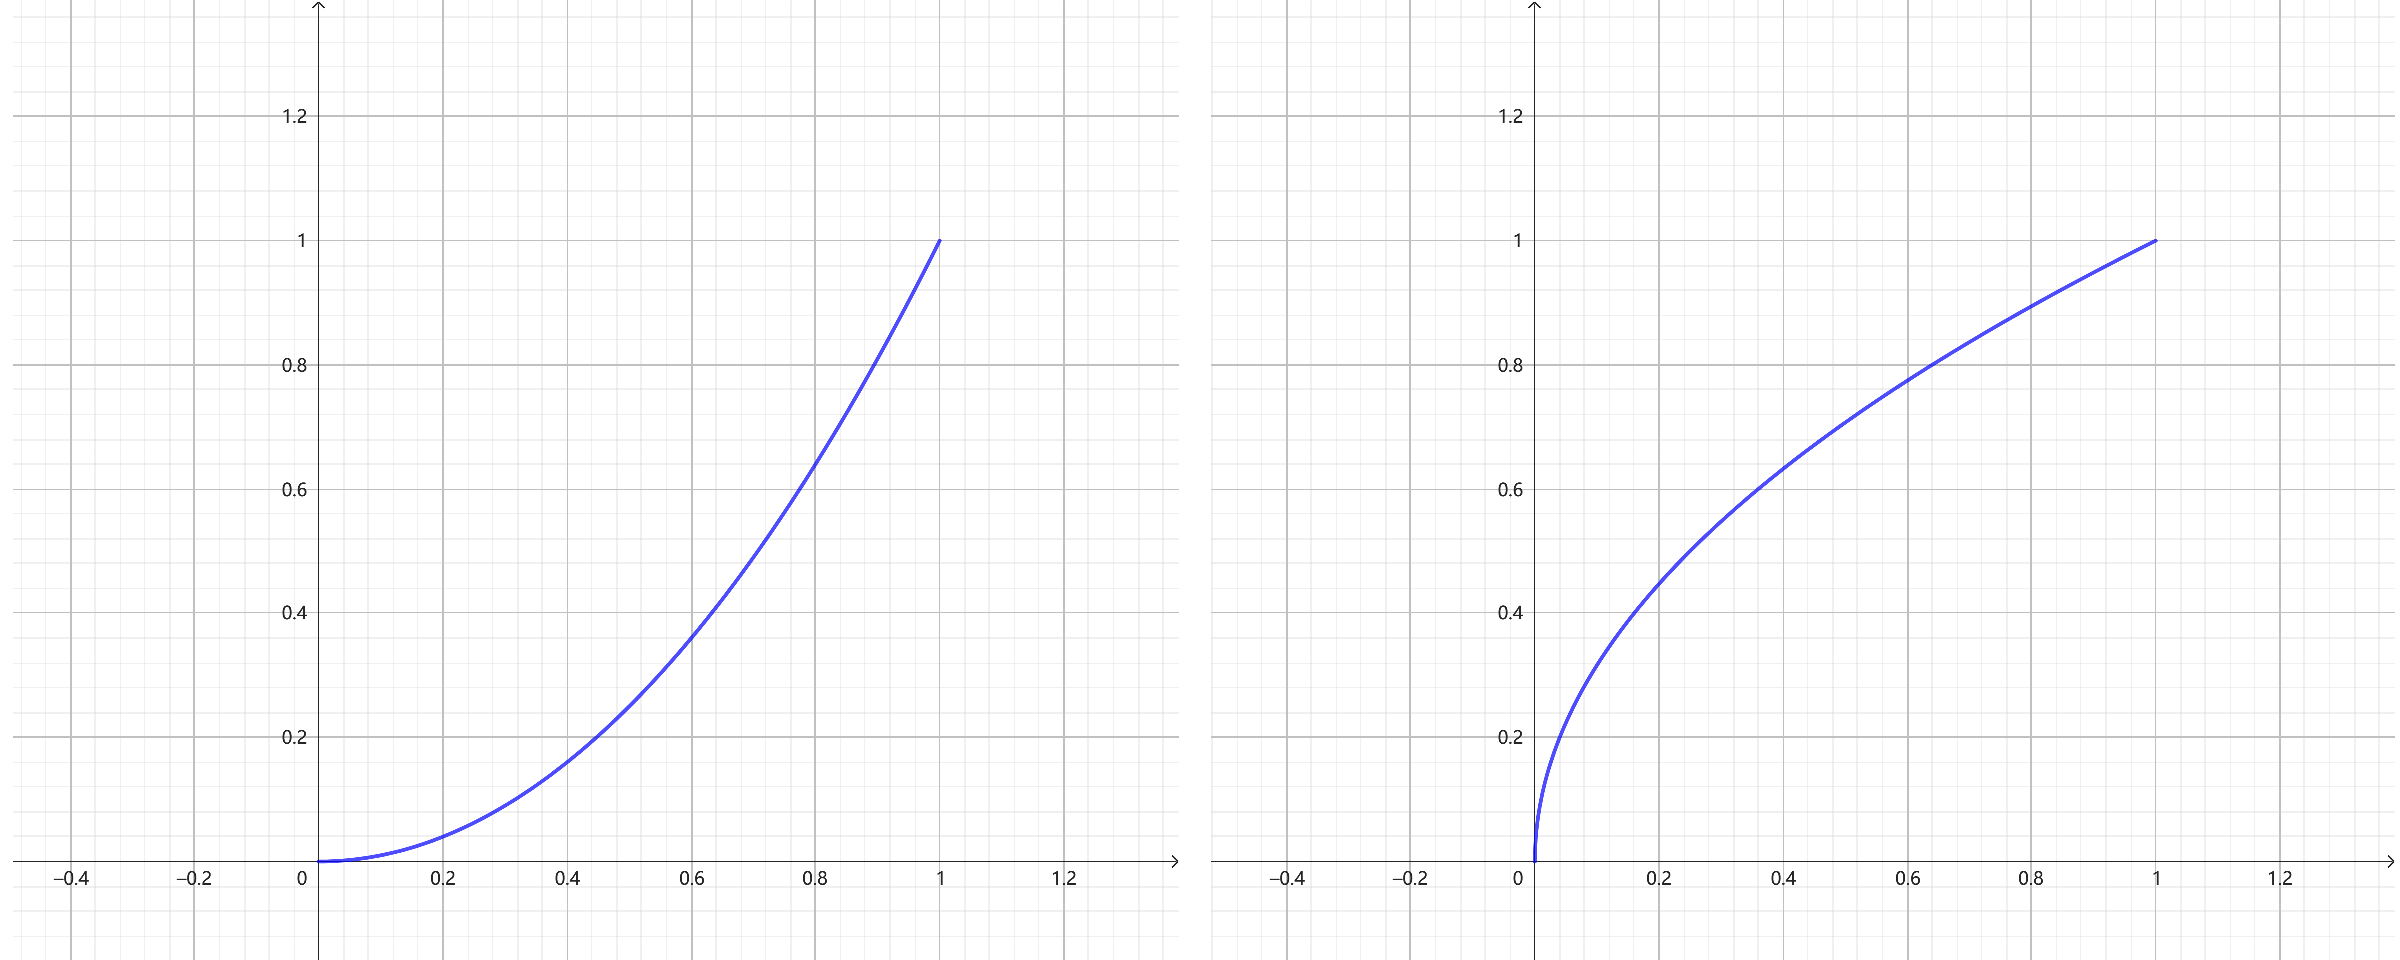
\includegraphics[width=0.8\textwidth]{tu/凹凸函数1.png}
    \caption*{$x\mapsto x^2$\texttt{(左)严格下凸,}$x\mapsto \sqrt{x}$\texttt{(右)严格上凸。}}
\end{figure}

设$z = cx + (1 - c)y$,可得$c = \frac{y - z}{y - x}$。带入凸性的定义,就可以得到用变率描述的版本。
比如,下凸的定义变为:对$I$中任意三点$x < z < y$,都有
$$ \frac{f(z) - f(x)}{z - x} \leqslant \frac{f(z) - f(y)}{y - z}. $$
或者说,从$x$到$z$的变率,小于等于从$z$到$y$的变率。换句话说,\textbf{函数下凸,就是变率不断变大}。
反之,\textbf{函数上凸,就是变率不断变小}。

\begin{figure}[h]
    \centering
    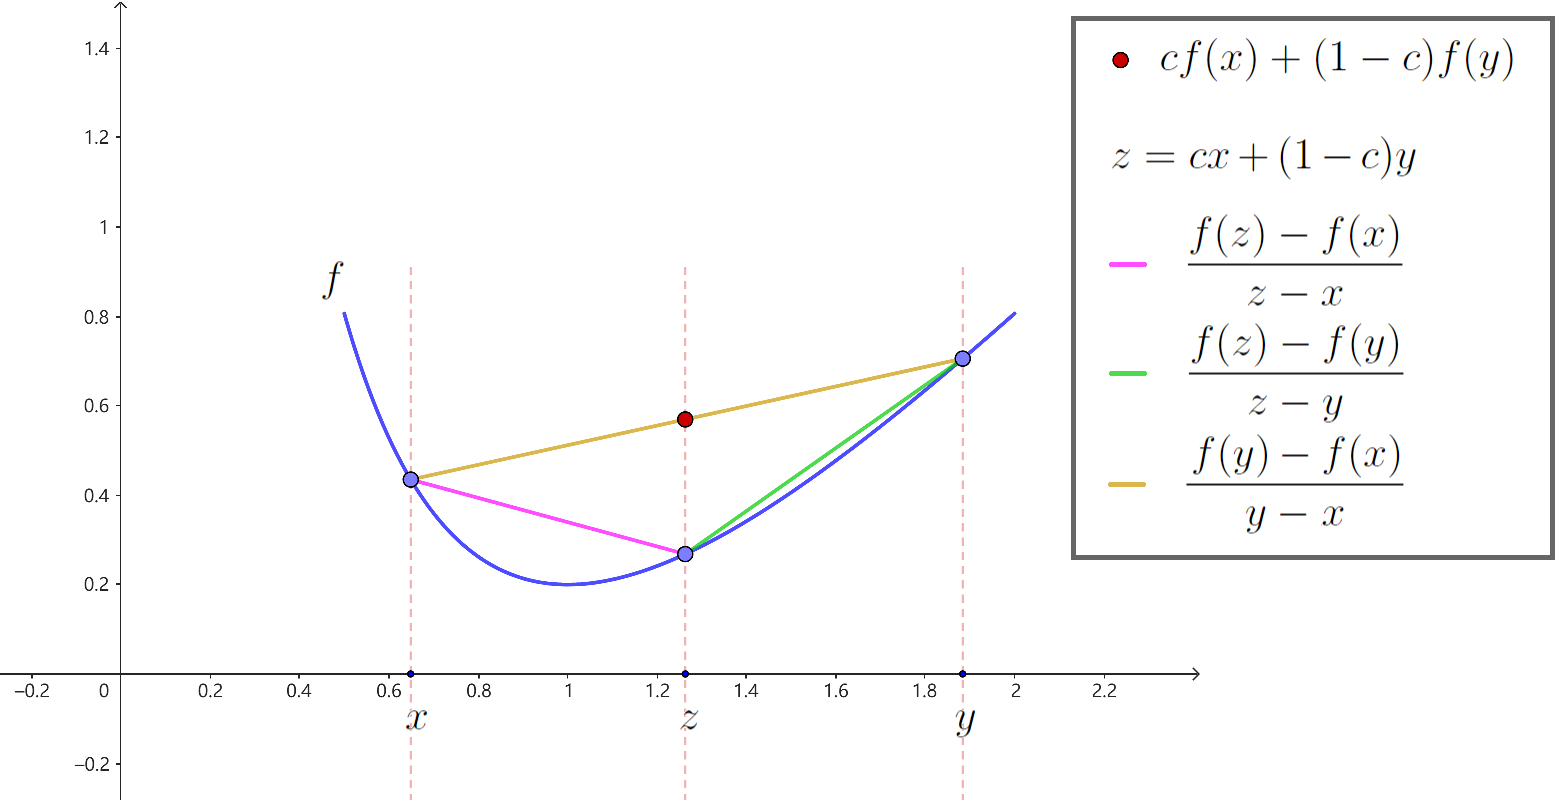
\includegraphics[width=0.8\textwidth]{tu/凸函数变率1.png}
\end{figure}

直观来看,设函数在$[a; b]$上有定义。
考虑以函数在两端的点$(a,\,\, f(a))$、$(b,\,\, f(b))$连成的线段。
如果函数下凸,那么在$(a;b)$上,函数图像总在线段下方;
如果函数上凸,那么在$(a;b)$上,函数图像总在线段上方。

对于简单的函数,可以按定义确定函数的凸性。
比如,$x\mapsto x^n$在$n>1$时是下凸函数,$x\mapsto x^\frac{1}{n}$在$n>1$时是上凸函数。
但对于比较复杂的函数,直接按定义较难确定函数的凸性。为此,我们需要更方便的判定方法。
如果函数可微,从凸性和变率的关系,不难想到以下的判定方法(证明见附录$B$):

\begin{tm}{\textbf{凸性与微变}}
    设函数$f$在区间$I$上可微。
    \begin{itemize}
        \item $f$在$I$下凸,当且仅当$\partial f$在$I$上单调递增。
        \item $f$在$I$上凸,当且仅当$\partial f$在$I$上单调递减。
        \item $f$在$I$严格下凸,当且仅当$\partial f$在$I$上严格单调递增。
        \item $f$在$I$严格下凸,当且仅当$\partial f$在$I$上严格单调递减。
    \end{itemize}
\end{tm}

如果函数$f$二次可微,那么我们有更简便的判定方法:
\begin{tm}\textbf{凸性与二次微变}
    设函数$f$在区间$I$上二次可微。
    \begin{itemize}
        \item $f$在$I$下凸,当且仅当$\partial^2 f$在$I$上总大于等于$0$。
        \item $f$在$I$上凸,当且仅当$\partial^2 f$在$I$上总小于等于$0$。
    \end{itemize}
\end{tm}

\begin{proof}
    只需证明$\partial f$在$I$上单调递增当且仅当$\partial^2 f$在$I$上总大于等于$0$。
    对可微函数$\partial f$使用定理\ref{tm:3-1-0}即可。
\end{proof}

用这个方法,我们能够轻松判定大多数常见显式函数的凸性,因为它们都二次可微。

幂函数$x\mapsto x^a$当$a>1$时是下凸的,当$0<a<1$时是上凸的;$a<0$时,在$(0;+\infty)$上是下凸的。

指数函数总是下凸的,对数函数总是上凸的。

正弦函数在每个周期$[2k\pi, \,\, 2(k+1)\pi)$前半是上凸的,后半是下凸的。
正切函数也是如此,在每个周期$(k\pi-\frac{\pi}{2}, \,\, k\pi+\frac{\pi}{2})$前半是上凸的,后半是下凸的。

如果函数的二次微变在某点$a$变号,就说$a$是函数的\textbf{拐点}。
比如,$x\mapsto x^3$在$0$处有拐点。它的二次微变在$x<0$时小于$0$,在$x>0$时大于$0$。
随着$x$增大,函数在$0$处从上凸转为下凸。

在函数的增减性质分析基础上,加入凸性的分析,就大致完成了对函数性质的初步分析。
有了这些分析结果,我们就能大致画出函数的图像。

\begin{et}
    研究函数$f:\,\,x\mapsto x^2 e^{-2x}$。
\end{et}

\begin{so}

    之前我们已经研究了$f$的增减性质。随着$x$增大,$f$在区间$(-\infty; 0]$上从正无穷单调递减,在$x = 0$处达到极小值$f(0) = 0$;
    然后在$(0; 1)$上单调递增,在$x = 1$处达到极大值$f(1) = e^{-2} \approx 0.135$;
    之后在$(1; +\infty)$上单调递减,趋于$0$。

    在此基础上,我们加上对函数凸性的研究。

    $f$在$\mathbb{R}$上有定义。容易验证$f$在$\mathbb{R}$上二次可微。二次微变函数为:
    $$ \partial^2 f (x) = 2(2x^2 - 4x + 1)e^{-2x}.$$
    $e^{-2x}$总大于零,所以二次微变的零点为$2x^2 - 4x + 1$的根,即:
    $$  
        \left\{ 
            \begin{array}{cl}
                x_1 &= \frac{2 + \sqrt{2}}{2} \\
                x_2 &= \frac{2 - \sqrt{2}}{2} 
            \end{array}
        \right.
    $$
    根据二次函数的性质,$f$的二次微变在$(-\infty; x_1)$、$(x_2; +\infty)$上大于零,
    在$(x_1; x_2)$上小于零。因此,$x_1$、$x_2$是函数$f$的拐点。$f$在$(-\infty; x_1)$、$(x_2; +\infty)$下凸。
    在$(x_1; x_2)$上凸。

    最后,$f$在$x_1$、$x_2$处的值为:
    $$ f(x_1) = \frac{3 + 2\sqrt{2}}{2} e^{-2-\sqrt{2}} \approx 0.1, \quad f(x_2) = \frac{3 - 2\sqrt{2}}{2} e^{-2+\sqrt{2}} \approx 0.05. $$
    微变率分别是:
    \begin{align*}
        \partial f(x_1) = -(\sqrt{2} + 1)e^{-2-\sqrt{2}} \approx -0.08, \quad  \partial f(x_2) = (\sqrt{2} - 1)e^{-2+\sqrt{2}} \approx 0.23. 
    \end{align*}
    这样,我们可以大致画出$f$的图像。
\end{so}

\begin{figure}[H]
    \centering
    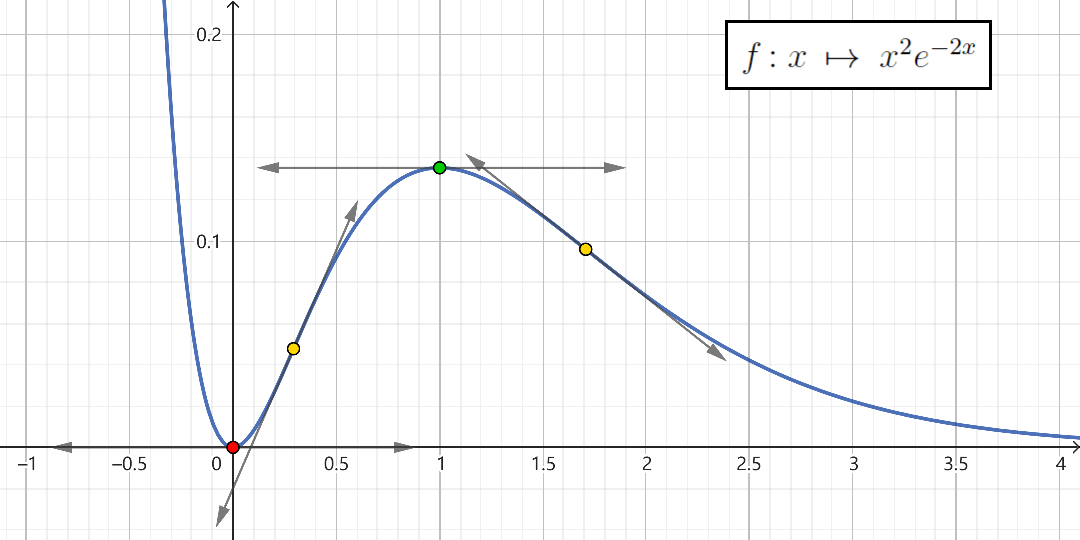
\includegraphics[width=0.8\textwidth]{tu/研究函数2.png}
\end{figure}

% \newpage  % 为了适应 研究函数2.png 的位置

\begin{sk}
    \mbox{} \\
    \indent 1. 怎样用函数的二次微变判定它是否严格上凸(下凸)?\\
    \indent 2. 在区间$I$上不连续的函数能否在$I$上凸或下凸?说明理由。
\end{sk}

\begin{xt}
    \mbox{} \\
    \indent 1. 判断以下函数的凸性:
    $$
    \begin{array}{ll}
        1. \quad x \mapsto x^5 + 10x^2 - 1 \qquad &2. \quad x \mapsto \tan{x} + 2\ln{cos{x}} \\
        3. \quad x \mapsto (x+1)\ln{\left(1 - \frac{1}{x}\right)} \qquad &4. \quad x \mapsto \left(1 - x^2\right)e^{-\frac{x^2}{2}}
    \end{array}
    $$
    \indent 2. 证明:如果函数下凸,那么对$I$中任意三点$x < z < y$,都有
    $$ \frac{f(z) - f(x)}{z - x} \leqslant \frac{f(y) - f(x)}{y - x}  \leqslant \frac{f(y) - f(z)}{y - z}. $$
    \indent 3. 函数$f$在区间$I$上可微且下凸。证明:$f$在$I$中任一点的切线总在$f$图像的下方。\\
    \indent 4. 证明\textbf{凸心不等式}:如果函数$f$在区间$I$下凸,那么对$I$中$n$个不同的数$x_1, x_2, \cdots , x_n$,
    以及大于等于零,和为$1$的$n$个系数$a_1, a_2, \cdots, a_n$,总有:
    $$ f\left(\sum_{i=1}^n a_i x_i\right) \geqslant \sum_{i=1}^n a_i f(x_i). $$
    \indent 5. 使用凸心不等式证明诸均值不等式。\\
    \indent 6. 证明,对任意$x\in\left(0; \frac{\pi}{2}\right)$,总有:
    $$ \frac{2}{\pi} x < \sin{x} < x.$$
    \indent 7. 已知$f$、$g$是从$\mathbb{R}$到$\mathbb{R}$的下凸函数,$g$单调递增。
    证明:复合函数$g\circ f$也是下凸函数。\\
    \indent 8. $f$、$g$是区间$I$上的下凸函数。定义函数:
    $$ f \wedge g : x \mapsto \left\{
        \begin{array}{cl}
            f(x) & \mbox{如果} f(x) > g(x) \\
            g(x) & \mbox{如果} f(x) \leqslant g(x) \\
        \end{array}
    \right.
    $$
    \indent 函数$f \wedge g$的值总是$f$、$g$中较大者。$f \wedge g$是否是下凸函数?\\
    \indent 如果定义函数$f \vee g$为$f$、$g$中较小者,$f \vee g$是否是下凸函数?

\end{xt}

\section{函数的零点}

函数的零点,是使得函数取值为$0$的点。换句话说,如果某个$a$使得$f(a) = 0$,就说$a$是函数$f$的零点。
函数$f$的零点就是方程$f(x) = 0$的解。

在科学研究和生产中,我们经常遇到这样的问题:对于有表达式的函数,如何知道它们是否有零点,或者零点的位置呢?

对于简单的函数,我们知道怎么求它们的零点。比如一次函数或二次函数,它们的零点对应一次方程和二次方程的根。

一种解决方法是通过研究$f$自身的性质,直接求方程$f(x) = 0$的解。
对于有表达式的函数$f$,有大量的研究探讨怎样把它的解用$f$的表达式和我们已知的函数表示出来。
这样的表示称为\textbf{显式解}或\textbf{解析解}。这样求出的解就是函数的零点确切的位置。

另一种思路则不追求找出零点确切的位置。很多时候,函数$f$十分复杂,难以求显式解。
而在研究和生产中,我们往往允许一定的误差。
因此,如果能通过简便的方法,找出和函数真正的零点位置“差不多”的值,也是很好的。
这样的值称为\textbf{数值解}或\textbf{近似解}。

举例来说,设有函数$f: x\mapsto x^3 - 2$,我们希望找出它的一个零点。

观察方程$x^3 = 2$,我们不难发现,通过开方运算,可以得到$x = \sqrt[3]{2}$。
这是方程$f(x) = 0$的一个显式解,它表示函数$f$零点的确切位置。

另外,如果事先约定一个允许的误差范围,比如$0.01$,我们也可以用逐步逼近的方法,估计函数的零点。
也就是找到令$|x - a| < 0.01$的$x$。

设零点为$a$。按照定义,$a^3 = 2$。考虑函数$x\mapsto x^3$,它在$\mathbb{R}$上严格单调递增,
因此,如果能找到$x_1^3 < 2 < x_2^3$,就说明$x_1 < a < x_2$。

我们从几个简单的值开始尝试:$0$、$1$、$2$,得到:$1^3 < 2 < 2^3$。因此$1 < a < 2$。
接下来不断使用二分法,$5$次之后,可以得到$1.25^3 < 2 < 1.265625^3$。
而$1.265625 - 1.25 < 0.02$,于是我们说$a$约等于两者的平均值,也就是$1.2578125$。
这个值和零点的确切值差距不会超过$0.02$的一半,也就是$0.01$。

从$1 < a < 2$出发,是否有更好的方法找到近似解呢?我们来看$f$的图像。
如果把零点$a$到$2$的函数图像近似考虑成直线,作$f$在$x=2$处的切线:
$$ y = \partial f(2)\cdot (x - 2) + f(2) $$
切线与$x$轴的交点
$$ x_1 = 2 - \frac{f(2)}{\partial f(2)} $$
就是零点。

\begin{figure}[h]
    \vspace{4pt}
    \centering
    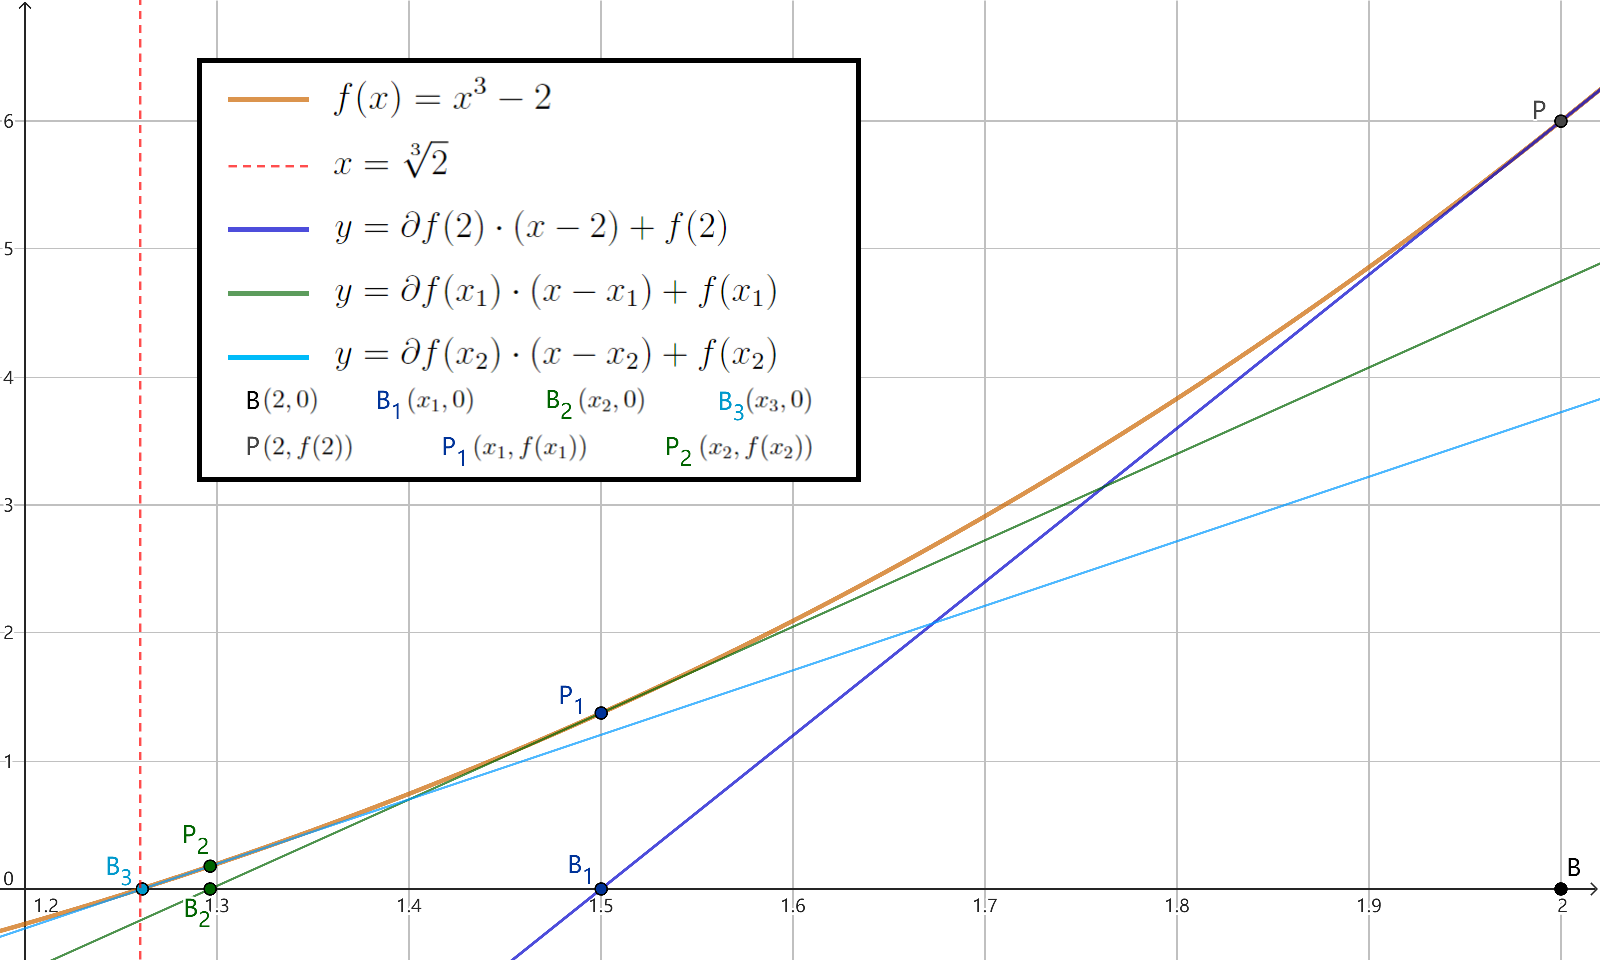
\includegraphics[width=\textwidth]{tu/切线法1.png}
\end{figure}

实际上,由于$f$的图像并不是直线,因此交点$x_1$和零点有一定的误差。
但我们可以继续从$x_1$出发,考虑$a$和$x_1$之间的函数曲线。
由于$a$和$x_1$距离更近了,因此这部分函数曲线更像直线了。
再次作$f$在$x=x_1$处的切线:
$$ y = \partial f(x_1)\cdot (x - x_1) + f(x_1) $$
它与$x$轴的交点
$$ x_2 = x_1 - \frac{f(x_1)}{\partial f(x_1)} $$
就更接近零点。
而我们如果继续从$x_2$出发,重复以上的做法,就能找到更接近零点的交点。

这种寻找零点近似解的方法称为\textbf{切线法}。

从$x=2$出发,可以找出交点$x_1 = 1.5$,$x_2 \approx 1.2963$,$x_3 \approx 1.2609$,$x_4 \approx 1.2599$,等等。

如何估计这些点和零点之间的误差呢?我们考虑第$n$次切线交点$x_n$和第$n+1$次切线的交点$x_{n+1}$。按定义:
$$ 0 = f(x_n) + \partial f(x_n)\cdot (x_{n+1} - x_n). $$
按零点的定义,把函数在$x_n$处展开:
$$ 0 = f(a) = f(x_n) + \partial f(x_n)\cdot (a - x_n) + \partial^2 f(c)\cdot (a - x_n)^2, $$
其中$c$是$a$和$x_n$之间的数。

从这两个式子可以推出:
$$ x_{n+1} - a = \frac{\partial^2 f(c)}{2\partial f(x_n)} (x_n - a)^2 = \frac{\partial^2 f(c)}{\partial f(x_n)} (x_n - a)(x_n - a),$$
即
$$ \frac{\left| x_{n+1} - a \right|}{\left| x_n - a \right|} = \left| \frac{\partial^2 f(c)}{2\partial f(x_n)} (x_n - a)\right|.$$

记上式右边的比例系数为$k_n =  \left|\frac{\partial^2 f(c)}{2\partial f(x_n)} (x_n - a)\right|$。如果$k_n$小于$1$,
$x_{n+1}$到$a$的距离就小于$x_n$到$a$的距离。

进一步说,如果$\left| x_{n+1} - a \right| < 0.5 \cdot \left| x_n - a \right|$,那么
\begin{align*}
    \left| x_{n+1} - x_n \right| &= \left| (x_{n+1} - a) - (x_n - a) \right| \\
    &\geqslant  \left| (x_n - a) \right| - \left| x_{n+1} - a \right| \\
    &> \left| x_{n+1} - a \right|.
\end{align*}
因此,只要观察到连续两次交点的距离小于误差,就可以确定最后一个交点和零点距离在误差范围内,取最后一个交点作为近似解即可。

下面来估计$k_n$的大小。

由于$c$和$x_n$都在区间$(1;1.5]$内,
而$\partial f: x\mapsto 3x^2$和$\partial^2 f: x\mapsto 6x$在区间内都是单调递增函数,因此总有$\partial^2 f(c) < 9$,
$\partial f(x_n) > 3$。因此不论$n$多大,总有$\frac{\partial^2 f(c)}{2\partial f(x_n)} < 1.5$。

$n=1$时,$|x_n - a| < 1.5 - 1 = 0.5$,所以
$$k_1 < 1.5 \times 0.5 = 0.75 < 1.$$
这说明,$|x_2 - a| < |x_1 - a|$,而这又告诉我们,
$$k_2 < 1.5 \cdot |x_2 - a| < 1.5 \cdot |x_1 - a| <0.75 < 1.$$

因此,用归纳法可知,不论$n$多大,总有$|x_{n+1} - a| < |x_n - a|$,$k_n < 1$。

进一步估计$k_2$。
$|x_2 - a| < x_2 - 1 < 0.3$,所以
$$ k_2 < 1.5 \cdot |x_2 - a| < 1.5 \times 0.3 < 0.5, $$
这说明$|x_3 - x_2| > |x_3 - a|$。同理,
$|x_3 - a| < 0.3$,所以$k_3 < 0.5$。因此$|x_4 - x_3| > |x_4 - a|$。
而$|x_4 - x_3| < 0.01$,因此,取$x_4 \approx 1.2599$为近似解,误差就小于$0.01$了。

与实际的零点对比,$1.2578125$的误差大约是千分之二,而$x_4$的误差小于百万分之一。

在大多数情况下,用好切线法,可以取得比二分法更好的效果。
但是,使用切线法也有前提条件,否则可能无法求出近似解。

首先,我们需要保证函数二次可微。其次,从上面的推导中可以看到,我们需要保证$k_n$总小于$1$,否则切线交点会离零点越来越远。
从$k_n$的构成来看,这就等于要求最初作切线的地方和零点不能距离太远,函数$f$在零点附近单调,而且微变率不能太小,而二次微变率不能太大。

综上所述,我们可以这样总结寻找二次可微函数零点近似解的方法:

\begin{center}
    \fbox{
        \shortstack[l]{
    1. 研究函数的单调和凹凸性,确定零点所在的区间。\\
    2. 如果零点在极值点附近,那么不适用切线法,使用\\
    \phantom{3. }二分法求零点。\\
    3. 在每个单调区间中使用二分法,把零点所在区间缩小\\
    \phantom{3. }到两端异号,且单调性和凹凸性都不变的区间。\\
    4. 调整零点所在区间,使得函数的二次微变最大值和\\
    \phantom{3. }微变最小值的比值乘以区间长度小于$2$。如果无法\\
    \phantom{3. }满足,则使用二分法。\\
    5. 如果函数在区间中上凸,那么以函数值小于零的一端\\
    \phantom{3. }为初始点;如果函数在区间中下凸,那么以函数值\\
    \phantom{3. }大于零的一端为初始点。\\
    6. 作过函数初始点的切线,与$x$轴交于一点$x_1$,\\
    \phantom{3. }如果$x_1$是零点则结束,否则以$x_1$为下一次的初始点。\\
    % \phantom{3. }\\
    7. 重复操作,并估计比例系数$k_n$,必要时可以调整初始\\
    \phantom{3. }点,以保持$k_n<1$。\\
    8. 如果$k_n<0.5$且$|x_{n+1} - x_n|$小于误差要求,则停止,\\
    \phantom{3. }以$x_{n+1}$为近似解。
        }
    }
\end{center}

\begin{sk}
    \mbox{} \\
    \indent 1. 以上$x^3 - 2$的例子中,能否从$x=1$处开始使用切线法?为什么?\\
    \indent 2. 如果把误差要求改为“使$|f(x)| < 0.01$”,会有什么不同?\\
    \indent 3. 如果把误差要求改为“两次估计值相差小于$0.01$”,会有什么不同?\\
    \indent 4. 如果函数在某段区间内有零点,在该区间内单调,但凹凸性变化了,能否对这段区间应用切线法?\\
    \indent 5. 二次不可微的可微函数,能否用切线法?如果不能,如何改进?连续但不可微的函数,能否用切线法?如果不能,如何改进?
\end{sk}

\begin{xt}
    \mbox{} \\
    \indent 1. 已知$\ln{2} \approx 0.7$,求函数$x\mapsto \ln{(x+1)} - 0.5$的一个零点,误差在$0.1$内。\\
    \indent 2. 求函数$x\mapsto 3\sin^2{x} - 1$的一个零点,误差在$0.1$内。\\
    \indent 3. 考虑函数$f:x\mapsto x^4-3 x^3-3 x^2+6 x-8$ \\
    \indent 3.1. 证明:函数$f$在区间$(2;+\infty)$上恰有一个极值点。并说明这个极值点的性质。\\
    \indent 3.2. 估计这个极值点的位置,误差在$0.01$内。
\end{xt}

% \section{曲线的性质}
% % 参数方程曲线的局部性质研究

\chapter{平直空间}
%将平面和立体空间扩展为一般的平直空间
平面和立体空间是我们熟悉的概念。为了讨论其中的点、线等形状,我们引入了向量的概念。
我们发现,除了实际中的空间,数学中还有别的概念,遵循和平面向量类似的法则。

\begin{ex}
    \mbox{} \\
    \indent 1. 设$\mathbb{K}$是某个数域(比如有理数集或实数集),考虑所有次数不超过$3$次的整式的集合:
    $$\mathbb{K}_3[x] = \{ax^3 + bx^2 + cx + d \, | \, a, b, c, d \in \mathbb{K}\}$$
    \indent 2. 考虑$S_2$是所有满足以下方程的实变函数的集合。
    $$ \partial^2 f + f = 0$$
\end{ex}

第一个例子里,集合$\mathbb{K}_3[x]$的每个元素都可以唯一表示成$\{1, x, x^2, x^3\}$的直组合。
如果我们把$\{1, x, x^2, x^3\}$看作“基底”,那么$\mathbb{K}_3[x]$中的元素就可以看成向量。

第二个例子里,考虑$S_2$中元素$u$、$v$的直组合$au + bv$:
$$ \partial^2 (au + bv) = a \partial^2 u + b \partial^2 v,$$
所以
\begin{align*}
    \partial^2 (au + bv) + au + bv &= a \partial^2 u + b \partial^2 v + au + bv  \\
    &= a(\partial^2 u + u) + b(\partial^2 v + v) = 0.  
\end{align*}
$au + bv$也是$S_2$中元素。
于是,我们也可以把$S_2$中元素看作向量。比如,可以验证正弦函数$\sin$和余弦函数$\cos$都是$S_2$中元素,
因此,其任意直组合$x\mapsto a\sin{x} + b\cos{x}$也是$S_2$中元素。

就像日常计数中抽象出数和代数的概念一样,通过研究这些问题和平面、立体空间的共通之处,
我们抽象出一种新概念,叫做\textbf{平直空间}。

\begin{df}
    给定作为系数的数域$\mathbb{K}$(如有理数或实数),$\mathbb{K}$上的\textbf{平直空间}$\mathbb{V}$是这样一个集合:

    首先,$\mathbb{V}$上定义了两种二元运算:$\diamond$和$\bullet$。其中:
    \begin{itemize}
        \item $\diamond$运算将两个$\mathbb{V}$中的元素映射为$\mathbb{V}$中的另一个元素。
        \item $\bullet$运算将一个$\mathbb{K}$中的元素和一个$\mathbb{V}$中的元素映射为$\mathbb{V}$中另一个元素。
    \end{itemize}
    其次,$\mathbb{K}$、$\mathbb{V}$和以上两种运算具有以下七种性质:
    \begin{enumerate}
        \item $\mathbb{V}$中元素对于$\diamond$运算满足交换律:
        $$\forall \,\, \mathbf{u}, \, \mathbf{v} \, \in \mathbb{V}, \,\, \mathbf{u} \diamond \mathbf{v} = \mathbf{v} \diamond \mathbf{u}.$$
        \item $\mathbb{V}$中元素对于$\diamond$运算满足结合律:
        $$\forall \,\, \mathbf{u}, \, \mathbf{v}, \, \mathbf{w} \, \in \mathbb{V}, \,\, (\mathbf{u} \diamond \mathbf{v}) \diamond \mathbf{w} = \mathbf{u} \diamond (\mathbf{v} \diamond \mathbf{w}).$$
        \item $\mathbb{V}$中元素对于$\diamond$运算存在零元素:
        $$\exists \,\, \mathbf{0} \, \in \mathbb{V} \mbox{,使得}\,\,\, \forall \,\, \mathbf{u} \, \in \mathbb{V}, \,\, \mathbf{u} \diamond \mathbf{0} = \mathbf{u}.$$
        \item $\mathbb{K}$中有$\bullet$运算的单位元$1_{\mathbb{V}}$:
        $$\forall \,\, \mathbf{u} \, \in \mathbb{V}, \,\,\, 1_{\mathbb{V}} \bullet \mathbf{u} = \mathbf{u}. $$
        % \item $\mathbb{V}$中元素对于$\diamond$运算存在逆元素:$\forall \,\, \mathbf{u} \, \in \mathbb{V}, \,\,\, \exists \,\, \mathbf{v} \, \in \mathbb{V}$ 使得 $\mathbf{u} \diamond \mathbf{v} = \mathbf{0}.$
        \item $\mathbb{K}$中乘法$\cdot$和$\bullet$运算兼容:
        $$\forall \,\, a, \, b \, \in \mathbb{K}, \,\,\, \forall \,\, \mathbf{u} \, \in \mathbb{V}, \,\, (a \cdot b)\bullet\mathbf{u} = a \bullet (b\bullet\mathbf{u}).$$
        \item $\bullet$运算对$\mathbb{K}$中加法$+$满足分配律:
        $$\forall \,\, a, \, b \, \in \mathbb{K}, \,\,\, \forall \,\, \mathbf{u} \, \in \mathbb{V}, \,\,\, (a + b)\bullet\mathbf{u} = (a \bullet \mathbf{u}) + (b \bullet \mathbf{u}). $$
        \item $\mathbb{K}$中乘法$\cdot$对$\diamond$运算满足分配律:
        $$\forall \,\, \mathbf{u}, \, \mathbf{v} \, \in \mathbb{V}, \,\,\, \forall \,\, a \, \in \mathbb{K}, \,\,\, a\cdot(\mathbf{u} \diamond \mathbf{v}) = (a \cdot \mathbf{u}) \diamond (a \cdot \mathbf{v}). $$
    \end{enumerate}
\end{df}

以上的定义可能比较难理解。我们可以比照平面、立体空间的向量来逐步分析。

以平面向量为例,作为系数的数域$\mathbb{K}$就是实数域$\mathbb{R}$。
两种二元运算:$\diamond$和$\bullet$分别就是向量的加法和数乘。

这样看来,七种性质的前三种和平面向量是一样的。
第五、六种性质就是平面向量定义中的“放缩和四则运算相容”。
第七种性质就是平面向量定义中的“放缩和平移相容”。

总体来说,平直空间的定义是从平面、立体空间的向量衍生而来。
新增的第四种性质是保证空间的尺度不变:乘以系数$1$不会改变向量的大小。

可以验证,前面的两个例子:$\mathbb{K}_3[x]$和$S_2$,都是平直空间。

一般来说,对任意正整数$n$,由次数不超过$n$的整式构成的集合:
$$ \mathbb{K}_n[x] = \{a_0 + a_1 x + \cdots + a_n x^n \, | \, a_0, a_1, \cdots , a_n \in \mathbb{K}\} $$
是平直空间。所有整式的集合$\mathbb{K}[x]$也是平直空间。

给定整式$P(x) = a_0 + a_1 x + \cdots + a_n x^n$,它可以对应以下的方程:
$$ a_0 f + a_1 \partial f + \cdots + a_n \partial^n f = 0. $$
这个方程所有解的集合$S_P$也是平直空间。

方便起见,平直空间的元素,也称为向量。对应的二元运算也称为加法、数乘。
其他的概念也沿用平面、立体空间中的称呼。

\begin{xt}
    \mbox{} \\
    \indent 1. 证明:零向量只有一个,任何向量乘$0$得到零向量。\\
    \indent 2. 证明:零向量乘任何数得到零向量。\\
    \indent 3. 证明:任何向量$\mathbf{a}$都有唯一的反向量$\mathbf{b}$,满足$\mathbf{a} + \mathbf{b} = \mathbf{0}$。\\
    \indent 4. 实数集是否是平直空间?有理数集、整数集呢?数轴上的区间是否是平直空间?\\
    \indent 5. 给定正整数$n$,由次数为$n$的整式构成的集合是否是平直空间?\\
    \indent 6. 所有有理数列的集合$\mathbb{Q}^\mathbb{N}$是否是平直空间?\\
    \indent 7. 所有奇函数的集合是否是平直空间?所有偶函数的集合呢?\\
    \indent 8. 所有有序数组$(a, b, c, d)$(其中元素为实数)的集合是否是平直空间?\\
    \indent 9. 所有在区间$[0;1]$上连续的函数的集合是否是平直空间?所有有界函数的集合是否是平直空间?\\
    \indent 10. 所有在区间$[0;1]$上$3$次可微的函数的集合是否是平直空间?\\
    \indent 11. 平面中的直线是否是平直空间?立体空间中的平面是否是平直空间。
\end{xt}

\section{子空间与和空间}
看了各种各样的平直空间,我们来了解它们之间的关系。

首先,我们想知道平直空间的子集是否是平直空间。
如果看平面和立体空间的例子,我们会发现,平面、立体空间的子集中,
有些满足平直空间的定义,另一些则不满足。比如,可以验证,平面中,过原点的直线是平直空间,不过原点的不是;
立体空间中,过原点的平面和直线是平直空间,不过原点的平面和直线不是平直空间。

直觉上,平直空间的子集里的元素也是满足向量的性质的,
唯一的问题是:子集中的向量运算后是否还在子集中。
只要这一点能够满足,平直空间的子集应该就是平直空间了。

\begin{df}{\textbf{子空间}}
    平直空间的非空子集,如果(关于空间的运算)仍然是平直空间,就称为该平直空间的\textbf{子空间}。
    其中,不等于平直空间自身的子空间称为该平直空间的\textbf{真子空间}。
\end{df}

\begin{tm}
    平直空间的非空子集,如果关于空间的运算封闭(也就是说,子集的元素经过运算后仍在子集中),
    就是子空间。
\end{tm}

显然,由于运算不变,平直空间子集的元素自动满足运算法则。唯一需要验证的是零向量也在子集里。
这就要由运算封闭的性质来保证。对子集中元素$\mathbf{u}$,
零向量可以写成$\mathbf{u} - \mathbf{u}$,因此根据封闭性质,还在子集中。

用这个方法,可以验证$\mathbb{Q}_n[x]$是$\mathbb{R}[x]$的子空间,
如果正整数$n<m$,那么$\mathbb{Q}_n[x]$是$\mathbb{R}_m[x]$的子空间。

对于立体空间来说,过原点的平面是它的子空间,而过原点的直线是它的子空间,
也是包含它的平面的子空间。可以证明:

\begin{tm}
    给定平直空间$\mathbb{V}$,$\mathbb{V}$的两个子空间的交集仍然是$\mathbb{V}$的子空间。
\end{tm}

所有子空间的交集是$\{\mathbf{0}\}$,它是任何平直空间都会有的子空间。我们也说它是\textbf{平凡}的。

子空间的并集是否是子空间呢?比如,两个过原点的平面,并集是否是子空间呢?
一般来说并不是,并集无法对向量的运算法则封闭。可以发现,并集要成为子空间的话,需要“更多的”向量。
为此,我们引入类似于并集的概念。

\begin{df}{\textbf{和空间}}
    \mbox{} \\
    给定平直空间$\mathbb{V}$以及它的两个子空间$\mathbb{U}_1$、$\mathbb{U}_2$,
    $\mathbb{U}_1$、$\mathbb{U}_2$的\textbf{和空间}是:
    $$ \{ \mathbf{u}_1 + \mathbf{u}_2\,|\, \mathbf{u}_1 \in \mathbb{U}_1,\,\,\, \mathbf{u}_2 \in \mathbb{U}_2\}.$$
    记作$\mathbb{U}_1 + \mathbb{U}_2$。
\end{df}
可以验证,这样定义的和空间也是平直空间$\mathbb{V}$的子空间。

子空间的和满足结合律和交换律。用归纳法不难得出,平直空间的有限个子空间也可以定义和空间。

给定立体空间的两个子空间:过原点的直线$\mathbb{R}\mathbf{v}_1$、$\mathbb{R}\mathbf{v}_2$,
它们的和空间就是$\mathbb{R}\mathbf{v}_1 + \mathbb{R}\mathbf{v}_2$。
如果$\mathbf{v}_1$、$\mathbf{v}_2$不共轴,那么和空间是平面,否则是直线。

给定立体空间的两个子空间:过原点的直线$\mathbb{R}\mathbf{v}_1$与平面$\gamma: \mathbb{R}\mathbf{v}_2 + \mathbb{R}\mathbf{v}_3$,
它们的和空间就是$\mathbb{R}\mathbf{v}_1 + \mathbb{R}\mathbf{v}_2 \mathbb{R}\mathbf{v}_3$。
如果$\mathbf{v}_1$在$\mathbb{R}\mathbf{v}_2 + \mathbb{R}\mathbf{v}_3$中,那么和空间就是$\gamma$。
否则,和空间就是整个空间。

给定立体空间的两个子空间:过原点的平面$\gamma_1: \mathbb{R}\mathbf{u}_1 + \mathbb{R}\mathbf{v}_1$、$\gamma_2: \mathbb{R}\mathbf{u}_2 + \mathbb{R}\mathbf{v}_2$,
它们的和空间是$\mathbb{R}\mathbf{u}_1 + \mathbb{R}\mathbf{v}_1 + \mathbb{R}\mathbf{u}_2 + \mathbb{R}\mathbf{v}_2$。
如果$\gamma_2$中有不在$\gamma_1$中的向量,那么和空间是整个空间。
否则,和空间就是$\gamma_1$。

如果平直空间$\mathbb{V} = \mathbb{U}_1 + \mathbb{U}_2$,且
$\mathbb{U}_1 \cap \mathbb{U}_2 = \{\mathbf{0}\}$,就说$\mathbb{V}$
是$\mathbb{U}_1$、$\mathbb{U}_2$的\textbf{直和},记作。
$$\mathbb{V} = \mathbb{U}_1 \oplus \mathbb{U}_2.$$
要注意的是,这里的$\oplus$只是记录两个子空间交集为$\{\mathbf{0}\}$的性质,并不是一种运算。

\begin{sk}
    \mbox{} \\
    \indent 1. 子空间的交集、和空间,与子集的交集、并集有什么相似之处?有没有类似空集的概念?\\
    \indent 2. 能否定义子空间“不相交”?能否把平直空间用子空间划分?\\
    \indent 3. $\mathbb{Q}_3[x]$是$\mathbb{R}_3[x]$的子空间吗?$\mathbb{Q}^\mathbb{N}$是$\mathbb{R}^\mathbb{N}$的子空间吗?
\end{sk}

\begin{xt}
    \mbox{} \\
    \indent 1. 给出以下平直空间的(非平凡的)子空间的例子。\\
    $$
    \begin{array}{ll}
        1. \quad \mathbb{R}_3[x] & \qquad 2. \quad \{f: \mathbb{R} \rightarrow \mathbb{R} \, | f(0) = 0, \,\,\, f(1) = 0\} \\
        3. \quad \{f \, | \, \partial^3 f = f\} & \qquad 4. \quad \{(a, b, c) \, | \, a, b, c \in \mathbb{R}\} \\
        5. \quad \mathbb{R}^\mathbb{N} & \qquad 6. \quad \{f: [0;1] \rightarrow \mathbb{R} \, | \, f \mbox{可微,且} \partial f(0.5) = 0\}
    \end{array}
    $$
    \indent 2. 设有立体空间中的向量$(1, 0, 0)$、$(0, 1, -1)$。求包含它们的最小子空间。\\
    \indent 3. 证明:如果非常数整式$Q$是$P$的因式,那么$S_Q$是$S_P$的子空间。\\
    \indent 4. 证明:如果$\mathbb{U}_1$、$\mathbb{U}_2$是$\mathbb{V}$的子空间,
    那么$\mathbb{U}_1 + \mathbb{U}_2$是$\mathbb{V}$的子空间。\\
    \indent 5. 证明:$\mathbb{V}$平直空间能写成两个子空间$\mathbb{U}_1$、$\mathbb{U}_2$的直和,
    当且仅当$\mathbb{V}$中任意元素都能以唯一的方式写成$\mathbb{U}_1$中元素与$\mathbb{U}_2$中元素的和。
\end{xt}

\section{生成空间}
以上的章节中,我们已经认识到,平直空间是一种特殊的集合。给定集合,我们可以将它补充成平直空间。
\begin{df}{\textbf{生成空间}}
    给定系数域为$\mathbb{K}$的平直空间$\mathbb{V}$的子集$A$,它的\textbf{生成空间}是\footnote{如果没有强调$A$是哪个平直空间的子集,一般来说,要约定系数域$\mathbb{K}$。我们约定:如果没有强调,系数域一般是实数集$\mathbb{R}$。}:
    $$ \vect{A} = \left\{\left. \sum_{i=1}^n a_i \mathbf{u}_i \, \right| \, n\in\mathbb{Z}^+, \,\,\, \forall 1\leqslant i \leqslant n \,\,\, a_i \in \mathbb{K}, \,\,\, \mathbf{u}_i \in \mathbb{V} \, \right\} $$
    即考虑集合中有限个元素的直组合,所有这样的直组合的集合就是它的生成空间。
    
    反之,如果某个集合$A$的生成空间是平直空间$\mathbb{U}$,就说$A$是$\mathbb{U}$的\textbf{生成集}。

    约定空集的生成空间是平凡空间$\{\mathbf{0}\}$。
\end{df}

显然,集合$A$的生成空间是它的母集。

容易看出,如果某个平直空间包含集合$A$,那么肯定也包含$A$的生成空间。
因此,$A$的生成空间是所有包含$A$的平直空间的子空间。
换句话说,$A$的生成空间是包含$A$的最小的平直空间。

作为推论,不难得出:平直空间的生成空间就是自己。

根据定义可以给定集合$A$、$B$,那么:
\begin{itemize}
    \item 如果$A\subset B$,那么$\vect{A}$是$\vect{B}$的子空间。
    \item $\vect{A\cap B}$是$\vect{A}\cap\vect{B}$的子空间。
    \item $\vect{A\cup B} = \vect{A} + \vect{B}$。
\end{itemize}

可以注意到,$A$中元素是否重复,不妨碍定义它的生成空间。
因此,我们可以定义“允许元素重复的集合”:
\begin{df}{\textbf{族}}
    \mbox{} \\
    设$A$为集合,在$A$中可重复地抽取元素,放在一起,称为\textbf{族}。族可以是有序的。
\end{df}
我们可以把生成空间的概念扩大到向量族的生成空间。
这样定义的生成空间也有以上提到的基本性质。

如果某个平直空间能通过有限个向量生成,就说它是\textbf{有限生成空间}。
比如,$\mathbb{R}_3[x]$就是有限生成空间,因为每个向量都是$\{1, x, x^2, x^3\}$的直组合。
可以验证
$$\mathbb{R}_3[x] = \vect{\{1, x, x^2, x^3\}}.$$
而$\mathbb{R}[x]$就不是有限生成空间。考虑$\mathbb{R}[x]$中$n$个元素,设它们之中最高的次数是$m$,
那么它们的直组合的次数不会超过$m$,因此无法生成次数大于$m$的整式。

平面和立体空间的基本定理说明,它们都是有限生成空间。

\begin{sk}
    \mbox{} \\
    \indent 1. 给定集合$A$、$B$,$\vect{A\cap B} = \vect{A}\cap\vect{B}$成立吗?\\
    \indent 2. 所有$[0;1]$上的连续函数的集合,是否是有限生成空间?
\end{sk}

\begin{xt}
    \mbox{} \\
    \indent 1. 求实系数多项式集合$\{x, 4x^3\}$的生成空间。\\
    \indent 2. 设$E$是$(1, \,\,2, \,\,0)$、$(0, \,\,-1, \,\,1)$生成的空间。
    把$E$写成一次方程的解集的形式,求该一次方程。\\
    \indent 3. 求$\{(x,\,\,y,\,\,z)\in\mathbb{R}^3 \, | \, x + 2y + z = 0 \}$的生成集。
    
\end{xt}

\section{基底和维数}

如果我们考虑$1,x,x^2$这三个向量,
它们生成的空间是$\mathbb{R}_2[x]$。
那么$1,x,2x-1,x^2$这四个向量呢?它们生成的空间仍然是$\mathbb{R}_2[x]$。

我们可以发现,相比$1,x,x^2$,加入$2x-1$这个向量,有点“多余”。为什么呢?
因为$2x-1$本身就是$1, x$的直组合,加入之后并不能“贡献”什么新的东西。

容易发现,用足够多的向量来生成空间并不是难事。比如,空间$\mathbb{V}$自己肯定可以生成$\mathbb{V}$。
所以,我们比较关心的是最小生成集的问题,即:生成空间$\mathbb{V}$,最少要用多少个向量?

平面和立体空间的基本定理说明,生成平面至少要两个向量,生成立体空间至少要三个向量。

直觉上来看,向量个数增多会让它们“更相关”,数量减少则使它们更“不相关”。
对平直空间来说,如果$A$是它的生成集,$B$是空间中一组直无关的向量,那么前者的元素应该比后者多。

可以证明(见附录$D$):
\begin{tm}\label{tm:4-3-10}
    有限生成空间中,任何一族直无关的向量,向量的个数都不多于任意一个生成族的向量个数。
\end{tm}
这是一个重要的结论。它告诉我们,有限生成空间中直无关的向量,个数有上限。
因此,平直空间的最小生成族也就是最大的直无关族。

\begin{df}{\textbf{平直空间的基底}}
    平直空间的\textbf{基底},就是它的直无关的生成族。基底的向量称为\textbf{基向量}。
\end{df}

这个定义和我们已经定义过的平面、立体空间的基底是一致的。

$\mathbb{R}_3[x]$的一个基底是$(1, x, x^2, x^3)$。
一般来说,$(1, x, \cdots, x^n)$是$\mathbb{R}_n[x]$的基底。

和平面、立体空间一样,平直空间的基底也满足:
\begin{tm}{\textbf{向量的唯一分解}}\label{tm:4-3-20}
    $ \mathcal{B} = (\mathbf{e}_1, \mathbf{e}_2, \cdots , \mathbf{e}_n )$是平直空间$\mathbb{V}$的一组基,
    当且仅当空间中每个元素$\mathbf{u}$都能以唯一的方式写成
    $$ \mathbf{u} = a_1\mathbf{e}_1 +a_2 \mathbf{e}_2 + \cdots + a_n\mathbf{e}_n, \,\,\, a_1,\,a_2,\,\cdots,\, a_n \,\in\,\mathbb{F}.$$
    称为$\mathbf{u}$的$\mathcal{B}$\textbf{分解}。$a_1, a_2, \cdots a_m$称为$\mathbf{u}$(在该分解下)的\textbf{分量}。
\end{tm}

有限生成空间必然有基底吗?直觉上,我们可以从空间的生成集出发,移除一些“多余”的向量,直到剩下的向量直无关为止。

\begin{tm}\label{tm:4-3-40}
    可以通过适当地移除元素,把有限生成空间$\mathbb{V}$的每个生成族变成基底。
\end{tm}

用具体的例子来说明。

$\left((1,0),(8,2),(3,1),(0,4),(0,0)\right)$是$\mathbb{R}^2$的生成集。

我们首先去除零向量,得到$\left((1,0),(8,2),(3,1),(0,4)\right)$。 
这组向量直相关:
$$ (8,2) = 2\cdot(1,0) + 2\cdot(3,1).$$
去除$(8,2)$,得到$\left((1,0),(3,1),(0,4)\right).$ 这组向量仍然直相关:
$$ (3,1) = 3\cdot(1,0) + 0.25\cdot(0,4).$$
去除$(3,1)$,得到$\left((1,0),(0,4)\right).$ 现在我们得到了一组直无关的向量,
而且能生成$\mathbb{R}^2$,即$\mathbb{R}^2$的一组基。

从上面的定理可以推出:
\begin{tm}\label{tm:4-3-50}
    任意有限生成空间都有基底。
\end{tm}

空间的基底就是最小生成集,因此大小应该相同。我们可以用定理\ref{tm:4-3-10}来证明。
选定同一空间的两个基底$\mathcal{B}_1$、$\mathcal{B}_2$,它们都是直无关的生成集。
根据定理\ref{tm:4-3-10},$\mathcal{B}_1$直无关,$\mathcal{B}_2$是生成集,
所以$|\mathcal{B}_1| \leqslant |\mathcal{B}_2|$。
同理可证,$|\mathcal{B}_2| \leqslant |\mathcal{B}_1|$。
因此$|\mathcal{B}_1| = |\mathcal{B}_2|$。

我们把有限生成空间$\mathbb{V}$基底的元素个数称为空间的\textbf{维数},记为$\dim \mathbb{V}$。
平直空间的维数是它的内禀性质,不依赖于附带的假设。

平面的维数是$2$,所以也常称为二维空间。立体空间维数是$3$,所以也称为三维空间。
过原点的直线作为子空间,维数是$1$,也称为一维空间。

由于有限生成空间必然有维数,我们也称其为\textbf{有限维空间}。

空间的任意生成集都可以缩减为它的基底。那么任意直无关的向量族能否扩充为基底呢?答案是肯定的。
\begin{tm}\label{tm:4-3-60}
    可以通过适当地添加元素,把有限生成空间$\mathbb{V}$的每一组直无关的向量变成基底。
\end{tm}

我们甚至有更具体的结论:
\begin{tm}\label{tm:4-3-70}
    给定有限生成空间$\mathbb{V}$的子空间$\mathbb{U}$,存在另一个子空间$\mathbb{W}$,使得
    $$ \mathbb{V} = \mathbb{U} + \mathbb{W}.$$
    且$\mathbb{U} \cap \mathbb{W} = \{\mathbf{0}\}$。
    $\mathbb{W}$称为子空间$\mathbb{U}$的\textbf{补空间},一般记作$\mathbb{U}^c.$
\end{tm}

这让我们联想到集合的补集。实际上,我们还可以证明:

\begin{tm}{\textbf{维数基本定理}}\label{tm:4-3-80}
    设$\mathbb{U}$和$\mathbb{W}$是有限维空间$\mathbb{V}$的两个子空间,则它们的维数满足以下关系:
    $$ \dim (\mathbb{U} + \mathbb{W}) = \dim \mathbb{U} + \dim \mathbb{W} - \dim (\mathbb{U} \cap \mathbb{W}).$$
\end{tm}
如果我们把空间的和比作集合的并,把空间的交比作集合的交,把空间的维数比作集合的元素个数,
则这个关系和有限集合的关系是一致的。

\begin{sk}
    \mbox{} \\
    \indent 1. 能否把$\mathbb{R}$看作系数域为$\mathbb{Q}$的平直空间?它是否是有限维空间?\\
    \indent 2. 基底中,基向量的排列顺序重要吗?按不同顺序排列的基向量,能否看做不同的基底?给出你的理由。
\end{sk}

\begin{xt}
    \mbox{} \\
    \indent 1. 说明以下结论:\\
    \indent 1.1. 有限维空间的生成集的元素个数不小于空间的维数。\\
    \indent 1.2. 有限维空间的直无关向量族的元素个数不小大于空间的维数。\\
    \indent 1.3. 有限维空间的生成集的元素个数等于空间的维数,则生成集是空间的基底。\\
    \indent 1.4. 有限维空间的直无关向量族的元素个数等于空间的维数,则直无关向量族是空间的基底。\\
    \indent 2. 给出$\{(x,\,\,y,\,\,z)\in\mathbb{R}^3 \, | \, x + 2y + z = 0 \}$的一个补空间。\\
    \indent 3. 请把$(1,\,\,1, \,\,1)$、$(0,\,\, -1, \,\,1)$扩充为$\mathbb{R}^3$的基底。\\
    \indent 4. 设二次可微函数$f:\mathbb{R} \rightarrow \mathbb{R}$是方程$\partial^2 f + f = 0$的解,
    并且$f(0) = \partial f(0) = 0$。\\
    \indent 4.1. 对任意$x$,证明:存在$0$与$x$之间的数$c$,使得
    $$ f(x) = -\frac{f(c)x^2}{2}. $$
    \indent 4.2. 设$M$是$|f|$在$[0;1]$上的最大值。证明$M \leqslant \frac{M}{2}$,从而$M = 0$。\\
    \indent 4.3. 证明$f$恒等于$0$。\\
    \indent 5. 设$S_2$为满足方程$\partial^2 f + f = 0$的实变函数的集合。\\
    \indent 5.1. 证明:如果$f,g\in S_2$满足$f(0) = g(0)$,$\partial f(0) = \partial g(0)$,那么$f = g$。\\
    \indent 5.2. 分别找出$S_2$中满足$f(0) = 0, \,\,\, \partial f(0) = 1$以及$f(0) = 1, \,\,\, \partial f(0) = 0$的函数$f_1$、$f_2$。\\
    \indent 5.3. 证明:$\{f_1, f_2\}$是$S_2$的基底。给出$S_2$的维数。
\end{xt}

\chapter{级数}
研究可微函数时,我们讨论过分析函数在某点附近的行为的问题。
我们的研究方法是:把函数在该点附近表示成多项式的形式。换句话说,我们把函数表示成一系列简单函数的和。
比如,指数函数在$0$附近可以写成:
$$e^x = 1 + x + \frac{x^2}{2} + \frac{x^3}{6} + \cdots + \frac{x^n}{n!} + \olim{x^n}.$$
那么,我们能不能把$e^x$直接写成无穷多个简单函数的和呢?

具体来说,对于每个$x$,我们能不能说,$e^x$就是把“所有”$\frac{x^n}{n!}$这样的项加起来的和呢?

我们并未定义过“无穷多个数的和”。不过,这个问题可以转化成一个数列的问题。
学习数列的时候,我们研究了趋于极限或趋于无穷的数列。
上面的问题,换句话说,就是问数列:
$$ 1, 1+x, 1+x + \frac{x^2}{2}, \cdots , 1 + x + \frac{x^2}{2} + \frac{x^3}{6} + \cdots + \frac{x^n}{n!}, \cdots $$
有没有极限。

传统上,我们把这样的数列用另一种方式表示,称为\textbf{级数}。

\begin{df}{\textbf{级数}}
    \mbox{} \\
    给定数列$\{a_n\}_{n\in\mathbb{N}}$,表达式:
    $$ a_0 + a_1 + a_2 + \cdots + a_n + \cdots $$
    称为数列$\{a_n\}$的\textbf{级数},简记为$\sum_{n\in\mathbb{N}} a_n$或$\sum a_n$。
    $a_n$称为\textbf{级数的通项},$\{a_n\}_{n\in\mathbb{N}}$也称为级数的\textbf{通项数列}。
    
    如果$\{a_n\}$的部分和序列:
    $$ a_0, a_0 + a_1, \cdots , \sum_{i=0}^n a_i, \cdots $$
    有极限,就说\textbf{级数收敛},其极限称为\textbf{级数和},记作:
    $$ \sum_{i=0}^\infty a_i $$
    否则说\textbf{级数发散}。
    
\end{df}

对于数列$\left\{\frac{x^n}{n!}\right\}_{n\in\mathbb{N}}$来说,它的级数就是
$$ 1 + x + \frac{x^2}{2} + \frac{x^3}{6} + \cdots $$
这个级数是否收敛,收敛的话,级数和是否是$e^x$,就是我们希望研究的内容。

\section{正项级数}

如果级数的通项都是正数或非负数,那么就说级数是\textbf{正项级数}。

正项级数是最方便研究的级数。对一般级数的研究,经常会转化到正项级数。

正项级数的部分和序列是单调递增数列。我们知道,单调递增数列要么有极限,要么趋于正无穷。
这两种情况分别对应级数收敛、级数发散。

举例来说,级数$\sum 2^{-n}$是正项级数。它的部分和$H_n$为:
$$ H_n = 1 + \frac{1}{2} + \cdots + \frac{1}{2^n}.$$
它的通项数列是无穷递缩等比数列,因此$H_n = 2 - 2^{-n}$。部分和序列$\{H_n\}$趋于$2$。
我们说级数$\sum 2^{-n}$收敛,级数和是$2$。

同理,级数$\sum r^{-n}$的部分和$H_n$为
$$ H_n = 1 + \frac{1}{r} + \cdots + \frac{1}{r^n} = \frac{1 - r^{-n-1}}{1 - r^{-1}}.$$
因此,$r>1$时,部分和序列$\{H_n\}$趋于$\frac{r}{r - 1}$,级数和是$\frac{r}{r - 1}$。

研究级数收敛,和研究数列收敛,有什么不同呢?实际上,级数是研究数列收敛性质的工具。

研究数列$\{a_n\}$是否收敛时,我们发现,将数列相邻项作差:
$$ a_0, a_1 - a_0, a_2 - a_1, \cdots $$
这样得到的数列的性质,对研究数列是否收敛更有用。我们把作差得到的数列称为原数列的\textbf{差分数列}。
可以验证,数列$\{a_n\}$的差分数列的部分和为:
$$ H_n = a_0 + (a_1 - a_0) + (a_2 - a_1) + \cdots + (a_n - a_{n-1}) = a_n. $$
也就是说,\textbf{数列的差分数列的级数,就是原数列}。

因此,研究数列是否收敛,就看它的差分数列,研究差分数列的级数是否有级数和。
如果差分数列有级数和,那么级数和就是原数列的极限。

\begin{sk}
    \mbox{} \\
    \indent 1. 通过差分数列来研究数列性质的方法,
    与通过研究函数的微变率、微变函数来研究函数性质的方法,有哪些共同之处?有哪些不同之处?
\end{sk}

\section{正项级数的收敛}
那么,怎样的正项级数收敛呢?

首先来看级数$\sum \frac{n}{n+1}$。这个级数的通项$\frac{n}{n+1}$趋于$1$。
也就是说,$n$足够大时,每增加一项,就等于给部分和加$1$。这样看来,级数不收敛。

下面严格来说明,由于
$$\lian{n\to +\infty }\frac{n}{n+1} = 1,$$
因此,对于$0<r<1$,总存在正整数$N$,只要$n>N$,就有$\frac{n}{n+1} > 1 - r$。
于是,部分和$H_n$可以写成:
$$ H_n > H_N + (n - N) \cdot (1 - r).$$
而数列$\{(n - N) \cdot (1 - r)\}$趋于正无穷,所以部分和$H_n$也趋于正无穷。也就是说,级数$\sum \frac{n}{n+1}$发散。

从这个证明可以看出,只要正项级数的通项不收敛到$0$,就总会有比较大的项加到部分和里,
于是级数就会发散。我们将其总结为:
\begin{tm}
    如果正项级数的通项没有极限或极限不为零,那么级数发散。
\end{tm}
\begin{proof}
    设正项级数$\sum a_n$的通项数列不收敛到$0$,那么按照定义,存在$r>0$,使得对任意正整数$N$,
    总有$n > N$,让$a_n \geqslant r$。

    因此,我们可以找到第一个$n_1$,使得$a_{n_1} \geqslant r$。把$n_1$作为$N$,又可以找到$n_2 > n_1$,
    使得$a_{n_2} \geqslant r$。以此类推,我们可以找到$\{a_n\}$的子列,其中每个元素都大于等于$r$。

    考虑级数$\sum a_n$的部分和$H_n$,当$n$大于子列的第$m$个下标时,$H_n$就大于等于$mr$。因此,部分和趋于正无穷。
    这说明级数不收敛。
\end{proof}

如果通项数列$\{a_n\}$收敛到$0$,级数是否就收敛呢?

考虑级数$\sum \frac{1}{n+1}$,它的通项是$\frac{1}{n+1}$,因此趋于$0$。
但我们可以证明,级数$\sum \frac{1}{n+1}$不收敛。

考虑数列$\{\frac{1}{n+1}\}$的前$2^m$项,我们可以把它这样拆分:
\begin{align*}
    1 \, &\geqslant \, 1  \\
    \frac{1}{2} &\geqslant \frac{1}{2}  \\
    \frac{1}{3} + \frac{1}{4} &\geqslant 2 \cdot \frac{1}{4} = \frac{1}{2}  \\
    \frac{1}{5} + \frac{1}{6} + \frac{1}{7} + \frac{1}{8} &\geqslant 4 \cdot \frac{1}{8} = \frac{1}{2}  \\
    \vdots \qquad & \qquad \vdots  \\\
    \frac{1}{2^{m-1}+1} + \frac{1}{2^{m-1}+2} + \cdots + \frac{1}{2^{m}} &\geqslant 2^{m-1} \cdot \frac{1}{2^{m}} = \frac{1}{2}  
\end{align*}

因此,级数前$2^m$项的部分和大于等于$1 + \frac12 \cdot (m - 1) = \frac{m+1}{2}$。
这说明级数不收敛。

再看另一个级数:$\sum \frac{1}{(n+1)^2}$,它的通项是$\frac{1}{(n+1)^2}$,同样趋于$0$。
然而,我们可以证明,这个级数是收敛的。
这是因为对任意正整数$n$,
$$ \frac{1}{(n+1)^2} < \frac{1}{n(n+1)} = \frac{1}{n} - \frac{1}{n+1}.$$
因此,部分和$H_n$可以写为:
$$ H_n = 1 + \sum_{i=1}^n \frac{1}{(n+1)^2} < 1 + \sum_{i=1}^n \left(\frac{1}{n} - \frac{1}{n+1}\right) = 1 + 1 - \frac{1}{n+1} < 2. $$
部分和序列有界,因此收敛。

从上面的讨论可以顺便推出:级数$\sum \frac{1}{(n+1)^a}$在$a\geqslant 2$时收敛,在$a\leqslant 1$时发散。
直觉上理解,就是$\{\frac{1}{n+1}\}$收敛到$0$还不够快,导致部分和增长得太多;
而$\sum \frac{1}{(n+1)^2}$、$\sum r^{-n}$收敛得足够快,因此部分和始终有限。

怎样把“收敛得足够快”这件事用严谨的方式说明呢?比照无穷的阶的形式,我们来考虑通项数列相邻两项的比值:
$$ q_n = \frac{a_n}{a_{n+1}} $$
直觉来说,如果$q_n$趋于某个小于$1$的数,那么$\{a_n\}$大体来说是增长的,不收敛到$0$,于是级数发散。
如果$q_n$趋于某个大于$1$的数$r$,那么$a_n$收敛到$0$,而且收敛得大致和$r^{-n}$一样快,于是级数收敛。

不过,对级数$\sum \frac{1}{n+1}$、$\sum \frac{1}{(n+1)^2}$,比值$\{q_n\}$都收敛到$1$。
因此,需要更细致的分析。遵循研究函数局部性质的思路,我们可以把它展开:
$$ q_n = 1 + \frac{t_1}{n} + \frac{t_2}{n^2} + \cdots $$
级数$\sum \frac{1}{n+1}$对应$t_1 = 1$,而$\sum \frac{1}{(n+1)^2}$对应$t_1 = 2$。

我们把$q_n$写成
$$ q_n = 1 + \frac{t_1}{n} + \olim{\frac{1}{n}}. $$
也就是:
$$ n(q_n - 1) = t_1 + \olim{1}.$$
即$n(q_n - 1)$趋于$t_1$。

如果$t_1 < 1$,那么按照极限的定义,总有$N$和$r<1$使得$n>N$时总有:$n(q_n - 1) < r$,即:
$$ na_n - (n+1)a_{n+1} < 0. $$
即$n>N$后,数列$\{na_n\}$单调递增。因此$a_n > \frac{Na_N}{n}$。
于是,级数$\sum a_n$的部分和增长得比$Na_N\sum \frac{1}{n}$快,因此发散。

如果$t_1 > 1$,那么按照极限的定义,总有$N$和$r>1$使得$n\geqslant N$时总有:$n(q_n - 1) > r$,
即
$$ na_n - (n+1)a_{n+1} \geqslant (r - 1)a_{n+1}.  $$
同理,可以写出:
\begin{align*}
    (n-1)a_{n-1} - na_n &\geqslant (r - 1)a_{n}  \\
    (n-2)a_{n-2} - (n-1)a_{n-1} &\geqslant (r - 1)a_{n-1}  \\
    \vdots \quad &\geqslant \quad \vdots  \\
    Na_{N} - na_n &\geqslant (r - 1)a_{N+1} 
\end{align*}
以上等式分边相加,就得到:
$$ Na_{N} \geqslant Na_{N} - na_n \geqslant (r - 1)\sum_{i=N+1}^n a_i. $$
于是部分和$H_n$可以写成:
$$ H_n \leqslant H_N + Na_{N}.$$
这说明级数收敛。

$t_1 = 1$时,需要更精细的分析,这里就不继续展开了。我们把以上的内容总结一下:

记正项级数$\sum a_n$的通项数列相邻两项的比值为:
$$ q_n = \frac{a_n}{a_{n+1}} $$
如果在$n$足够大的时候,总有以下情况,则可以做出正项级数是否收敛的判断。
\begin{enumerate}
    \item 如果$q_n$总大于某个大于$1$的数,那么级数收敛;
    \item 如果$q_n$总小于某个小于$1$的数,那么级数发散;
    \item 如果$q_n$可以写成$1 + \frac{A}{n} + \olim{\frac{1}{n}}$,且$A > 1$,那么级数收敛;
    \item 如果$q_n$可以写成$1 + \frac{A}{n} + \olim{\frac{1}{n}}$,且$A < 1$,那么级数发散。
\end{enumerate}

来看一些具体的例子。

级数$\sum \frac{1}{n!}$收敛,因为
$$\forall n \geqslant 1,  \,\,\,q_n = \frac{(n+1)!}{n!} = n+1 \geqslant 2. $$

$x>0$时,级数$\sum \frac{x^n}{n!}$收敛,因为
$$\forall n \geqslant x,  \,\,\,q_n = \frac{x^n (n+1)!}{n! x^{n+1}} = \frac{n+1}{x} \geqslant 1 + \frac{1}{x}. $$


$x>1$时,级数$\sum \frac{n^k}{x^n}$收敛,因为
$$\forall n \geqslant 1,  \,\,\,q_n = \frac{n^k x^{n+1}}{x^n (n+1)^{k}} = x\left(1 + \frac{1}{n}\right)^{-k}. $$
而数列$\left\{\left(1 + \frac{1}{n}\right)^k\right\}$趋于$1$,因此$q_n$趋于$x>1$。

级数$\sum n^a$的收敛情况跟$a$有关。比值$q_n = \left(1 + \frac{1}{n}\right)^{-a}$。
\begin{itemize}
    \item 如果$a\leqslant 0$,那么级数发散。
    \item 如果$a<0$,那么$q_n = \left(1 + \frac{1}{n}\right)^{-a} = 1 - \frac{a}{n} + \olim{\frac{1}{n}}$。
    \item 如果$-1 < a < 0$,那么级数发散。
    \item 如果$a = -1$,那么级数发散。
    \item 如果$a < -1$,那么级数收敛。
\end{itemize}

\begin{sk}
    \mbox{} \\
    \indent 1. 看了研究级数收敛性质的方法,对你研究函数的性质,有什么启发?\\
    \indent 2. 如果数列从某一项开始都是正数,这样的数列能否通过研究正项级数来讨论收敛性?
    进一步来说,数列的负项如果更多的话,如何转为正项级数来研究?
\end{sk}

\begin{xt}
    \mbox{} \\
    \indent 1. 以下级数是否收敛?说明原因。
    $$
    \begin{array}{ll}
        1. \quad \sum \frac{2}{n^2 - 3n + 3} \qquad &2. \quad \sum \frac{n!}{n^n} \\
        3. \quad \sum \frac{1}{\sqrt{n + 1}} \qquad &4. \quad \sum \frac{4^n (n!)^2}{(2n + 1)!} 
    \end{array}
    $$
    \indent 2. 给定$x>0$,证明:级数$\sum \frac{x^n}{n!}$收敛,级数和为$e^x$。\\
    \indent 3. 考虑正项级数$\sum a_n$。如果有正数列$\{B_n\}$,正数$c$,以及正整数$N$,使得
    $$ \forall n > N, \,\,\, B_n \frac{a_n}{a_{n+1}} - B_{n+1} \geqslant c. $$
    证明:级数$\sum a_n$收敛。\\
    \indent 4. 证明:如果正项级数$\sum a_n$收敛,
    那么可以找到正数列$\{B_n\}$,正数$c$,以及正整数$N$,使得
    $$ \forall n > N, \,\,\, B_n \frac{a_n}{a_{n+1}} - B_{n+1} \geqslant c. $$
    \indent 5. 如果正项级数$\sum a_n$从某一项起总有
    $$ \frac{a_{n+1}}{a_n} \geqslant 1 - \frac{1}{n},$$
    那么级数$\sum a_n$发散。\\

\end{xt}

\section{一般级数的收敛}
上一节我们讨论了正项级数的收敛性质。对于一般的级数,怎么判断它是否收敛呢?

最简单的方法是考虑“绝对值”。我们把级数的绝对值定义为给通项取绝对值得到的级数。
这样定义之下,级数的绝对值肯定是正项级数。

\begin{tm}
    如果级数的绝对值收敛,那么级数收敛。
\end{tm}

\begin{proof}
    给定级数$\sum a_n$,它的绝对值是正项级数$\sum |a_n|$。
    如果后者收敛,那么对应的部分和序列是自敛数列。因此,对任意$r>0$,存在正整数$N$,
    只要$n>m>N$,就有
    $$ \sum_{i=m+1}^n |a_i| < r. $$
    因此
    $$ \left|\sum_{i=m+1}^n a_i \right| \leqslant \sum_{i=m+1}^n |a_i| < r. $$
    这说明级数$\sum a_n$的部分和序列是自敛数列。也就是说,级数$\sum a_n$收敛。
\end{proof}

如果级数的绝对值收敛,就说它\textbf{绝对收敛}。正项级数显然都是绝对收敛的。
给收敛的正项级数的通项随意加上正负号,得到的级数也绝对收敛。
比如,从正项级数$\sum \frac{1}{2^n}$收敛,可以推出$\sum \frac{(-1)^{n}}{2^n}$绝对收敛。

\begin{et}
    证明:对任意实数$x$,$\sum_{n\in\mathbb{N}}\frac{x^{n}}{n!}$收敛。
\end{et}
\begin{so}
    $x\geqslant 0$时,我们已经证明了正项级数$\sum_{n\in\mathbb{N}}\frac{x^{n}}{n!}$收敛。
    对于一般的$x$,考虑级数的绝对值:$\sum_{n\in\mathbb{N}}\left|\frac{x^{n}}{n!}\right| = \sum_{n\in\mathbb{N}}\frac{|x|^{n}}{n!}$,
    $|x|\geqslant 0$,因此又回到了正项级数的情况,于是级数的绝对值收敛。也就是说,$\sum_{n\in\mathbb{N}}\frac{x^{n}}{n!}$绝对收敛。
\end{so}

如果级数的绝对值发散,级数还能收敛吗?这样的级数也是存在的。我们称它们为\textbf{相对收敛}的级数。

举例来说,级数$\sum \frac{(-1)^{n}}{(n+1)}$不是绝对收敛的,因为它的绝对值$\sum \frac{1}{(n+1)}$发散。
但我们可以证明$\sum \frac{(-1)^{n}}{(n+1)}$收敛。

考虑部分和序列的子列:$\{H_{2m}\}_{m\in\mathbb{N}}$和$\{H_{2m+1}\}_{m\in\mathbb{N}}$。
我们证明两者都趋于同一个极限$X$,因此部分和序列也趋于$X$。

数列的偶数项大于等于$0$,奇数项小于等于$0$。
\begin{align*}
    H_{2m+2} = H_{2m} - \frac{1}{2m+2} + \frac{1}{2m+3} &\leqslant H_{2m},  \\
    H_{2m+3} = H_{2m+1} + \frac{1}{2m+3} - \frac{1}{2m+4} &\geqslant H_{2m+1}. 
\end{align*}
即$\{H_{2m}\}$单调递减,$\{H_{2m+1}\}$单调递增。即$H_{2m} \leqslant H_2 $,$H_{2m+1} \geqslant H_1$。

两者的通项之差为$ H_{2m} - H_{2m+1} = \frac{1}{2m+1} \geqslant 0$,所以
$$ H_1 \leqslant H_{2m+1} \leqslant H_{2m} \leqslant H_2. $$
即两者都是有界单调数列,因此都有极限。
而它们的差$\frac{1}{2m+1}$趋于$0$,因此极限相等。

以上的情形可以稍做推广:
\begin{tm}
    如果级数$\sum a_n$的通项正负交替,且绝对值单调递减,趋于$0$,那么级数收敛\footnote{提醒:这样的通项数列$\{a_n\}$就是我们见过的交替无穷小。}。
    这样的级数称为\textbf{交替级数}。
\end{tm}

\begin{sk}
    \mbox{} \\
    \indent 1. 用级数的概念,定义$0.\dot{9}$。这样定义的$0.\dot{9}$是什么数?它有多大?\\
    \indent 2. 用级数的概念,定义“无穷不循环小数”。这样定义的“无穷不循环小数”是什么数?\\
    \indent 3. 如果级数的通项正负交替且趋于$0$,但绝对值不单调递减,级数是否也收敛?\\
    \indent 4. 如果级数$\sum a_n$的通项绝对值单调递减且趋于$0$,且有无穷多个正项和负项,是否收敛?正负项的排列满足什么条件时收敛?
    给出你的想法。
    
\end{sk}

\begin{xt}
    \mbox{} \\
    \indent 1. 以下数列绝对收敛吗?相对收敛吗?\\
    $$
    \begin{array}{ll}
        1. \quad \sum \frac{(-1)^n}{(n + 2)\sqrt{n + 1}} \qquad &2. \quad \sum \left(1 - \cos{\left(\frac{\pi}{n}\right)}\right) \\
        3. \quad \sum \frac{\sin{\frac{n\pi}{6}}}{n} \qquad &4. \quad \sum \frac{\sqrt{n}\sin{n}}{n^2 + 1} 
    \end{array}
    $$ 
    \indent 2. 考虑两个数列$\{u_n\}$、$\{v_n\}$,我们要研究级数$\sum u_n v_n$的收敛性质。
    记$\{u_n\}$的部分和序列为$\{s_n\}$。\\
    \indent 2.1. 设$p \leqslant q$为正整数,证明以下恒等式。
    $$ \sum_{i=p}^q u_i v_i = s_q v_q - s_{p-1} v_p + \sum_{i=p}^{q-1} s_i (v_i - v_{i+1}). $$
    \indent 2.2. 如果$\{s_n\}$是有界数列,$\{v_n\}$是单调递减且趋于$0$的正项数列,
    证明:级数$\sum u_n v_n$收敛。\\
    \indent 2.3. 使用以上结论,研究级数:
    $$ \sum \frac{\sin{(n\theta)}}{\sqrt{n}}$$
    的收敛性质。\\
    \indent 3. 比较两个级数。\\
    \indent 3.1. 证明:级数$\frac{(-1)^n}{\sqrt{n + 1}}$收敛。\\
    \indent 3.2. 证明:
    $$\frac{(-1)^n}{\sqrt{n + 1} + (-1)^n} = \frac{(-1)^n}{\sqrt{n + 1}} - \frac{1}{(n + 1)} + \frac{(-1)^n}{(n + 1)\sqrt{n + 1}} + \olim{\frac{1}{n\sqrt{n}}}$$
    \indent 3.3. 级数$\frac{(-1)^n}{\sqrt{n + 1} + (-1)^n}$是否收敛?从中可以得到什么结论?
    
\end{xt}

\section{收敛级数的基本性质}

级数$\sum a_n$、$\sum b_n$收敛,就是说它们的部分和序列有极限。考虑级数$\sum (a_n \pm b_n)$,它的部分和序列,
就是级数$\sum a_n$、$\sum b_n$部分和序列的和与差,因此有极限。按照数列极限的性质:
$$\sum (a_n \pm b_n) = \sum a_n \pm \sum b_n.$$

类似地,如果级数$\sum a_n$收敛,那么部分和序列有极限,因此乘以任何常数$c$,仍然有极限。这说明:
$$\sum (c \cdot a_n) = c\cdot \sum a_n.$$

这个性质和我们之前学过的某个概念很像。平直空间中的向量,也满足这样的条件。事实上,
如果把所有收敛的级数的集合记为$S$,那么可以验证,它关于以上的加法运算和数乘运算构成平直空间。

收敛的级数之间可以求和与差,那么是否可以让两个级数相乘或相除呢?我们可以从部分和序列出发。
记$\sum a_n$、$\sum b_n$的部分和序列为$\{A_n\}$、$\{B_n\}$,级数和为$A$、$B$。考虑两个部分和序列的乘积,
如果乘积序列$\{A_nB_n\}$有极限,那么可以定义这个极限是两个级数的乘积。
\begin{align*}
    \left(\sum_{n=0}^{N} a_n \right) \cdot \left(\sum_{n=0}^{N} b_n \right) &= \sum_{n=0}^{2N} \sum_{\substack{0\leqslant i,j \leqslant n \\ i+j=n}} a_i b_j \\
    &= \sum_{n=0}^{N} \sum_{i=0}^n a_i b_{n-i} + \sum_{n=N+1}^{2N} \sum_{i=n-N}^n a_i b_{n-i}
\end{align*}

\begin{wrapfigure}[5]{r}{0.42\textwidth} %this figure will be at the right
    \vspace{-32pt}
    \flushright
    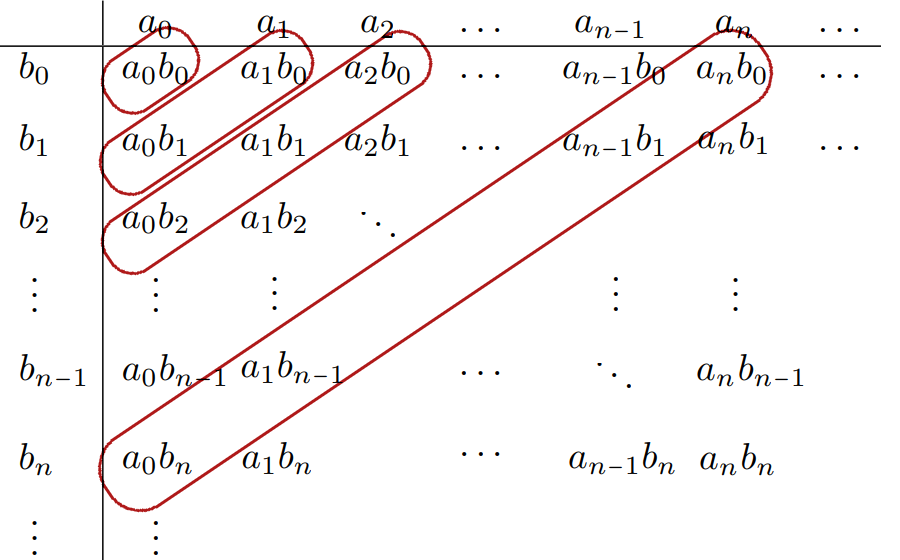
\includegraphics[width=0.4\textwidth]{tu/级数乘积.png}
    % \caption*{\texttt{各种分割的取样和,随着分割越来越细,趋于同一个数。}}
\end{wrapfigure}

直观上,如果我们把部分和序列的乘积的每一项纵横排列成表,那么上面的变换就是按斜对角线来将这些项加总。

我们希望求出表中所有项的和。但如果从横向和纵向来看,求每行、每列的和,都需要加无穷个数。
也就是说,要处理无穷次“无穷个数相加”。

如果每次先按斜对角线加总,再将这些和加总,那么只需要处理一次“无穷个数相加”。

因此,我们考虑通项为如下定义的级数:
$$ c_n = \sum_{i=0}^n a_i b_{n-i} . $$
如果级数$\sum a_n$、$\sum b_n$绝对收敛,记它们绝对值的级数和为$A^*$、$B^*$。
记级数$\sum c_n$的部分和序列为$\{C_n\}$,我们希望证明它趋于$AB$。

考察上图,前$n$个斜对角线的和加总,也可以看作$n$个纵列的和加总,因此:
$$C_n = \sum_{i=0}^{n} a_{n-i} B_i. $$
每项减去$a_{n-i}B$,再在最后一起加上,得到:
$$ C_n = \sum_{i=0}^{n} a_{n-i} (B_i - B) + \sum_{i=0}^n a_{n-i} B = \sum_{i=0}^{n} a_{n-i} (B_i - B) + A_n B. $$
因此,$C_n$和$AB$的差可以写为:
$$ |C_n - AB| = \left|\sum_{i=0}^{n} a_{n-i} (B_i - B) + (A_n - A) B \right|. $$
我们希望证明这个差趋于$0$。

随着$n$不断增大,$A_n$趋于$A$。因此关键在前面的求和项。其中$a_{n-i}$和$B_i - B$仿佛是“跷跷板”的关系。
$i$很大的时候,$B_i - B$足够小,而$i$很小的时候,$n-i$足够大,因此$a_{n-i}$又足够小。
因此,我们可以通过找特定的值将这些项分为两段,每段中的项$a_{n-i} (B_i - B)$都因为其中一个乘数足够小而足够小。

对任意$r>0$,首先由于$\{B_n\}$趋于$B$,因此可以找到$N$,使得$n\geqslant N$时总有:
$$ |B_n - B| \leqslant \frac{r}{3A^*}. $$

其次,对于$n<N$的情形,设$R$为$|B_n-B|$中最大的值,由于$\{a_n\}$趋于$0$,因此可以找到$M$,使得$n\geqslant M$时
总有:
$$ |a_n| \leqslant \frac{r}{3NR}.$$

最后,$A_n$趋于$A$,因此可以找到$L$,使得$n\geqslant L$时总有:
$$ |A_n - A| \leqslant \frac{r}{3|B|}.$$

于是,$n\geqslant L+M+N$时,
\begin{align*}
    |C_n - AB| &= \left|\sum_{i=0}^{n} a_{n-i} (B_i - B) + (A_n - A) B \right| \\
    &\leqslant  \sum_{i=0}^{n} |a_{n-i} ||B_i - B | + |A_n - A| |B|. 
\end{align*}
上式右边第一项可以在下标$N$处截成两段:
$$ \sum_{i=0}^{n} |a_{n-i} ||B_i - B | = \sum_{i=0}^{N-1} |a_{n-i}| |B_i - B| + \sum_{i=N}^{n} |a_{n-i}| |B_i - B| + |A_n - A| |B|,$$
$i<N$时,下标$n-i > n-N >M$,所以$|a_{n-i}| \leqslant \frac{r}{3NR}$,于是:
\begin{align*}
    |C_n - AB| &\leqslant \frac{r}{3NR} \sum_{i=0}^{N-1} |B_i - B| + \frac{r}{3A^*} \sum_{i=N}^{n} |a_{n-i}| + \frac{r}{3} \\
    &\leqslant \frac{r}{3NR} \cdot nR +  \frac{r}{3A^*} \sum_{i=0}^{+\infty} |a_i| + \frac{r}{3} \\
    &= \frac{r}{3} + \frac{r}{3A^*}\cdot A^* + \frac{r}{3} \\
    &= r.
\end{align*}
这就说明$\{C_n\}$趋于$AB$,级数$\sum c_n$收敛到$\sum a_n$、$\sum b_n$的级数和的乘积。
因此我们称$\sum c_n$是$\sum a_n$、$\sum b_n$乘积。

要注意的是,上面证明中没有用到$\sum b_n$绝对收敛的性质。实际上,只要$\sum a_n$、$\sum b_n$中有一个级数绝对收敛,
就可以定义乘积$\sum c_n$。如果两者都绝对收敛,那么$\sum c_n$也绝对收敛。

% 最后来看级数的除法。除法是乘法的逆运算,因此我们需要考察使得:
% $$ \forall n\in\mathbb{N} , \,\,\, a_n = \sum_{i=0}^n c_i b_{n-i} $$
% 的数列$\{c_n\}$。对于$n=0$,$a_0 = b_0 c_0$。如果$b_0 \neq 0$,那么
% $$ c_0 = \frac{a_0}{b_0} $$
% 满足条件。如果$b_0 = 0$,那么$c_0$不存在。

% 一般来说,如果$c_0, c_1, \cdots, c_{n-1}$已经求出,且$b_0\neq 0$,那么:
% $$ c_n = \frac{a_n - \sum_{i=0}^{n-1} c_i b_{n-i}}{b_0}$$
% 也就是说,只要$b_0\neq 0$,就可以按以上方法定义级数$\sum c_n$。

% 按照前面的方法,可以写出:
% $$A_n = \sum_{i=0}^{n} c_{n-i} B_i = \sum_{i=0}^{n} c_{n-i} (B_i - B) + C_n B $$
% 如果$B \neq 0$,那么由于$\{B_n\}$趋于$B$,可以找到$N$,使得$n\geqslant N$时总有
% $B_n > \frac{|B|}{2}$或总有$B_n < -\frac{|B|}{2}$。不妨设前者成立,那么:
% $$ \sum_{i=0}^{n} c_{n-i} B_i > \sum_{i=N}^{n} c_{n-i} \frac{|B|}{2} + \sum_{i=0}^{N-1} c_{n-i} B_i$$

% $$A_n = \sum_{i=0}^{n} b_{n-i} C_i = \sum_{i=0}^{N} b_{n-i} (C_i - C) + \sum_{i=N+1}^{n} b_{n-i} (C_i - C) + B_n C $$
% $$ \sum_{i=n-N}^{n} b_{i} (C_{n-i} - C) + \sum_{i=0}^{n-N-1} b_{i} (C_{n-i} - C) $$

% $$ a_n = 2^{-n}, b_0 = 1, b_n = -2^{-n}, n > 0 $$

% $$ c_0 = \frac{a_0}{b_0} = \frac{1}{1} = 1. $$
% $$ c_1 = \frac{a_1 - c_0b_1}{b_0} = \frac{0.5 - 1\cdot (-0.5)}{1} = 1. $$
% $$ c_2 = \frac{a_2 - c_0b_2 - c_1b_1}{b_0} = \frac{0.25 - 1\cdot (-0.25) - 1\cdot (-0.5)}{1} = 1. $$
% $$ c_n = \frac{a_n - c_0b_n - \cdots c_{n-1}b_1}{b_0} = \frac{2^{-n} + \sum_{i=1}^n 2^{-i}}{1} = 1. $$

\begin{sk}
    \mbox{} \\
    \indent 1. 为什么要用以上的方法定义收敛级数的乘积?你还能想到什么别的定义方式?和以上的定义相比,有哪些好处?有哪些坏处?\\
    \indent 2. 能否定义收敛级数的除法?
\end{sk}

\begin{xt}
    \mbox{} \\
    \indent 1. 设两级数$\sum a_n$、$\sum b_n$的通项分别是:
    $$ \forall n\in\mathbb{N}, \,\,\, a_n = \frac{(-1)^n}{\sqrt{n+1}}, \quad b_n = \frac{(-1)^n}{\sqrt{n+\frac{1}{2}}}. $$
    \indent 1.1. 证明:级数$\sum a_n$、$\sum b_n$收敛。\\
    \indent 1.2. 设级数$\sum c_n$的通项为:
    $$ c_n = \sum_{i=0}^n a_i b_{n-i} . $$
    \indent 证明:$|c_n| \geqslant 1$。\\
    % \begin{align*}
    %     |c_n| &= \left|\sum_{i=0}^n a_i b_{n-i}\right| \\
    %     &= \left|\sum_{i=0}^n \frac{1}{\sqrt{(i+1)(n-i+\frac{1}{2})}}\right| \\
    %     &\geqslant \left|\sum_{i=0}^n \frac{1}{\sqrt{\left(\frac{i+1+n-i+\frac{1}{2}}{2}\right)^2}}\right| \\
    %     &= \left|\sum_{i=0}^n \frac{2}{n+\frac{3}{2}}\right| \\
    %     &= \frac{2(n+1)}{n+\frac{3}{2}} \\
    %     &> 1.
    % \end{align*}
    \indent 1.3. 从以上两问的结果,你能得到什么结论?\\
    \indent 2. 设两级数$\sum a_n$、$\sum b_n$都绝对收敛。\\
    \indent 2.1. 考虑它们的乘积级数$\sum c_n$。证明:
    $$ \forall N, \,\,\, \sum_{n=0}^{N} |c_n| \leqslant \left(\sum_{n=0}^{+\infty} |a_n| \right) \cdot \left(\sum_{n=0}^{+\infty} |b_n| \right)$$
    % \begin{align*}
    %     \sum_{n=0}^{N} |c_n| &= \sum_{n=0}^{N} \left| \sum_{i=0}^n a_i b_{n-i} \right| \leqslant \sum_{n=0}^{N} \sum_{i=0}^n |a_i| |b_{n-i}| \\
    %     &\leqslant \sum_{n=0}^{2N} \sum_{\substack{0\leqslant i,j \leqslant n \\ i+j=n}} |a_i| |b_j| = \left(\sum_{n=0}^{N} |a_n| \right) \cdot \left(\sum_{n=0}^{N} |b_n| \right) \\
    %     &\leqslant \left(\sum_{n=0}^{+\infty} |a_n| \right) \cdot \left(\sum_{n=0}^{+\infty} |b_n| \right)
    % \end{align*}
    \indent 2.2. 证明$\sum c_n$绝对收敛。
\end{xt}

\chapter{连续函数的和}

小学的学习中,我们定义了有限个数的和。通过定义级数,我们学习了无穷多个数的求和。
不过,正如我们所知,无穷也有可数与不可数之分。级数定义了可数多个数的求和。
那么,是否能对不可数多个数求和呢?

举例来说,实数集是不可数集合,实数区间中的点也是不可数集合。
给定定义在实数集或某个区间$I$上的实变函数$f$,它将集合中每个点映射到函数值$f(x)$。
那么,能否对这些函数值求和呢?

这个问题比可数多个数的求和更为复杂,但在实际生活与生产中经常出现。
比如,我们通常假设时间是连续变量,而评估各种物理作用的效果时,通常需要研究一段时间内作用的效果。
例如,物体受的力在一定时间内的累计效果,称为冲量。它是物体导致速度变化的因素。
设物体在$t$时刻受力为$F(t)$,那么,
一段时间$[t_1; t_2]$上的冲量就是函数$F(t)$在$[t_1; t_2]$的累积。

另一个例子是带电物体的电荷累计。我们假设物体表面每个点上的电荷是连续分布的,一点$P$上的电荷密度是$g(P)$。
那么,物体表面的总电荷就是表面所有点上电荷密度的累积。

因此,我们有必要定义函数在区间、平面区域乃至更复杂的形体上的求和。
良好的定义并不是显而易见的。为这类求和给出符合实际生产生活中的需要的定义,
是一门深奥的学问。在当前阶段,我们只给出简要的介绍,研究特定情形下的求和工具,不作更深入的探索。

\section{函数图像的面积}

首先来看一个物理学中的例子。设物体受到方向恒定,大小随时间$t$变化的力$F(t)$。
定义$F(t)$在一段时间内的累积效果为冲量$I$。如果设物体刚受力时的冲量$I(0) = 0$,那么有定律:
$$ I(t) - I(0) = m(v(t) - v(0)).$$
其中$v$是物体的在受力方向上的速率。为了计算速率的改变量,我们希望计算$I(t)$,也就是$F(t)$的“和”。

以时间为横轴,画出函数$F$的图像。如果$F$的大小也是恒定的,
那么可以发现,$F$在一段时间$[t_1; t_2]$内的“总和”就是$F \cdot (t_2 - t_1)$。
从图像来看,函数图像是水平的线段,$F(t)$的“和”就是函数图像与$x$轴之间的矩形的面积。

\begin{figure}[h] %this figure will be at the right
    \vspace{4pt}
    \centering
    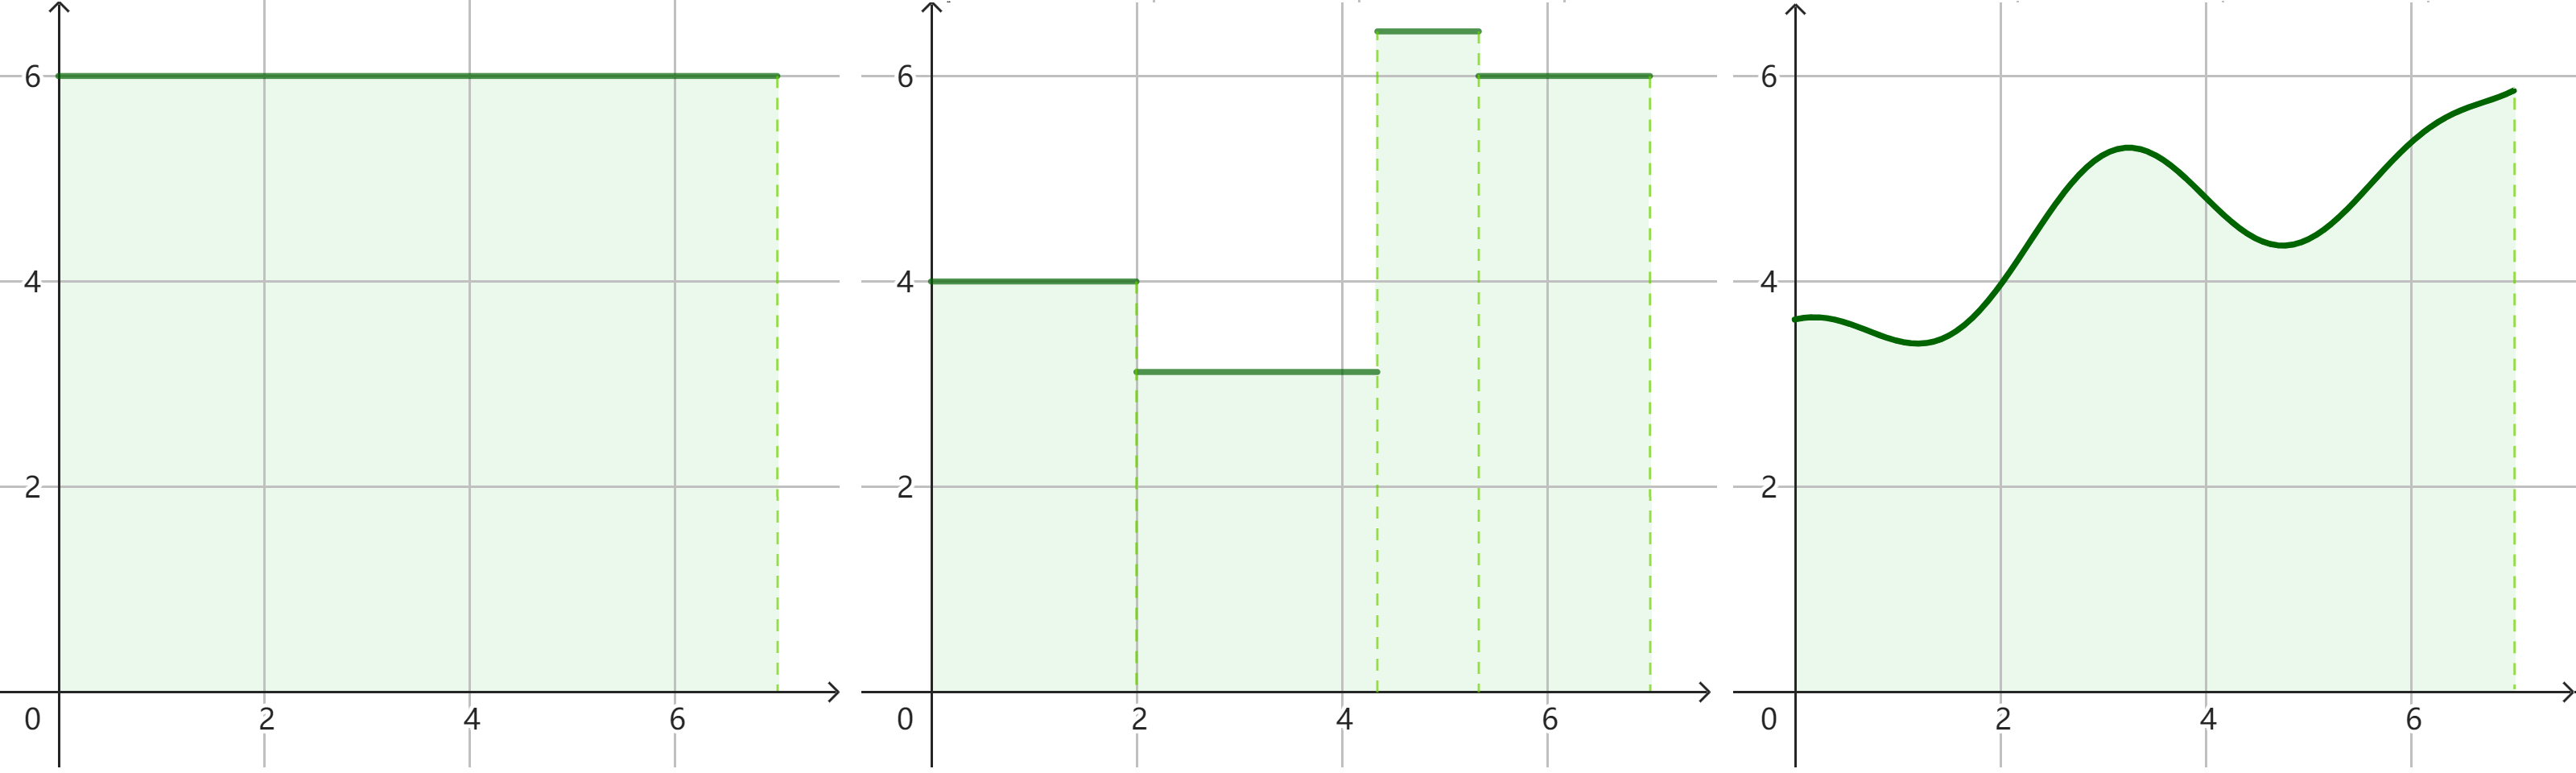
\includegraphics[width=\textwidth]{tu/积分定义1.png}
    \caption*{\texttt{函数图像与$x$轴之间的面积}}
\end{figure}

如果物体受力大小不恒定,但分段恒定,于是函数图像可以看作若干段水平线段。
于是,按分段求多个矩形的面积,然后求和,就得到$I$的改变量。

然而,更常见的情况是:$F$的大小随时间不断改变。这时候,我们如何求$F$的“和”呢?如何定义函数图像与$x$轴之间的面积?

需要知道的是,对一般的函数$F$,我们并不能很好地定义冲量$I$的改变量。不过,对于物理学中常见的模型
以及当前我们接触的简单形状来说,可以用比较简单的方法,定义“函数曲线与$x$轴之间的面积”。

提到面积,我们首先要回顾面积的基本性质。

\begin{po}
    边长为一的正方形,面积为一。
\end{po}

\begin{po}
    图形的面积是其各部分面积之和。
\end{po}

\begin{po}
    图形平移、旋转后,面积不变。对称的图形,面积相等。
\end{po}

\begin{po}
    相似形面积之比是相似比的平方。
\end{po}

根据以上的性质,
设有连续函数$f$,对于其定义域中的闭区间$[a; b]$,定义它在区间上的“面积”为$\int_a^b f$,称为它在闭区间$[a; b]$上的\textbf{积合}。
它可以看作连续函数区间上的不可数个值的“和”。如果$f$在某区间上可以定义积合,就说它在该区间上\textbf{可积}。

作为“面积”,我们对函数的积合有如下的基本要求:

\begin{enumerate}
    \item 函数$x\mapsto 1$在$[0;1]$上的积合是$1$。
    \item 设$a$、$b$、$c$是数轴上的三点,则
        $$\int_a^b f + \int_b^c f = \int_a^c f.$$
    \item 设$f$、$g$在$[a; b]$上可积,则
        $$ \int_a^b f + \int_a^b g = \int_a^b (f + g). $$
    \item 函数$x\mapsto f(x-c)$在$[a+c;b+c]$上的积合,等于$\int_a^b f$。
    \item 函数$x\mapsto f\left(\frac{x}{c}\right)$在$[ac; bc]$上的积合,等于$c\int_a^b f$。
    \item 函数$x\mapsto cf(x)$在$[a; b]$上的积合,等于$c\int_a^b f$。
    \item 如果$f$在区间上的值总介于$m$、$M$之间,那么
        $$m(b - a) \leqslant \int_a^b f \leqslant M(b - a).$$
\end{enumerate}
前六条分别对应四条公理。最后一条提出积合的基本大小关系。

要注意的是,这样定义的积合,作为“面积”,是有正负的。第二条中,令$a=b$,就有$\int_a^a f = 0$。
而令$a = c$,就有
$$\int_a^b f = - \int_b^a f.$$
第三条中,令$g=0$,就得到零函数的积合总是$0$。而令$g = -f$,就有
$$\int_a^b (-f) = -\int_a^b f. $$

从积合的基本性质可以推出一些常用的性质。比如:

\begin{tm}
    如果连续函数$f$在区间$[a; b]$上总大于等于$0$,那么它在区间上的积合也大于等于$0$。
\end{tm}

这个结论可以从积合的基本大小关系推出,而从此又能推出:

\begin{tm}
    如果连续函数$f$在区间$[a; b]$上总大于等于连续函数$g$,那么$f$在区间上的积合也大于等于$g$的积合。
\end{tm}

作为这个结论的特殊情况:

\begin{tm}
    考虑连续函数$f$的绝对值函数$|f|: x\mapsto |f(x)|$,则:
    $$ \left| \int_a^b f \right| \leqslant \int_a^b |f|. $$

\end{tm}

积合不仅定义了函数曲线的面积,也定义了区间的长度。只要令函数$f$为常函数$x\mapsto 1$,
那么$f$在区间上的积合就是区间的长度。换句话说,面积和长度,都是不可数个数在适宜定义下的和。

\begin{sk}
    \mbox{} \\
    \indent 1. 积合定义的区间长度和面积,与已有的定义是否相容?为什么这么说?\\
    \indent 2. 如何理解积合的正负?它与向量面积的正负相比有何异同?\\
    \indent 3. 除了区间,实数集的其他子集能否定义长度?你能想到为哪些集合定义长度?和区间的长度是否相容?\\
    \indent 4. 本节定义的积合是否一定存在?为什么?
\end{sk}

\begin{xt}
    \mbox{} \\
    \indent 1. 设有集合$S$,$S$的元素是不小于零的实数。$S$中所有数的和是有限的实数$w$。\\
    \indent 1.1. 对正整数$n$,考虑$S$的子集$S_n$:$S_n = \{x\in S \, | \, x \geqslant \frac{1}{n}\}$。证明:$S_n$总是有限集合。\\
    \indent 1.2. 证明:$S$的元素中,至多有可数个元素大于$0$。\\
    \indent 2. 设函数$f$在闭区间$[a; b]$上连续且大于等于零,在区间中某一点处大于零。\\
    \indent 2.1. 证明:可以找到某个正数$r$和$[a; b]$的某个子区间$[c;d]$,使得$f$在$[c;d]$上总大于$r$。\\
    \indent 2.2. 证明:$f$在$[a; b]$上的积合大于零。\\
    \indent 3. 证明:$\int_0^1 (1 - x) = \int_0^1 x$。\\
    \indent 4. 设有函数$f: x\mapsto \frac{x}{x^2+1}$,求$\int_{-1}^1 f$。\\
\end{xt}

\section{积合与微变}
从积合的基本性质出发,还可以得到积合与微变的重要关系:

\begin{tm}{\textbf{微积互反定理}}
    \mbox{} \\
    1. $f$是闭区间$[a; b]$上的连续函数。考虑函数$G: x\mapsto \int_a^x f$,则$G$在$[a; b]$上可微,
    $G(a) = 0$,且
    $$\forall \,\, x\,\,\in(a; b), \,\,\, \partial G (x) = f(x).$$
    2. 设函数$f$在闭区间$[a; b]$上可微,且微变函数连续(称为\textbf{连续可微}),则:
    $$ \forall \,\, x\,\,\in(a; b), \,\,\, \int_a^x \partial f = f(x) - f(a) $$
\end{tm}

\begin{proof}
    1. 考虑$G$的变率。根据基本性质,对任意$x\in(a; b)$和$h>0$:
    $$ \frac{G(x+h) - G(x)}{h} = \frac{\int_a^{x+h} f - \int_a^x f}{h} = \frac{\int_x^{x+h} f}{h}. $$
    考虑闭区间$[x; x+h]$,$f$是连续函数,因此在区间上达到最大最小值。记$f$取得最大最小值的点为$\overline{x}$和$\underline{x}$,
    即
    $$ \forall t \in [x; x+h] ,\,\,\, f(\underline{x}) \leqslant f(t) \leqslant f(\overline{x}). $$
    于是根据基本性质,
    $$ h\cdot f(\underline{x}) \leqslant \int_x^{x+h} f \leqslant h\cdot f(\overline{x}). $$
    即
    $$ f(\underline{x}) \leqslant \frac{G(x+h) - G(x)}{h} = \frac{\int_x^{x+h} f}{h} \leqslant f(\overline{x}). $$
    $\underline{x}$、$\overline{x}$都在区间$[x; x+h]$中,而$f$是连续函数,因此,当$h$趋于$0$的时候,
    $f(\underline{x})$、$f(\overline{x})$都趋于$f(x)$。根据同归定理,变率$\frac{G(x+h) - G(x)}{h}$也趋于$f(x)$:
    $$ \lian{h\to 0} \frac{G(x+h) - G(x)}{h} = f(x).$$
    这说明$G$在$x$处可微,且微变率$\partial G (x) = f(x)$。

    2. 考虑$H: x\mapsto f(x) - \int_a^x \partial f$,它是可微函数,而且微变为:
    $$ \forall \,\, x\,\,\in(a; b), \,\,\, \partial H(x) = \partial f(x) - \partial f(x) = 0. $$
    因此$H$是常函数,设$H$的值为$c$,则
    $$f(x) = \int_a^x \partial f + c, $$
    令$x = a$,就有
    $$f(a) = 0 + c,$$
    即$c = f(a)$,所以
    $$ \forall \,\, x\,\,\in(a; b), \,\,\,\int_a^x \partial f = f(x) - f(a).$$

\end{proof}

微积互反定理说明,如果把积合看作对函数的运算,那么积合是微变运算的逆运算。
给定区间$[a; b]$上的连续函数$f$,必然有唯一的连续可微函数$G$,
使得$G(a) = 0$,且$\partial G = f$。给定$[a; b]$上的连续可微函数$f$,必然有唯一连续函数$\partial f$,
其积合是$f$。

我们说$\int_a^x f$是$f$的\textbf{积合函数},$f$是积合的\textbf{被积函数}。
已知被积函数,求积合函数,或某个区间上的积合,称为\textbf{求合}。

从上面的推导可知,积合函数加上常数,仍然是积合函数。

\begin{et}
    \mbox{} \\
    \indent 1. 对自然数$n$,求多项式函数$x\mapsto x^n$的积合函数。\\
    \indent 2. 对正数$a\neq 1$,求幂函数$x\mapsto a^x$的积合函数。\\
    \indent 3. 求正弦函数和余弦函数的积合函数。
\end{et}

\begin{so}
    \mbox{} \\
    \indent 1. 函数$H: x\mapsto \frac{x^{n+1}}{n+1}$的微变函数是$x\mapsto x^n$,所以根据微积互反定理,
    $H$是$x\mapsto x^n$的积合函数。\\
    \indent 2. 函数$H: x\mapsto \frac{a^x}{\ln{a}}$的微变函数是$x\mapsto a^x$,所以根据微积互反定理,
    $H$是$x\mapsto a^x$的积合函数。\\
    \indent 3. 正弦函数$\sin$的微变函数是余弦函数$\cos$,余弦函数$\cos$的微变函数是$-\sin$,
    所以$-\cos$是正弦函数的积合函数,$\sin$是余弦函数的积合函数。
\end{so}

我们研究过微变函数与函数的四则运算的关系。那么积合函数是否与四则运算兼容呢?

从基本性质可知,积合与函数的加减法兼容:
$$ \int_a^x (f \pm g) = \int_a^x f \pm \int_a^x g. $$

但是,积合与函数的乘法并不兼容。换句话说,下面的关系并不成立:
$$ \int_a^x (f \cdot g) = \int_a^x f \cdot \int_a^x g. $$

这是因为函数乘积的微变函数比较“不规则”:
$$ \partial (f\cdot g) = \partial f \cdot g + f \cdot \partial g.$$

因此,对两边分别求合,我们只能得出:
$$ f(x)\cdot g(x) - f(a)\cdot g(a) = \int_a^x \partial (f\cdot g) = \int_a^x (\partial f \cdot g) + \int_a^x (f \cdot \partial g). $$

由于积合与乘法不兼容,我们无法像微变一样方便地求出很多经典函数的积合函数。
反而一些表达式“不太规则”的函数,因为是某些函数的微变函数,所以根据微积互反定理,能求出积合函数。
如果某个函数的积合函数可以用经典函数表示,就说它\textbf{显式可积};否者说它\textbf{显式不可积}\footnote{常见的显式可积函数,及它们的积分,参见附录$C$的“常见积分表”。}。

函数显式不可积,不表示它不可积。
比如,函数$x\mapsto \frac{e^x}{x}$的积合函数无法用经典函数表示出来,它是显式不可积的函数。
但它在区间$[1;2]$上连续,因此可积。
给定$a>1$,我们可以肯定$x\mapsto \frac{e^x}{x}$在$[1; a]$上的积合存在,是某个大于$0$的数,
但我们无法简单用有理式、幂函数、三角函数这些经典函数算出它的值。

为了方便地求函数的积合,我们希望能找出更多显式可积的函数。
为此,数学家发展了一些求合的转化技巧,把看起来显式不可积的被积函数转化为显式可积的函数。

从函数乘法的积合出发,我们考虑这样的特殊情形:
求两个连续函数$f$、$g$的乘积的积合,如果其中一个(比如$g$)连续可微,那么
$$ \int_a^x (f \cdot g) = F(x)\cdot g(x) - F(a)\cdot g(a) - \int_a^x (F \cdot \partial g). $$
其中$F$是$f$的积分函数。

通过这个关系,我们可以把乘积$fg$的积合转化为$F\partial g$的积合。这个转化技巧称为\textbf{分部积合法}。
使用分部积合法,可以把一些看起来显式不可积的函数转为显式可积的函数。

\begin{et}
    \mbox{} \\
    \indent 1. 使用分部积合法,求函数$x\mapsto x \sin{x}$的积合函数。\\
    \indent 2. 使用分部积合法,求函数$x\mapsto e^x \sin{x}$的积合函数。\\
\end{et}

\begin{so}    
    \mbox{} \\
    \indent 1. 考虑函数$F(x) = -\cos{x}$,则$\partial F = \sin{x}$,因此,
    \begin{align*}
        \int_a^x (x\sin{x}) &= \int_a^x (\sin{x}\cdot x) = \int_a^x (\partial F(x) \cdot x) \\
        &= F(x)\cdot x - F(a)\cdot a - \int_a^x (F(x) \cdot \partial x) \\
        &= -x\cos{x} + a\cos(a) + \int_a^x (\cos{x} \cdot 1) \\
        &= -x\cos{x} + a\cos(a) + \int_a^x \cos{x} \\
        &= -x\cos{x} + a\cos(a) + \sin{x} - \sin{a}.
    \end{align*}
    \indent 2. 考虑函数$F(x) = e^x$,它的微变函数是自己。因此,
    \begin{align*}
        \int_a^x \left(e^{x} \sin{x}\right) &= \int_a^x \left(e^x\cdot \sin{x}\right) = \int_a^x \left(\partial F(x) \cdot \sin{x}\right) \\
        &= F(x)\sin{x} - F(a)\sin(a) - \int_a^x \left(e^{x} \cdot \partial \sin{x}\right) \\
        &= e^x\sin{x} - e^a\sin(a) - \int_a^x \left(e^x \cos{x}\right) .
    \end{align*}
    用同样的方法,可以求出
    $$  \int_a^x \left(e^x \cos{x}\right) = e^x\cos{x} - e^a\cos(a) + \int_a^x \left(e^{x} \sin{x}\right). $$
    代入前面的关系式,得到:
    $$ \int_a^x \left(e^{x} \sin{x}\right) = e^x\sin{x} - e^a\sin(a) - e^x\cos{x} + e^a\cos(a) - \int_a^x \left(e^{x} \sin{x}\right). $$
    因此
    $$ \int_a^x \left(e^{x} \sin{x}\right) = \frac{1}{2}\big(e^x(\sin{x} - \cos{x}) - e^a(\sin(a) - \cos(a))\big).$$
\end{so}

最后考虑函数的复合与积合。设连续函数$f$在区间$[a; b]$上连续,而函数$g$在区间$[f(a), f(b)]$上连续。
复合函数$g\circ f$的微变为:
$$ \partial (g \circ f) (x) = \partial g(f(x)) \partial f (x). $$

因此,如果设$G$是$g$的积分函数,那么
$$ \partial (G \circ f) (x) = g(f(x)) \partial f (x). $$
两边积合,就得到:
$$ G(f(x)) - G(f(a)) = \int_a^x \left( g(f(x)) \partial f (x) \right).$$
而左边可以看作$g$在$[f(a), f(b)]$上的积合。也就是说:
$$ \int_a^x \left( g(f(t)) \partial f (t) \right) = \int_{f(a)}^{f(x)} g.$$

从这个关系式出发,可以得到另一种积合转化技巧。如果某个被积函数能写成$g(f(t)) \partial f (t)$的形式,
那么可以将它的积合转为$g$关于$u = f(t)$的积合。反之,如果将被积函数$g$的自变量$x$看作函数$x = f(u)$,那么
积合就变成$g(f(u)) \partial f (u)$的形式。这个方法也称为\textbf{换元积合法}。

\begin{et}
    \mbox{} \\
    \indent 1. 使用换元积合法求$\int_0^2 \frac{x}{x^2 + 1}$。 \\
    \indent 2. 使用换元积合法求$\int_0^2 \frac{1}{\sqrt{x} + 1}$。
\end{et}

\begin{so}
    \mbox{} \\
    \indent 1. 考虑$g: x\mapsto \frac{1}{x + 1}$和$f: x\mapsto x^2$,则
    $$ \int_0^2 \left( g(f(x)) \partial f (x) \right) = \int_0^2 \frac{2x}{x^2 + 1}. $$
    因此,
    \begin{align*}
        \int_0^2 \frac{x}{x^2 + 1} &= \frac{1}{2} \int_0^2 \left( g(f(x)) \partial f (x) \right) \\
        &= \frac{1}{2}\int_{f(0)}^{f(2)} g = \frac{1}{2}\int_0^4 \frac{1}{x + 1} 
    \end{align*}
    函数$x\mapsto \ln{(x + 1)}$的微变是$g$,因此,
    \begin{align*}
        \int_0^2 \frac{x}{x^2 + 1} &= \frac{1}{2}\int_0^4 \frac{1}{x + 1} \\
        &= \frac{1}{2}\left(\ln{(4 + 1)} - \ln{(0 + 1)}\right) = \frac{\ln{5}}{2}.
    \end{align*}

    \indent 2. 记被积函数为$g$。考虑$f: x\mapsto x^2$。$x$从$0$运动到$\sqrt{2}$时,$f(x)$从$0$运动到$2$。因此:
    \begin{align*}
        \int_0^2 \frac{1}{\sqrt{x} + 1} &= \int_{f(0)}^{f(\sqrt{2})} g \\
        &= \int_0^{\sqrt{2}} \left( g(f(x)) \partial f (x) \right) \\
        &= \int_0^{\sqrt{2}} \frac{2x}{x + 1} = 2\int_0^{\sqrt{2}} \left( 1 - \frac{1}{x + 1} \right) \\
        &= 2\int_0^{\sqrt{2}} 1 - 2\int_0^{\sqrt{2}} \frac{1}{x + 1} \\
        &= 2(\sqrt{2} - 0) - 2 \left(\ln{(\sqrt{2} + 1)} - \ln{(0 + 1)}\right) \\
        &= 2\sqrt{2} - 2\ln{(\sqrt{2} + 1)}.
    \end{align*}
\end{so}

\begin{sk}
    \mbox{} \\
    \indent 1. 函数的积合函数与一次函数有什么共同点? \\
    \indent 2. 函数的商的积合函数有什么规律?\\
    \indent 3. 反函数的积合函数有什么规律?\\
    \indent 4. 如果函数的积合函数无法用经典函数表示,如何计算它的积合?你有什么想法?\\
    \indent 5. 如何计算以下函数的微变?
    $$x\mapsto \int_0^{f(x)} g.$$
\end{sk}

\begin{xt}
    \mbox{} \\
    \indent 1. 求以下函数的积合函数。\\
    \indent 1.1. $x\mapsto 3x^2 + 1 - x$。\\
    \indent 1.2. $x\mapsto \frac{1}{x}$。\\
    \indent 1.3. $x\mapsto \ln{x}$。\\
    \indent 1.4. $x\mapsto \frac{1}{x^2 + 1}$。\\
    \indent 2. 使用分部积合法求以下函数的积合。\\
    \indent 2.1. $x\mapsto x^2 \cos{x}$。 \\
    \indent 2.2. $x\mapsto x \ln{x} $。 \\
    \indent 2.3. $x\mapsto e^x \cos{x} $。 \\
    \indent 3. 使用换元积合法求以下函数的积合。\\
    \indent 3.1. $x\mapsto \sin^2{x} \cos{x}$。 \\
    \indent 3.2. $x\mapsto \frac{\ln{x}}{x} $。 \\
    \indent 3.3. $x\mapsto \tan{x} $。 \\
    \indent 4. 对正整数$n\geqslant 2$,设$I_n = \int_1^2 \left(x^{-n}e^{\frac{1}{x}}\right)$。\\
    \indent 4.1. 计算$I_2$。\\
    \indent 4.2. 使用分部积合法,证明:
            $$ I_{n+1} = e - \frac{\sqrt{e}}{2^{n-1}} + (1 - n)I_n.$$
    \indent 4.3. 计算$I_3$。\\
    \indent 4.4. 证明:$x>1$时,$0\leqslant x^{-n}e^{\frac{1}{x}} \leqslant \frac{e}{x^n}$。\\
    \indent 4.5. 根据上一问的结论,给出$I_n$的范围,并求数列$\{I_n\}_{n\in\mathbb{N}}$的极限。
\end{xt}

\section{积合与函数}

和微变一样,积合也可以作为研究函数的工具。比如,从微变中值定理出发,可以得到积合的中值定理\footnote{证明见附录$C$。}。

\begin{tm}{\textbf{积合中值定理}}
    如果函数$f$在闭区间$[a; b]$上连续,那么可以找到$c\in[a;b]$使得:
    $$ \int_a^b f = (b - a)\cdot f(c).$$
\end{tm}

直观上,可以这样理解:把$f$在闭区间$[a; b]$上的积合看作函数到$x$轴的面积,
那么它介于分别以$f$在$[a; b]$上的最小值、最大值为高的矩形的面积之间。

想象我们有一个长方的水箱,侧面从左到右画了函数的曲线。水位一开始处于曲线最低处。
不断加水让水位升高,直到水位和曲线最高处平齐。水位以下的面积和曲线下的面积相比,从一开始前者小于后者,连续变化,
到最后前者大于后者。因此,水位上涨过程中总有一刻,水位以下的面积等于曲线下的面积。
这时水位线和曲线的交点,就是我们要找的$f(c)$。

\begin{figure}[h] %this figure will be at the right
    \vspace{4pt}
    \centering
    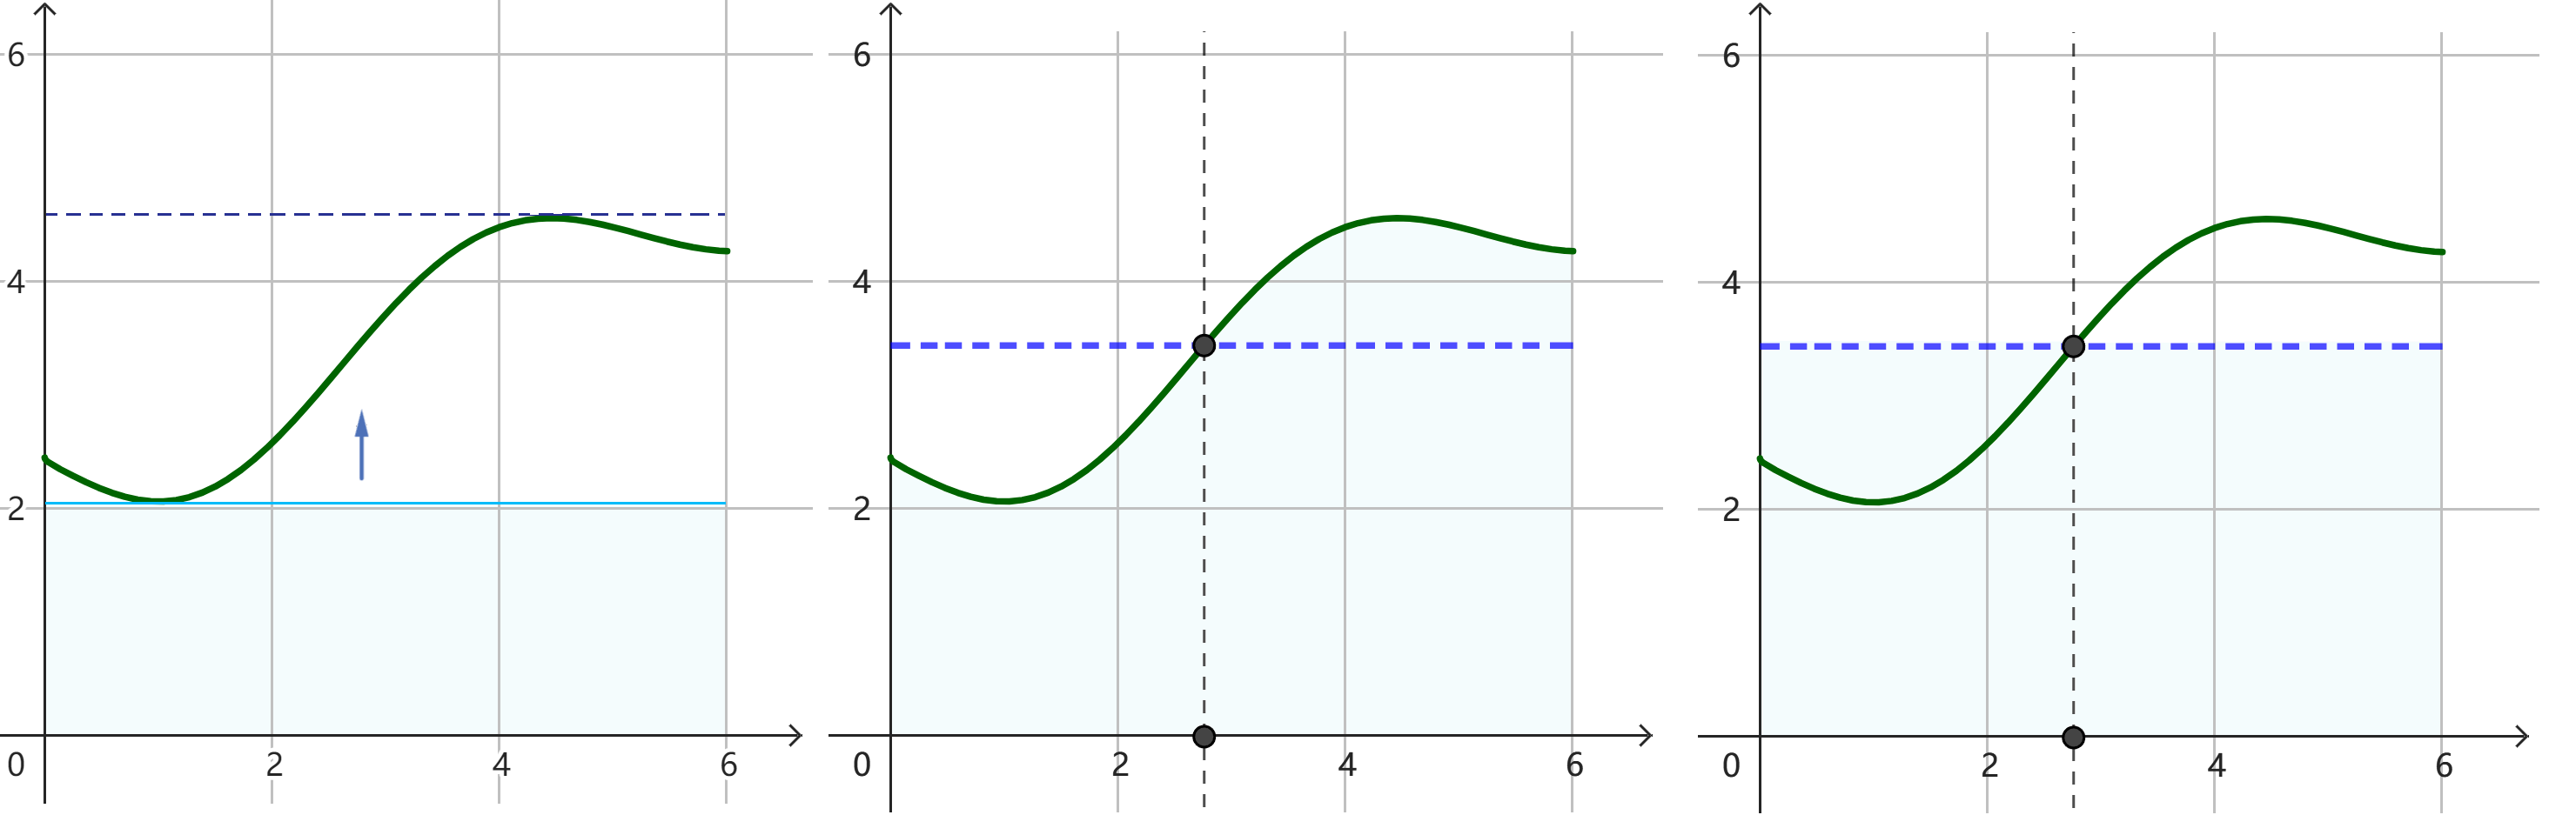
\includegraphics[width=\textwidth]{tu/积分中值定理1.png}
    \caption*{\texttt{如左图,水位从曲线最低的位置开始上涨,当水位下的面积等于曲线下的面积时,水位线与曲线的交点就是}$c$\texttt{的位置。}}
\end{figure}

如果函数$f$连续可微,从微积互反定理可以得到:
$$ f(b) = f(a) + \int_a^b \partial f .$$
因此,$f$在一点$a$附近的值,可以通过加上微变的积分得到。从这个思想出发,可以得到另一种局部展开函数的方法。

\begin{tm}{\textbf{积合余项的微变展开定理}}
如果函数$f$在包含实数$a$的区间$I$中$n+1$次可微,且$n+1$次微变函数连续,那么对$I$中另一点$x$有:
\begin{align*}
    f(x) &= f(a) + \sum_{i=1}^n \frac{\partial^i f(a)}{i!} (x - a)^i + \int_a^x \frac{(x - t)^{n}}{n!} \partial^{n+1} f(t)\mathrm{d}t. \\
    &= P_n + Y_n 
\end{align*}
其中$Y_n = \int_a^x \frac{(x - t)^{n}}{n!} \partial^{n+1} f(t)\mathrm{d}t$称为局部展开的$n$次积合余项\footnote{如果被积函数的表达式里有不止一个变量,为了区别,我们一般会在被积函数后面加上符号$\mathrm{d}$和要求积合的变量,指明我们在对哪个变量求积合。比如这里我们加上了$\mathrm{d}{\color{red}t}$,表示对变量$t$求积合,而不是$a$和$x$。}。

\end{tm}

这个定理和微变展开定理很相似,都是把$a$附近的函数值用$a$处的函数值和微变率组成的多项式$P_n$表示。
两者的不同主要在于对函数可微程度的要求以及余项的形式。

我们把之前微变展开定理的余项称为\textbf{微变余项}。
$$
\begin{array}{lll}
    \mbox{{\bfseries 微变余项}} & \phantom{1}\qquad\qquad\qquad & \mbox{{\bfseries 积合余项}} \\
    & \\
    \displaystyle \frac{\partial^{n+1} f (c)}{(n+1)!}(x - a)^{n+1} & \phantom{1}\qquad\qquad\qquad & \displaystyle \int_a^x \frac{(x - t)^{n}}{n!} \partial^{n+1} f(t)\mathrm{d}t \\
\end{array}
$$
微变余项只要求函数在$a$附近$n+1$次可微,
只和$n+1$次微变函数在某点的值有关,但无法给出该点的确切位置。
积合余项不需要引入不知位置的点,但要求$n+1$次微变函数连续。

\begin{sk}
    \mbox{} \\
    \indent 1. 比较微变中值定理和积合中值定理,说说两者的区别和联系。\\
    \indent 2. 比较两个微变展开定理的余项形式,说说两者的区别和联系。
\end{sk}

\begin{xt}
    \mbox{} \\
    \indent 1. 设函数$f$和$g$在闭区间$[a; b]$上连续,证明:可以找到$c\in[a; b]$,使得:
    $$ \int_a^b (f\cdot g) = f(c) \cdot \int_a^b g.$$
    \indent 2. 设有定义在$\mathbb{R}$上的周期函数$f$,周期为$T>0$,证明:
    $$ \forall \,\, a \in \mathbb{R},\,\,\, \int_a^{a+T} f = \int_0^{T} f .$$
    \indent 3. 考虑函数$f:x \mapsto \ln{\left(1+x^2\right)}$。\\
    \indent 3.1. 求$\partial f$、$\partial^2 f$,将$f$在$0$处展开到$2$次。\\
    \indent 3.2. 证明:
    $$ \int_0^1 \frac{(1-t)^2(1+t)}{\left(1+x^2\right)^2} = \frac{\ln{2}}{2}.$$
\end{xt}

\begin{appendix}

\chapter{无穷集合的势}

\begin{df}{\textbf{像和原像}}\label{df:a-1-0}
    给定映射$f$,记$f$的定义域为$D$。
    $f$将集合$A\subseteq D$映射得到的集合,称为$A$经过$f$映射的\textbf{像},记作$f(A)$。
    给定$f$值域的子集$B$,将集合:
    $$ \{x \in D \, | \, f(x) \in B \}$$
    称为$B$(关于$f$)的\textbf{原像}。
\end{df}

\begin{po}{\textbf{选择公理}}
    可以同时从任意多个非空集合里各选择一个元素,构成一个新集合。
\end{po}

从选择公理出发,我们可以得出一些有用的基本结论。

\begin{tm}{\textbf{构造双射}}\label{tm:a-1-0}
    设$f$是从集合$A$到$B$的单射,那么$f$是$A$到$f(A)$的双射。

    设$f$是从集合$A$到$B$的满射,那么存在从$A$的子集到$B$的双射$g$,使得$g(x) = f(x)$总成立。
\end{tm}

这个定理其实说明了单射和满射相比双射“缺了什么”,以及如何修正,得到双射。

单射的“问题”在于它的值域“填不满”到达域,构不成满射。因此,把到达域中不在它值域里的部分去掉,
只考虑它的值域作为到达域,那么它就是双射了。

满射的“问题”在于应变量可能是多个自变量映射的结果,也就是“多对一”,导致不是单射。
因此,只要在里面选一个自变量就好了。而选择公理告诉我们,这么做是没问题的。

\begin{proof}
    首先证明,可以从单射构造双射。设$f$是从集合$A$到$B$的单射,那么按照定义,
    $f$是$A$到$f(A)\subseteq B$的满射。

    $f$既是单射又是满射,因此$f$是$A$到$f(A)$的双射。

    再证明可以从满射构造双射。设$f$是从集合$A$到$B$的满射,那么按照定义,
    $B$中每个元素$y$关于$f$的原像都是非空集合。

    考虑$B$所有元素关于$f$的原像。根据选择公理,可以同时在这些原像中各选择一个元素。
    这样构成的集合是$A$的子集$A'$。

    我们定义新的映射
    \begin{align*}
        g: A' &\rightarrow B \\
        x &\mapsto f(x)
    \end{align*}
    
    这样定义的$g$,是从$A$的子集$A'$到$B$的满射。而且按照定义,总有$g(x) = f(x)$。
    而由于不同的自变量$x$来自不同的原像,所以经过$f$映射的结果也不相同。这说明$g$是单射。因此$g$是双射。

\end{proof}

\begin{df}{\textbf{集合上的序}}
    给定一个集合,可以对其中的元素指定顺序。具体来说,序是一种二元关系。
    比如,整数集、有理数集或实数集上的大于、小于、大于等于、小于等于关系,都是序关系。

    如果序关系$\triangleleft$满足以下条件,就称为\textbf{偏序}:
    \begin{enumerate}
        \item 自返性:$\forall x, \,\,\, x \triangleleft x$。
        \item 反称性:$\forall x, y$,如果$x \triangleleft y$且$y \triangleleft x$, 那么$x = y$。
        \item 传递性:$\forall x, y, z$,如果$x \triangleleft y$且$y \triangleleft z$, 那么$x \triangleleft z$。
    \end{enumerate}
    配备有偏序关系的集合称为\textbf{偏序集}。

    偏序集不保证集合中任意两个元素都有序关系。如果集合中任意两个元素$x, y$,总有$x \triangleleft y$或$y \triangleleft x$成立,
    就说序关系是\textbf{全序},集合是\textbf{全序集}。

    给定$S$上的序关系$\triangleleft$,如果集合$S$中有元素$x$,使得$x \triangleleft y$对$S$中任意元素$y$成立,
    就说$x$是$S$的\textbf{最小元}。如果集合$S$中有元素$x$,使得$y \triangleleft x$对$S$中任意元素$y$成立,
    就说$x$是$S$的\textbf{最大元}。比如,正整数集上的小于等于关系,就有最小元$1$,通常称为最小值。
    
    如果序关系使得集合的任意非空子集总有最小元,就说它是\textbf{良序},集合是\textbf{良序集}。
    比如,正整数集上的小于等于关系就是良序。

    % 给定集合$S$上的序关系$\triangleleft$,对$S$的元素$u$和子集$T$,如果$T$中任意元素$x$总有$x\triangleleft u$,
    % 就说$u$是$T$的\textbf{上界}。$T$的所有上界构成$S$的子集$T^{\text{上}}$。如果$T^{\text{上}}$有最小元,
    % 就说这个最小元是$T$的\textbf{上确界}或\textbf{最小上界}。

    % 设$S$上有偏序$\triangleleft$,$S$的子集$T$如果是全序集,就称为\textbf{序上的链}。
    % 如果$S$中的偏序$\triangleleft$上的任何链都有上确界,就说$S$在\textbf{序}$\triangleleft$\textbf{上闭合}。
\end{df}

% \begin{tm}{\textbf{最大值定理}}
%     设有集合$S$,$S$上有偏序$\triangleleft$。已知$S$的任何子集$T$如果是全序集,就有上确界。
%     那么,$S$有最大元。
% \end{tm}

\begin{df}\label{df:a-1-10}
    设有集合$A$和$B$。
    \begin{itemize}
        \item 如果存在$A$到$B$的双射,就说$A$和$B$的势相等,两者等势,记作$|A| = |B|$。
        \item 如果存在从$A$到$B$的单射,就说$A$的势不大于$B$的势或$A$的势小于等于$B$的势,记作$|A| \leqslant |B|$或$|B| \geqslant |A|$。
        \item 如果存在从$A$到$B$的单射,但不存在$B$到$A$的单射,就说$A$的势小于$B$的势,记作$|A| < |B|$或$|B| > |A|$。
    \end{itemize}
\end{df}

\begin{tm}{\textbf{等势定理}}\label{tm:a-1-10}
    给定集合$A$、$B$,如果$|A| \leqslant |B|$、$|B| \leqslant |A|$,那么$|A| = |B|$。
\end{tm}

这个定理是判定集合等势的重要方法。它的证明思路大致是这样的:
我们有从$A$到$B$的单射$f$,也有从$B$到$A$的单射$g$。
根据前面的结论,
$f$是$A$到$B$子集的双射,$g$又把$B$的这部分一一对应到$A$的一部分,于是变成“更小”的双射。
这个相互跳转的过程,集合$A$、$B$会不断“剥离出”一部分。
它们是通过双射得到的,所以它们之间可以建立双射。
而双方剩下的部分也可以建立双射。于是我们就在$A$、$B$之间建立了双射。

\begin{proof}
    根据条件,存在从$A$到$B$的单射$f$,以及从$B$到$A$的单射$g$。记以下集合:
    $$
    \begin{array}{rlrl}
        A_0&= A, \quad & B_0 &= B \\
        A_1&= g(B_0), \quad & B_1 &= f(A_0) \\
        A_2&= g(B_1), \quad & B_2 &= f(A_1) \\
        &\vdots & &\vdots \\
        A_{n+1}&= g(B_n), \quad & B_{n+1} &= f(A_n) \\
        &\vdots & &\vdots
    \end{array}
    $$
    根据定理\ref{tm:a-1-0},$f$是$A_0$到$B_1$的双射,$g$是$B_1$到$A_2$的双射,等等。
    因此,我们可以写出以下两条等势关系“链”:
    \begin{align*}
        |A| = |A_0| = |B_1| = |A_2| = |B_3| = |A_4| = |B_5| = |A_6| = \cdots  \\
        |B| = |B_0| = |A_1| = |B_2| = |A_3| = |B_4| = |A_5| = |B_6| = \cdots   
    \end{align*}
    其中集合的关系为:
    \begin{align*}
        A = A_0 \supseteq A_1 \supseteq A_2 \supseteq A_3  \supseteq \cdots  \\
        B = B_0 \supseteq B_1 \supseteq B_2 \supseteq B_3  \supseteq \cdots   
    \end{align*}
    
    以上集合关系中,如果对某个正整数$n$,有$A_n = A_{n+1}$或$B_n = B_{n+1}$,那么两条等势“链”就连上了,于是立刻得到$|A| = |B|$。

    如果所有的集合关系都是$A_n \subset A_{n+1}$、$B_n \subset B_{n+1}$,即真子集关系,
    那么考虑$A_n$中去掉$A_{n+1}$的部分,记为$A_n^*$。同理定义$B_n^*$。
    
    $A_n$到$B_{n+1}$有用$f$定义的双射,$A_{n+1}$到$B_{n+2}$有用$f$定义的双射,
    因此,$A_n^*$到$B_n^*$也有用$f$定义的双射。我们可以得到以下两条等势关系“链”:
    \begin{align*}
        |A_0^*| = |B_1^*| = |A_2^*| = |B_3^*| = |A_4^*| = \cdots  \\
        |B_0^*| = |A_1^*| = |B_2^*| = |A_3^*| = |B_4^*| = \cdots   
    \end{align*}
    $|A_0^*| = |B_1^*|$,$|A_1^*| = |B_0^*|$,而$A_0^*$与$A_1^*$不相交,
    而$B_0^*$与$B_1^*$不相交。
    因此,这两对集合可以拼成$A_0^* \cup A_1^*$到$B_0^* \cup B_1^*$的“整齐”的双射。
    其中$A_0^*$的元素映射到$B_1^*$,$B_0^*$的元素映射到$A_1^*$,互不干扰。
    
    对于一般的相邻奇偶数下标,
    也可以这么做。因此,我们可以构建这样的映射:
    \begin{align*}
        h : \bigcup_{n\in\mathbb{N}} A_n^* &\rightarrow \bigcup_{n\in\mathbb{N}} B_n^*  \\
        x \quad&\mapsto \left\{ \begin{array}{ll}
            f(x) & \mbox{如果} x\in A_{2m}^*,\,\,\, m\in\mathbb{N}  \\
            g(x) & \mbox{如果} x\in A_{2m+1}^*,\,\,\, m\in\mathbb{N} 
        \end{array} \right.
    \end{align*}
    由于对所有的$n$,$A_n^*$两两不相交,$B_n^*$两两不相交。所以以上定义的$h$成立,而且是双射。

    如果集合$A^* = \bigcup_{n\in\mathbb{N}} A_n^*$就是$A$,同理$B^* = \bigcup_{n\in\mathbb{N}} B_n^*$就是$B$,
    我们就在$A$和$B$之间建立了双射。不过很可惜,$A^*$还不是$A$,遗漏了一部分元素。

    遗漏了怎样的元素呢?按照定义,$\bigcup_{n\in\mathbb{N}} A_n^*$是所有“在某个$A_n$中但不在$A_{n+1}$中”
    的元素的集合。因此,只要$A$中一个元素同时在所有的$A_n$里,它就不属于$A^*$。
    反之,$A$中元素$x$只要不是同时属于所有的$A_n$,那么总有一个最小的正整数$m$,$x$不属于$A_m$。
    也就是说,$x$属于$A_{m-1}$而不属于$A_m$。这说明$x\in A_{m-1}^*$。

    综上所述,设$\overline{A}$为所有$A_n$的交集,那么$A$是$A^*$和$\overline{A}$的不交并。
    $A^*$和$\overline{A}$是$A$的分划。同理可以定义$\overline{B}$为所有$B_n$的交集,
    且$B^*$和$\overline{B}$是$B$的分划。

    只要有$\overline{A}$到$\overline{B}|$的双射$j$,那么用类似前面的思路,我们可以建立$A$到$B$的双射:
    \begin{align*}
        H : A \quad&\rightarrow \quad B  \\
        x \quad&\mapsto \left\{ \begin{array}{ll}
            h(x) & \mbox{如果} x\in A^*  \\
            j(x) & \mbox{如果} x\in \overline{A}
        \end{array} \right.
    \end{align*}

    最后证明双射$j$存在。考虑$y \in \overline{B}$,按照定义,$y\in B_1 = f(A)$,
    所以它关于$f$的原像是非空集合。而$f$是单射,所以其中恰有一个元素$x\in A$。
    对任意正整数$n$,$y\in B_n = f(A_{n-1})$,所以$y$的原像$x$属于$A_{n-1}$。因此,$x\in \overline{A}$。
    这说明$f$是$\overline{A}$到$\overline{B}|$的满射,因此是双射,即我们要找的双射$j$。

\end{proof}

\begin{tm}
    集合的势之间的小于等于关系是偏序。
\end{tm}

\begin{proof}
    按照定义进行证明。
    
    自返性:集合总有到自己的单射(恒等映射),因此$|A| \leqslant |A|$总成立。

    反称性:根据等势定理,反称性成立。

    传递性:给定集合$A,B,C$,如果有$A$到$B$的单射$f$,$B$到$C$的单射$g$,那么两者的复合映射$g\circ f$就是$A$到$C$的单射。
    因此传递性成立。

\end{proof}

\begin{tm}
    实数集$\mathbb{R}$和$2^\mathbb{N}$等势。
\end{tm}

证明一:直接建立双射。

\begin{proof}
    直接建立$\mathbb{R}$和$2^\mathbb{N}$之间的双射,比较困难。我们使用区间$(0;1)$作为“中介”。
    首先建立$(0;1)$到$\mathbb{R}$的双射$f_1$,然后建立$2^\mathbb{N}$到$(0;1)$的双射$f_2$。
    这样,$f_1$和$f_2$的复合就是$2^\mathbb{N}$到$\mathbb{R}$的双射。
    
    首先建立$(0;1)$到$\mathbb{R}$的双射。考虑反三角函数$\arccos$在$(-1;1)$上的取值,
    它把$(-1;1)$上的数映射到$(0,\pi)$上,是从$(-1;1)$到$(0,\pi)$的双射。
    而余切函数$\cot$则是从$(0,\pi)$到$\mathbb{R}$的双射。因此映射
    $$ f_1 :\quad x \mapsto \cot{\left(\arccos{(2x-1)}\right)} $$
    是从$(0;1)$到$\mathbb{R}$的双射。

    再来把区间$(0;1)$的实数和$2^\mathbb{N}$联系起来。
    考虑$2^\mathbb{N}$中的数列$\{a_n\}_{n\in\mathbb{N}}$。

    取数轴上区间$[0;1]$的中点$0.5$,它把$[0;1]$平分成两个区间。
    如果$a_0 = 0$,就取左边的区间$[0;0.5]$,否则取右边的区间$[0.5;1]$。
    然后在新的闭区间里,根据$a_1$的值重复上一步的操作。
    这样不断下去,得到一个闭区间套。根据闭区间套定理,它趋于某个$[0;1]$中的实数。

    如果数列从某一项后全是$0$或全是$1$,那么从某一步操作后我们将总是取左边(右边)的区间。
    这样闭区间套会收敛到这一步对应的区间的左(右)端点,它对应着某个分母是$2$的乘方的有理数。
    除此以外,区间套收敛到某个$(0;1)$中的实数。这个实数不是分母是$2$的乘方的有理数。

    把$2^\mathbb{N}$中所有从某一项后全是$0$或全是$1$的数列的集合记为$A$,
    把$(0;1)$中所有分母是$2$的乘方的有理数的集合记为$B$,那么以上的操作构造了从
    $2^\mathbb{N}\backslash A$到$(0;1)\backslash B$的映射$g_1$。

    下面证明$g_1$是双射。

    首先证明$g_1$是单射。给定$2^\mathbb{N}\backslash A$中两个不同的数列,设它们最早从第$k$项起不同,
    那么对应的第$k$步操作时就会选择同一区间$[a; b]$的左部分$[a;\frac{a+b}{2}]$和右部分$[\frac{a+b}{2};b]$。而由于数列不会从某一项后全是$0$或全是$1$,
    所以最终闭区间套不会收敛到端点上,也就是说两者经过$f$映射的结果分别在$(a;\frac{a+b}{2})$和$(\frac{a+b}{2};b)$中,因此不相等。

    再证明$g_1$是满射。$\forall x \in (0;1)\backslash B$,用以下操作构建数列$\{a_n\}$:
    取数轴上区间$[0;1]$的中点$0.5$,它把$[0;1]$平分成两个区间。
    如果$x<0.5$,则$a_0=0$,取左边的区间;否则$a_0=1$,取右边的区间。
    然后在新的区间里重复上一步的操作,决定$a_1$的值。以此类推,得到数列$\{a_n\}\in 2^\mathbb{N}$。

    以上操作同样得到一个闭区间套,且收敛到$\{x\}$。由于$x\notin B$,
    所以不会有从某次操作后总是取左边(右边)的区间的情况,也就是说,得到的数列不在$A$中。
    这就说明$x$必然是$2^\mathbb{N}\backslash A$中某个数列经过$g_1$映射的结果,也就是说,$g_1$是满射。
    
    $g_1$既是单射又是满射,因此是双射。

    另一方面,考虑集合$A$和$B$。我们来建立$A$和$B$之间的双射。
    
    $B$是有理数集的无穷子集,因此是可数集合。
    而集合$A$可以作以下分划:

    设$k$为自然数,记$A_k$为所有最早自$a_k$起全是$0$或全是$1$的数列的集合。所有$A_k$两两不相交,
    且并集是$A$。

    计算它们的势。$|A_0| = |A_1| = 2$,
    $$ \forall \,\, k > 1, \quad |A_k| = 2^{k-1}. $$
    因此,$A_0$、$A_1$和$\{0,1,2,3\}$一一对应;$k>1$时,每个$A_k$和$\{2^{k-1}+3,2^{k-1}+4,\ldots, 2^k+2\}$一一对应。
    于是$A$和自然数集一一对应。

    于是,存在$A$到$B$的双射$g_2$。这样,我们就可以构造$2^\mathbb{N}$到区间$(0;1)$的双射$f_2$:
    $$ f_2:\,\,\,x\mapsto \left\{
        \begin{array}{cl}
            g_1(x) & \mbox{如果}x \in 2^\mathbb{N}\backslash A \\
            g_2(x) & \mbox{如果}x \in A 
        \end{array}\right.
    $$

    把$f_1$和$f_2$复合,我们就完成了$\mathbb{R}$和$2^\mathbb{N}$之间双射关系的构造。
    结论:
    $$ |\mathbb{R}| = |2^\mathbb{N}|. $$

\end{proof}

证明二:使用等势定理,建立双向的单射。

\begin{proof}
    首先建立$2^\mathbb{N}$到$\mathbb{R}$的单射。

    给定数列$\{a_n\}\in2^\mathbb{N}$,考虑以下数列$\{u_n\}$:
    $$ u_0 = a_0, \quad  \forall n\in \mathbb{Z}^+ , \,\,\, u_n = u_{n-1} + \frac{a_n}{3^n}. $$
    不难证明,对任意$n>m$,
    $$|u_n - u_m| \leqslant \sum_{i=m+1}^n \frac{1}{3^k} < \frac{3^{-(m+1)}}{1 - \frac{1}{3}} = \frac{3^{-m}}{2}.$$
    因此$\{b_n\}$是自敛数列,收敛到某个实数。因此,可以定义映射:
    \begin{align*}
        f : 2^\mathbb{N} &\rightarrow \mathbb{R}  \\
        \{a_n\} &\mapsto \lian{n\to +\infty} u_n 
    \end{align*}
    只需证明$f$是单射。

    设有两个不相同的数列$\{a_n\}$、$\{b_n\}$,分别对应数列$\{u_n\}$、$\{v_n\}$。
    不妨设$m$是$\{a_n\}$、$\{b_n\}$第一个不同之处的下标。
    即$\forall i<m, a_i = b_i$,且$a_m$、$b_m$一个是$1$,一个是$0$。

    不妨设$a_m = 1$,$b_m = 0$。那么对任意$n>m$,
    \begin{align*}
        u_n - v_n &= \frac{a_m - b_m}{3^m} + \sum_{i=m+1}^n \frac{a_i - b_i}{3^i}  \\
        &= \frac{1}{3^m} + \sum_{i=m+1}^n \frac{a_i - b_i}{3^i}  \\
        &\geqslant \frac{1}{3^m} + \sum_{i=m+1}^n \frac{0 - 1}{3^i}  \\
        &= \frac{1}{3^m} - \frac{3^{-m-1} - 3^{-n-1}}{1 - \frac{1}{3}}  \\
        &> \frac{1}{3^m} - \frac{1}{2\cdot 3^m} = \frac{1}{2\cdot 3^m} 
    \end{align*}
    这说明$f(\{a_n\}) - f(\{b_n\}) \geqslant \frac{1}{2\cdot 3^m} > 0$。于是$f$是单射。

    其次建立$\mathbb{R}$到$2^\mathbb{N}$的单射。为此,仍然先建立$\mathbb{R}$与$(0;1)$之间的双射。
    具体方法见证明一。然后只需建立$(0;1)$到到$2^\mathbb{N}$的单射即可。

    由于只需要建立单射,我们可以用比较简单的二分法。$\forall x \in (0;1)$,用以下操作构建数列$\{a_n\}$:
    
    取数轴上区间$[0;1]$的中点$0.5$,它把$[0;1]$平分成两个区间。
    如果$x<0.5$,则$a_0=0$,取左边的区间;否则$a_0=1$,取右边的区间。
    然后在新的区间里重复上一步的操作,决定$a_1$的值。以此类推,得到数列$\{a_n\}\in 2^\mathbb{N}$。

    最后证明这样定义的映射是单射。给定$0 < x < y < 1$。由于无穷等比数列$\{2^{-n}\}$趋于$0$,
    所以总有正整数$n$使得$y - x > \frac{1}{2^n}$。
    也就是说,第$n$次操作时,$x$、$y$会落到不同的区间,因此它们分别对应的数列的第$n$项不相等。
    这说明映射是单射。

    既然存在$2^\mathbb{N}$到$\mathbb{R}$的单射,也存在$\mathbb{R}$到$2^\mathbb{N}$的单射,
    根据等势定理,两者等势。

\end{proof}

\chapter{微变与函数}

\section{函数的微变}

\begin{df}\label{df:b-1-0}
给定在某一点$a$附近有定义的函数$f$,如果当$x$趋于$a$时,
$f$在$a$到$x$的变率收敛到某个极限,就说函数$f$在$a$处\textbf{可微}。
我们把这个极限叫做函数$f$在点$a$处的\textbf{微变率},简称\textbf{微变},
记作$\partial f(a)$。
$$ \partial f(a) = \lian{x\to a} \frac{f(x) - f(a)}{x - a} = \lian{h\to 0} \frac{f(a + h) - f(a)}{h}.$$

历史上微变率的记法有很多种。常见的记法分为两派。

一派采取直接对函数名$f$添加上标、角标等方法。
比如$\dot{f}(a)$或$f'(a)$。前者在物理方面的文献中常见,后者则广泛见于各个领域。
这类记法的好处是简洁,方便手写,缺点是难以推广到多元函数的多次微变,容易与其他函数操作(比如反函数)混淆。

另一派则使用独立的微变符号表记。比如$\partial f(a)$或$\frac{\mathrm{d}f}{\mathrm{d}x}(a)$。
这类记法的本质是将“微变”作为映射、变换考虑,即它把一个函数映射到它的微变函数。
使用独立的微变符号表记,好处是方便推广到更复杂的情况,比如多元函数的多次微变,
缺点是手写不方便,且可能会造成难以理解的问题。比如$\frac{\mathrm{d}}{\mathrm{d}x}$记法就容易让初学者感到困惑。

本书默认采用$\partial$记号记录微变,但也可能会用到其他的表记方法。
\end{df}

\begin{tm}{\textbf{直指不等式}}\label{tm:b-1-20}
    设有正整数$n > 1$,实数$x > -1$且$x \neq 0$,则$(1 + x)^n > 1 + nx.$
\end{tm}

\begin{proof}
    用归纳法证明。$n = 1$时有$(1 + x)^n = 1 + nx$。假设对正整数$n$有$(1 + x)^n \geqslant 1 + nx$,
    下面证明$(1 + x)^{n+1} > 1 + (n+1)x$。
    \begin{align*}
        (1 + x)^{n+1} &= (1 + x)^{n} \cdot (1 + x)  \\
        &\geqslant (1 + nx)(1 + x)  \\
        &= 1 + (n + 1)x + nx^2  \\
        &> 1 + (n + 1)x.
   \end{align*}
   因此,由$n=1$的情况可以推出$n=2$时$(1 + x)^{2} > 1 + 2x$。
   此后对所有$n>2$,总有$(1 + x)^{n} > 1 + nx$。
\end{proof}

\begin{tm}\label{tm:b-1-30}
    对任意正整数$k$,数列$\{\left(1 + \frac{k}{n}\right)^n\}_{n\in\mathbb{Z}^+}$收敛。
\end{tm}

\begin{proof}
    记数列$\{u_{k,n}\}_{n\in\mathbb{Z}^+}$、$\{v_{k,n}\}_{n\in\mathbb{Z}^+}$的通项分别是:
    $$
    \forall n \in\mathbb{Z}^+, \quad
    \begin{array}{cl}
        u_{k,n} &=  \left(1 + \frac{k}{n}\right)^n, \\
        v_{k,n} &= \left(1 + \frac{k}{n}\right)^{n+1}.
    \end{array}
    $$
    只要证明$\{u_{k,n}\}$是单调递增数列,$\{v_{k,n}\}$是单调递减数列。
    那么$\{u_{k,n}\}$、$\{v_{k,n}\}$都是有界数列,因而都有极限,
    分别记为$u_{k}, v_k$。

    又注意到对任意正整数$n$,
    $$v_{k,n} - u_{k,n} = \frac{k}{n} \cdot u_{k,n}, $$
    因此差数列$\{v_{k,n} - u_{k,n}\}$收敛到$0$。所以$u_k = v_k$。
    我们定义$e = u_1 = v_1$。

    下面证明$\{u_{k,n}\}$是单调递增数列。

    对任意正整数$n$:
    \begin{align*}
        \frac{u_{k,n+1}}{u_{k,n}} &= \frac{\left(1 + \frac{k}{n+1}\right)^{n+1}}{\left(1 + \frac{k}{n}\right)^n}  \\
        &= \frac{\left(1 + \frac{k}{n+1}\right)^{n+1}}{\left(1 + \frac{k}{n}\right)^{n+1}} \cdot \left(1 + \frac{k}{n}\right)  \\
        &= \left(\frac{n(n+k+1)}{(n+1)(n+k)}\right)^{n+1} \cdot \left(1 + \frac{k}{n}\right)  \\
        &= \left(1 + \frac{-k}{(n+1)(n+k)}\right)^{n+1} \cdot \left(1 + \frac{k}{n}\right)  \\
        &> \left(1 + \frac{-k}{n+k}\right)\cdot \left(1 + \frac{k}{n}\right)  \\
        &= 1  
    \end{align*}
    其中的不等号根据直指不等式(\ref{tm:b-1-20})可得。
    
    注意:由于直指不等式对任意$x>-1$且$x\neq 0$成立,
    所以只要$k$是非零实数,对于足够大的$n$,不等号总成立。也就是说,对非零实数$k$,
    数列$\{\left(1 + \frac{k}{n}\right)^n\}_{n\in\mathbb{Z}^+}$在$n$足够大的时候总是单调递增数列。

    再证明$\{v_{k,n}\}$是单调递减数列。对任意正整数$n$,考虑均值不等式:
    $$ \frac{(n+1)\cdot \frac{1}{n+1} + k\cdot \frac{1}{n}}{n+k+1} > \left(\left(\frac{1}{n+1}\right)^{n+1} \cdot \left(\frac{1}{n}\right)^{k}\right)^{\frac{1}{n+k+1}} $$
    据此可以得到:
    $$ \left(1 + \frac{k}{n}\right)^{n+k+1} > \frac{(n+k+1)^{n+k+1}}{(n+1)^{n+1} n^k}. $$
    因此,
    \begin{align*}
        \left(1 + \frac{k}{n}\right)^{n+1} &> \frac{(n+k+1)^{n+k+1}\cdot n^k}{(n+1)^{n+1}\cdot n^k\cdot (n+k)^k}  \\
        &= \left(1 + \frac{k}{n+1}\right)^{n+2} \cdot \frac{(n+1)(n+k+1)^{k-1}}{(n+k)^k} 
    \end{align*}
    只需证明$\frac{(n+1)(n+k+1)^{k-1}}{(n+k)^k} > 1$,就得到$v_{k,n} > v_{k,n+1}$。
    
    而这个不等式等价于:
    $$ \left(1 + \frac{1}{n+1}\right)^{k-1} > \frac{n+k}{n+1} = 1 + \frac{k-1}{n+1}.$$
    根据直指不等式,上式成立。于是我们证明了$\{v_{k,n}\}$是单调递减数列。
\end{proof}

对非零有理数$r = \frac{p}{q}$,注意到
$$ \left(1 + \frac{r}{n}\right)^n = \left(1 + \frac{p}{qn}\right)^{\frac{nq}{q}} = \left(u_{p,qn}\right)^\frac{1}{q}$$
于是数列$\{u_{r,n}\} = \{\left(1 + \frac{r}{n}\right)^n\}_{n\in\mathbb{Z}^+}$其实就是
数列$\{u_{p,n}^{\frac{1}{q}}\}$的子列,因而收敛。

\begin{tm}\label{tm:b-1-40}
    对任意有理数$r$,数列$\{\left(1 + \frac{r}{n}\right)^n\}_{n\in\mathbb{Z}^+}$收敛。
\end{tm}

考虑关于$x$的函数$f_{n} : x \mapsto \left(1 + \frac{x}{n}\right)^n $。
对足够大的正整数$n$,$1 + \frac{x}{n} > 0$, 于是$f_n$对于$x$总是单调递增函数。所以只要$a < b$,
对足够大的正整数$n$就有$u_{a,n} < u_{b,n}$。因此它们对应的数列的极限$u_a$、$u_b$就有$u_a \leqslant u_b$。
也就是说,定义在有理数上的函数:
$$ h: \,\,\, r \mapsto \lian{n\to +\infty}  \left(1 + \frac{r}{n}\right)^n $$
单调递增。

对于函数$h$,我们还知道什么呢?首先容易验证:
$$ h(0) = 1, \quad h(1) = e.$$ 
从此不难做出这样的猜想:
$$ h(x) = e^x. $$

对正整数$k$,考虑$u_{k,kn}$:
$$ u_{k,kn} = \left(1 + \frac{k}{kn}\right)^{kn} = \left(1 + \frac{1}{n}\right)^{kn}, $$
因此,当$n$趋于无穷时,数列$\{u_{k,kn}\}$趋于$h(1)^k$。而它又是$\{u_{k,n}\}$的子列,
所以趋于$h(k)$。这说明$h(k) = e^k$。

考虑$u_{1,kn}$,它等于$u_{\frac{1}{k},n}^k$,所以$\{u_{\frac{1}{k},n}\}$趋于$h(1)^{\frac{1}{k}}$,
即$h(\frac{1}{k}) = e^{\frac{1}{k}}$。

同理,对于有理数$r = \frac{p}{q}$,考虑$u_{p,qn}$,
它等于$u_{\frac{p}{q},n}^q$,所以$\{u_{\frac{p}{q},n}\}$趋于$h(p)^{\frac{1}{q}}$,也就是$h(1)^{\frac{p}{q}}$。
这说明$h(r) = e^{\frac{p}{q}}$。

综上可知,对任何有理数$r$,$h(r) = e^r$。

给定实数$x$,选择任意有理数$r^{\text{下}} < x < r^{\text{上}}$,则$n$足够大时,
$u_{r^\text{下},n} < u_{x,n} < u_{r^\text{上},n}$。
因此,数列$\{u_{x,n}\}$有界且单调递增,因此收敛。

我们把它的极限定为$h(x)$,就把$h$的定义域扩延到了实数集上。

使用第一册中探索指数函数性质的方法,我们可以证明,
对任何实数$x$,$h(x) = e^x$。

接下来证明:
\begin{tm}{\textbf{直指等极}}\label{tm:b-1-50}
    $$\lian{x\to 0} \frac{e^x - 1}{x} = 1.$$
\end{tm}

\begin{proof}
    在$\frac{e^x - 1}{x}$中,用数列$u_{x,n}$替换$e^x$,计算两者差别:
    $$ d(x, n) = \left|\frac{e^x - 1}{x} - \frac{u_{x,n} - 1}{x}\right| = \frac{\left|e^x - u_{x,n}\right|}{\left|x\right|}. $$
    对给定的$x$,数列$\{u_{x,n}\}$趋于$e^x$,所以对任意正数$r$,总有正整数$N$,使得只要$n>N$,就有:
    $$ \left|e^x - u_{x,n}\right| < \frac{|x|r}{2},$$
    这样,$d(x, n) < \frac{r}{2}$。

    再考虑$\frac{u_{x,n} - 1}{x} - 1$:
    \begin{align*}
        \frac{u_{x,n} - 1}{x} - 1 &= \frac{\left(1 + \frac{x}{n}\right)^{n} - 1 - x}{x}  \\
        &= \frac{\sum_{k=0}^n C_n^k \left(\frac{x}{n}\right)^k - 1 - x}{x}  \\
        &= \frac{\sum_{k=2}^n C_n^k \left(\frac{x}{n}\right)^k}{x}  \\
        &= \sum_{k=1}^{n-1} \frac{C_n^{k+1}}{n^{k+1}} x^k  \\
        &= \sum_{k=1}^{n-1} \frac{n!}{(k+1)!(n-k-1)!n^{k+1}} x^k  
    \end{align*}
    因此,$|x|<1$且$n$足够大时,
    \begin{align*}
        \left| \frac{u_{x,n} - 1}{x} - 1 \right| &\leqslant \sum_{k=1}^{n-1} \left|\frac{n!}{(k+1)!(n-k-1)!n^{k+1}}\right| |x|^k  \\
        &< \sum_{k=1}^{n-1} \frac{|x|^k}{(k+1)!}  \\
        &< |x| \cdot \sum_{k=1}^{n-1} \frac{1}{2^k}  \\
        &< |x|.  
    \end{align*}
    因此,首先选择$|x| < \frac{r}{2}$且$|x|<1$的$x$,再选择使得$d(x, n) < \frac{r}{2}$的$n$。
    这样就有:
    \begin{align*}
        \left|\frac{e^x - 1}{x} - 1\right| &\leqslant \left|\frac{e^x - 1}{x} - \frac{u_{x,n} - 1}{x}\right| + \left|\frac{u_{x,n} - 1}{x} - 1\right|  \\
        &< \frac{r}{2} + \frac{r}{2} = r.   
    \end{align*}
    这就说明:
    $$\lian{x\to 0} \frac{e^x - 1}{x} = 1.$$
\end{proof}

\section{常见函数的微变}

下面给出一些常见的显式函数的微变函数。

\begin{center}
    \renewcommand{\arraystretch}{2}
    \setlength{\extrarowheight}{-3pt}
    \begin{longtable}{|l|l|l|}
        \hline \multicolumn{1}{|c|}{\textbf{函数名称}} & \multicolumn{1}{c|}{\textbf{表达式}} & \multicolumn{1}{c|}{\textbf{微变函数}} \\ 
        \hline         
        常数函数 & $x\mapsto a$ & $x\mapsto 0$ \\  
        \hline
        整式函数 & $x\mapsto \sum_{i=0}^n a_i x^i$ & $x\mapsto \sum_{i=1}^n a_i x^{i-1}$ \\ 
        \hline
        幂函数 & $x\mapsto x^a, \,\,\, a\neq 0$ & $x\mapsto ax^{a-1}$ \\ 
        \hline
        正弦函数 & $x\mapsto \sin{x}$ & $x\mapsto \cos{x}$ \\ 
        \hline
        正切函数 & $x\mapsto \tan{x}$ & $x\mapsto \frac{1}{\cos^2{x}}$ \\
        \hline
        正割函数 & $x\mapsto \sec{x}$ & $x\mapsto \frac{\sin{x}}{\cos^2{x}}$ \\ 
        \hline
        余弦函数 & $x\mapsto \cos{x}$ & $x\mapsto -\sin{x}$ \\ 
        \hline
        余切函数 & $x\mapsto \cot{x}$ & $x\mapsto -\frac{1}{\sin^2{x}}$ \\ 
        \hline
        余割函数 & $x\mapsto \csc{x}$ & $x\mapsto -\frac{\cos{x}}{\sin^2{x}}$ \\
        \hline
        指数函数 & $x\mapsto a^x$ & $x\mapsto a^x \ln{a} $ \\ 
        \hline
        对数函数 & $x\mapsto \log_a{x}$ & $x\mapsto \frac{1}{x\ln{a}} $ \\
        \hline
        自然指数函数 & $x\mapsto e^x$ & $x\mapsto e^x $ \\ 
        \hline
        自然对数函数 & $x\mapsto \ln{x}$ & $x\mapsto \frac{1}{x} $ \\  
        \hline
        反正弦函数 & $x\mapsto \arcsin{x}$ & $x\mapsto \frac{1}{\sqrt{1 - x^2}}$ \\ 
        \hline
        反正切函数 & $x\mapsto \arctan{x}$ & $x\mapsto \frac{1}{1 + x^2}$ \\
        \hline
        反余弦函数 & $x\mapsto \arccos{x}$ & $x\mapsto -\frac{1}{\sqrt{1 - x^2}}$ \\ 
        \hline
        反余切函数 & $x\mapsto \arccot{x}$ & $x\mapsto -\frac{1}{1 + x^2}$ \\ 
        \hline
    \end{longtable}
\end{center}

\section{研究可微函数}

\begin{tm}{\textbf{微变展开定理}}
    设$n$为正整数。已知函数$f$在包含实数$a$的区间$I$中$n+1$次可微,那么,对于$I$中另一个数$x$,
    存在介于$a$与$x$之间的数$c$,使得下式成立:
    \begin{align*}
        f(x) &= f(a) + \sum_{k=1}^n \frac{\partial^k f (a)}{k!}(x - a)^k + \frac{\partial^{n+1} f (c)}{(n+1)!}(x - a)^{n+1}.  \\
        &= P_n(x) + Y_n(x). 
    \end{align*}
    上式称为$f$在$a$处的$\boldsymbol{n}$\textbf{次微变展开}。
    其中$P_n$称为$f$在$a$处的$\boldsymbol{n}$\textbf{次微变展开多项式},
    $Y_n$称为$f$在$a$处展开的$\boldsymbol{n}$\textbf{次余项}。
    
\end{tm}

\begin{proof}
    首先证明一个引理:

    函数$f$在$[a; b]$上$n+1$次可微。如果
    $$f(a) = \partial f(a) = \partial^2 f(a) = \cdots = \partial^{n} f(a) = f(b) = 0,$$
    那么有$c\in(a; b)$使得$\partial^{n+1} f(c) = 0$。

    引理的证明:多次使用微变零值定理。$f(a) = f(b) = 0$,因此,存在$c_1\in(a; b)$使得$\partial f (c_1) = 0$。
    接下来,由于$\partial f(a) = \partial f(c_1) = 0$,因此,存在$c_2\in(a; c_1)\subset(a; b)$使得$\partial^2 f (c_2) = 0$。
    依此不断,最终得到,存在$c_{n+1}\in(a; b)$使得$\partial^{n+1} f (c_{n+1}) = 0$。$c_{n+1}$就是我们要找的$c$。

    下面使用这个结论来证明微变展开定理。

    可以验证,给定$x$,$f(x)$和$P_n(x)$在$a$处的值相等,不仅如此,它们在$a$处的$1$到$n$次微变率也相等。
    但$f(x) \neq P_n(x)$。因此,构造函数:
    $$ F\,\,: \,\, t \mapsto f(t) - P_n(t) - q(t - a)^{n+1}. $$
    可以验证,$F(a) = \partial F(a) = \cdots = \partial^n F(a) = 0$,
    $F(x) = f(a) - P_n(x) - q(x - a)^{n+1}$。因此,取
    $$ q = \frac{f(x) - P_n(x)}{(x - a)^{n+1}}, $$
    这样,就有$F(x) = 0$。于是,根据上面的引理,存在$c\in(a; x)$,使得$\partial^{n+1} F(c) = 0$。
    将$\partial^{n+1} F(c)$具体计算出来:
    $$ \partial^{n+1} F(c) = \partial^{n+1} f(c) - (n+1)! q.$$
    因此有:
    $$ \frac{f(x) - P_n(x)}{(x - a)^{n+1}} = q = \frac{\partial^{n+1} f(c)}{(n+1)!}, $$
    也就是:
    $$ f(x) = P_n(x) + \frac{\partial^{n+1} f(c)}{(n+1)!} (x - a)^{n+1}. $$
    这就是我们需要的结论。
\end{proof}

可以看出,这个证明有模仿微变零值定理和中值定理的痕迹。
首先证明微变零值定理的加强版本,然后构造函数,把一般情况下转为零值定理成立的特殊情况。

如果我们细看函数的$n$次微变展开,多项式$P_n$中的每一项,都对应$f$的某次微变。
如果单看函数$p_k: x\mapsto \frac{\partial^k f (a)}{k!}(x - a)^k$,
它在$a$处的值和前$k-1$次微变率都是$0$,而$k$次微变率等于$f$在$a$处的$k$次微变率,但$k+1$次及之后的微变率又等于$0$了。
$P_n$的各项互不相干扰,而加起来,就模拟了$f$在$a$处的各次微变率。

局部展开定理其实比微变展开定理要稍微“弱”一点。
因为它不要求具体指出余项的形式,只需要刻画余项函数的性质。

\begin{tm}{\textbf{局部展开定理}}
    设$n$为正整数。函数$f$在区间$I$上$n$次可微,且$n$次微变函数在$I$上连续。那么,对于$a\in I$,
    $f$可以写成以下形式:
    $$ \forall x \in I , \quad f(x) = f(a) + \sum_{k=1}^n \frac{\partial^k f (a)}{k!}(x - a)^k + (x - a)^n h(x). $$
    其中$h$是一个在$I$上连续,在$a$处趋于$0$的函数。
\end{tm}

\begin{proof}
    对$n$使用归纳法证明。

    $n=1$时,我们需要证明:
    $$ f(x) = f(a) + \partial f(a) (x - a) + (x - a) h(x). $$
    其中$h$是一个在$I$上连续,在$a$处趋于$0$的函数。
    
    这个结论我们已经在讨论函数的微直观的时候证明了。具体来说,按照微变率的定义,函数
    $$ h : \,\,\, x \mapsto \frac{f(x) - f(a)}{x - a} - \partial f(a) $$
    在$I\setminus\{a\}$上连续,且在$a$处趋于$0$。于是,补上$h(a) = 0$即可。

    假设对于正整数$n$,局部展开定理成立。对于$n+1$的情形,
    已知条件为:函数$f$在区间$I$上$n+1$次可微,且$n+1$次微变函数$\partial^{n+1} f$在$I$上连续。
    
    写出$h$的具体形式:
    $$ h(x) = \frac{f(x) - P_{n+1}(x)}{(x - a)^{n+1}} $$
    我们要证明$h$在$I$上连续,且在$a$处趋于$0$。按照条件,$h$在$I\setminus\{a\}$上连续,
    因此,只需证明它在$a$处趋于$0$。

    使用微变展开定理,我们可以把$f(x)$写成:
    $$ f(x) = P_n(x) + \frac{\partial^{n+1} f(c)}{(n + 1)!}(x - a)^{n+1}. $$
    其中$c$介于$a$和$x$之间。于是
    $$ h(x) = \frac{\partial^{n+1} f(c) - \partial^{n+1} f(a)}{(n + 1)!}. $$
    $\partial^{n+1} f$在$a$处连续。因此,对于任意$r>0$,都有$d > 0$,
    使得只要$|x - a| < d$,就有
    $$ \left| \partial^{n+1} f(x) - \partial^{n+1} f(a) \right| < r. $$
    因此,只要$|x - a| < d$,那么$|c - a| < d$,于是
    $$ |h(x)| = \left| \frac{\partial^{n+1} f(c) - \partial^{n+1} f(a)}{(n + 1)!} \right| < r .$$
    这说明$h$在$a$处趋于$0$。

    综上可知,对任意正整数$n$,结论都成立。这就证明了局部展开定理。
\end{proof}

\begin{sk}
    \mbox{} \\
    \indent 1. 只讨论一点$a$处的局部展开的话,是否可以把局部展开定理的条件:
    “函数$f$在区间$I$上$n$次可微,且$n$次微变函数在$I$上连续”变成更宽松的条件?\\
\end{sk}

\begin{tm}{\textbf{凸性与微变}}
    设函数$f$在区间$I$上可微。
    \begin{itemize}
        \item $f$在$I$下凸,当且仅当$\partial f$在$I$上单调递增。
        \item $f$在$I$上凸,当且仅当$\partial f$在$I$上单调递减。
        \item $f$在$I$严格下凸,当且仅当$\partial f$在$I$上严格单调递增。
        \item $f$在$I$严格下凸,当且仅当$\partial f$在$I$上严格单调递减。
    \end{itemize}
\end{tm}

\begin{proof}
    首先,如果函数在$I$下凸,那么任取$I$内四点$a < t_1 < t_2 < b$,则变率满足:
    $$ \frac{f(t_1) - f(a)}{t_1 - a} \leqslant \frac{f(t_2) - f(t_1)}{t_2 - t_1} \leqslant \frac{f(b) - f(t_2)}{b - t_2}. $$
    令$t_1$趋于$a$,$t_2$趋于$b$,就得到:
    $$ \partial f(a) \leqslant \partial f(b).$$
    于是$\partial f$在$I$上单调递增。

    反之,如果$\partial f$在$I$上单调递增,那么任取$I$内三点$a < t < b$,根据微变中值定理,
    存在$a < c_1 < t < c_2 < b$,使得:
    $$ \frac{f(t) - f(a)}{t - a} = \partial f(c_1) \leqslant  \partial f(c_2) = \frac{f(b) - f(t)}{b - t}. $$
    这说明函数在$I$下凸。

    同理可证,$f$在$I$上凸,当且仅当$\partial f$在$I$上单调递减。

    如果函数在$I$严格下凸,我们希望证明$\partial f$在$I$上严格单调递增。
    由于小于号取极限后会变成小于等于,我们需要给小于关系加一道“防线”。
    比如,取$I$内四点$a < s_1 = \frac{2a + b}{3} < s_2 = \frac{a + 2b}{3} < b$,
    $$ \frac{f(s_1) - f(a)}{s_1 - a} < \frac{f(s_2) - f(s_1)}{s_2 - s_1} < \frac{f(b) - f(s_2)}{b - s_2}. $$
    然后再取$a < t_1 < s_1$,则
    $$ \frac{f(t_1) - f(a)}{t_1 - a} < \frac{f(s_1) - f(t_1)}{s_1 - t_1}. $$
    % $$ (f(t_1) - f(a))(s_1 - t_1) < (f(s_1) - f(t_1))(t_1 - a) $$
    % $$ (f(t_1) - f(a))(t_1 - a) = (f(t_1) - f(a))(t_1 - a) $$
    上式变形可得到:
    $$ \frac{f(t_1) - f(a)}{t_1 - a} < \frac{f(s_1) - f(a)}{s_1 - a}. $$
    因此令$t_1$趋于$a$,就有:
    $$ \partial f(a) \leqslant \frac{f(s_1) - f(a)}{s_1 - a}.$$
    同理,取$s_2 < t_2 < b$,可得到:
    $$ \frac{f(b) - f(s_2)}{b - s_2} < \frac{f(b) - f(t_1)}{b - t_1}. $$
    因此令$t_2$趋于$b$,就有:
    $$ \frac{f(b) - f(s_2)}{b - s_2} \leqslant \partial f(b).$$
    因此:
    $$ \partial f(a) \leqslant \frac{f(s_1) - f(a)}{s_1 - a} < \frac{f(b) - f(s_2)}{b - s_2} \leqslant \partial f(b).$$
    这说明$\partial f$在$I$上严格单调递增。
    
    反之,如果$\partial f$在$I$上严格单调递增,那么任取$I$内三点$a < t < b$,根据微变中值定理,
    存在$a < c_1 < t < c_2 < b$,使得:
    $$ \frac{f(t) - f(a)}{t - a} = \partial f(c_1) < \partial f(c_2) = \frac{f(b) - f(t)}{b - t}. $$
    这说明函数在$I$严格下凸。

    同理可证,$f$在$I$下凸,当且仅当$\partial f$在$I$上严格单调递减。

\end{proof}

\section{常见函数的局部展开}

下面给出一些常见显式函数在$x = 0$处的局部展开。

\begin{center}
    \renewcommand{\arraystretch}{2}
    \setlength{\extrarowheight}{-3pt}
    \begin{longtable}{|l|l|}
        \hline \multicolumn{1}{|c|}{\textbf{函数表达式}} & \multicolumn{1}{c|}{\textbf{局部展开}} \\[4pt] 
        \hline    
        $\sin{x}$ & $x - \frac{x^3}{3!} + \cdots + \frac{(-1)^n x^{2n+1}}{(2n+1)!} + \olim{x^{2n+1}} $ \\[4pt]
        \hline
        $\cos{x}$ & $1 - \frac{x^2}{2!} + \cdots + \frac{(-1)^n x^{2n}}{(2n)!} + \olim{x^{2n}} $ \\[4pt]
        \hline
        $e^x$ & $1 + x + \frac{x^2}{2!} + \cdots + \frac{x^n}{n!} + \olim{x^n}$ \\[4pt]
        \hline
        $\ln{(1 + x)}$ & $x - \frac{x^2}{2} + \frac{x^3}{3} + \cdots + \frac{(-1)^{n-1}x^{n}}{n} + \olim{x^{n}}$ \\[4pt]  
        \hline
        $\ln{(1 - x)}$ & $- x - \frac{x^2}{2} - \frac{x^3}{3} - \cdots - \frac{x^{n}}{n} + \olim{x^{n}}$ \\[4pt]  
        \hline
        $\frac{1}{1 - x}$ & $1 + x + x^2 + \cdots + x^n + \olim{x^{n}}$ \\[4pt]  
        \hline
        $\frac{1}{1 + x}$ & $1 - x + x^2 + \cdots + (-1)^n x^n + \olim{x^{n}}$ \\[4pt]  
        \hline
        $\arctan{x}$ & $x - \frac{x^3}{3} + \frac{x^5}{5} + \cdots + \frac{(-1)^n x^{2n+1}}{2n+1} + \olim{x^{2n+1}}$ \\[4pt]  
        \hline
        $(1 + x)^a$ & $1 + ax + \frac{a(a - 1)}{2}x^2 + \cdots + \frac{a(a - 1)\cdots(a - n + 1)}{n!}x^n + \olim{x^{2n+1}}$ \\[4pt] 
        \hline
        $\tan{x}$ & $x + \frac{x^3}{3} + \frac{2x^5}{15} + \olim{x^{5}}$ \\[4pt]
        \hline
    \end{longtable}
\end{center}

\chapter{连续函数的积合}

\section{构造积合}

我们把连续函数在闭区间上的积合定义为函数曲线到$x$轴的面积。这个说法并不严谨。
严格来说,给定闭区间和在区间上的函数,积合将其映射到一个数。
这个数就是函数在闭区间上的积合。
这样的映射是否一定存在呢?
能不能用我们已经知道的知识和方法,构造出这个面积呢?

如果函数是常函数,或者可以分成几段,每段都是常函数的情形下,我们把它映射到一个矩形的面积,或多个矩形的面积之和。
从这个方法出发,对一般的函数,我们也希望用一系列的矩形来近似表示“函数曲线到$x$轴的面积”。

\begin{figure}[h] %this figure will be at the right
    \vspace{4pt}
    \centering
    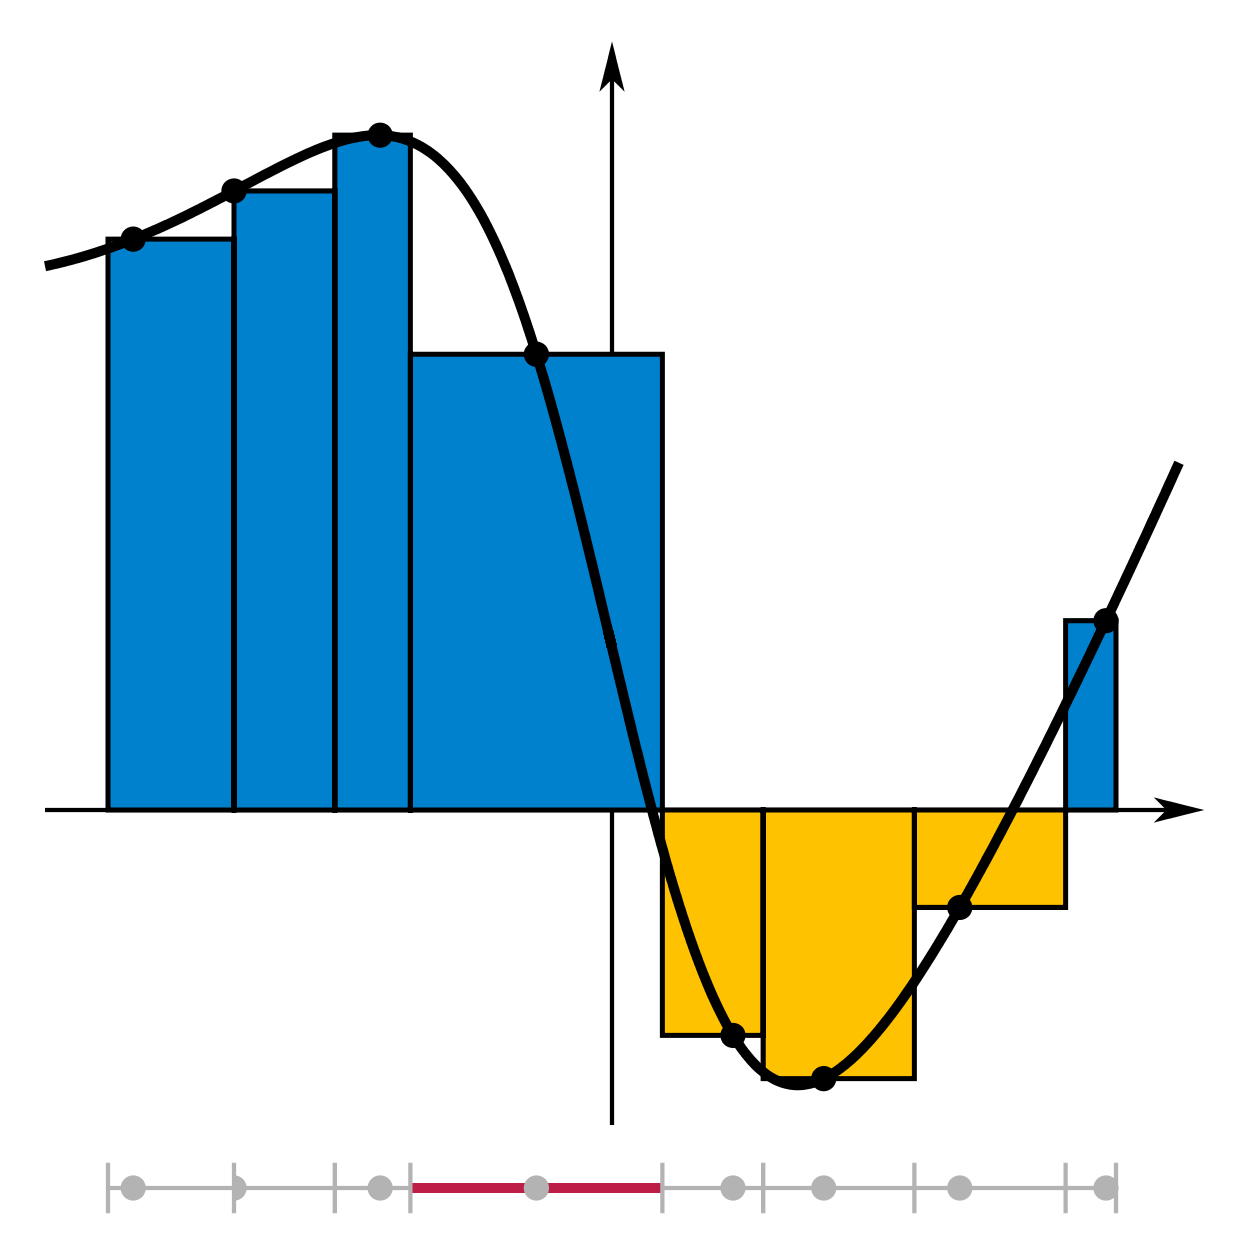
\includegraphics[width=0.4\textwidth]{tu/积分定义4.png}
    \caption*{\texttt{用矩形近似表示函数曲线到$x$轴的面积}}
\end{figure}

\begin{df}{\textbf{区间的分割}}
    \mbox{} \\
    给定闭区间$I=[a; b]$及一列从小到大排列的数$a = x_0 < x_1 < \cdots < x_{n-1} < x_n = b$。
    则把区间$I$分成$n$个子区间$[x_0; x_1], \,\,\, [x_1; x_2], \,\,\,\cdots, \,\,\,[x_{n-1}; x_n]$,就是这一列数对区间的分割。
    我们用数列$(x_0, x_1, \cdots, x_n)$表示这个分割。

    如果区间的分割有$n$个子区间,就说它是区间的$\boldsymbol{n}$\textbf{阶分割}。
    如果区间的分割使得所有子区间长度都不超过某个数$d$,就说它是区间的$\boldsymbol{d}$\textbf{\,–\,分割}。

    设$f$是定义在$I$上的函数。给定区间的某个分割,
    在该分割的各个子区间中取样$c_i\in [x_{i-1}; x_{i}]$,其函数值$f(c_i)$与区间长度的乘积的总和:
    $$ \sum_{i=1}^n (x_i - x_{i-1}) f(c_i) $$
    称为函数关于该分割的\textbf{取样和}。

    如果取样$c_i$是各个区间上函数取最大值的点,就说取样和是函数关于该分割的\textbf{上限和};
    如果取样$c_i$是各个区间上函数取最小值的点,就说取样和是函数关于该分割的\textbf{下限和}。

    显然,下限和小于等于任何取样和,任何取样和小于等于上限和。

\end{df}

给定区间$I$上的函数$f$,如果可以找到区间$I$的某个分割,使得$f$在分割的每个子区间上都是常函数,就说$f$是\textbf{分段常函数},也叫\textbf{阶梯函数}。
显然,阶梯函数背后总有一个分割。如果我们把这个分割的子区间继续拆分,$f$仍然是阶梯函数。

不难发现,阶梯函数的积合,我们可以直接定义为相关矩形的面积之和。具体来说,$f$关于分割$(x_0, x_1, \cdots, x_n)$的积合就是:
$$ \sum_{i=1}^n (x_i - x_{i-1}) f(c_i) $$
其中$c_i$可以是任意取样,因为$f$在子区间上是常函数。

对一般的函数来说,我们可以用阶梯函数来逼近它。对闭区间上连续函数$f$的任何分割,我们考虑两个阶梯函数,
一个在分割的各个子区间上取$f$的最大值,另一个在分割的各个子区间上取$f$的最小值。这两个阶梯函数都可以定义积合,
两者分别对应函数关于该分割的上限和与下限和。

如果我们把分割的子区间继续拆分,这两个积合会怎么变化呢?

\begin{wrapfigure}[8]{l}{0.52\textwidth} 
    \vspace{-32pt}
    \flushleft
    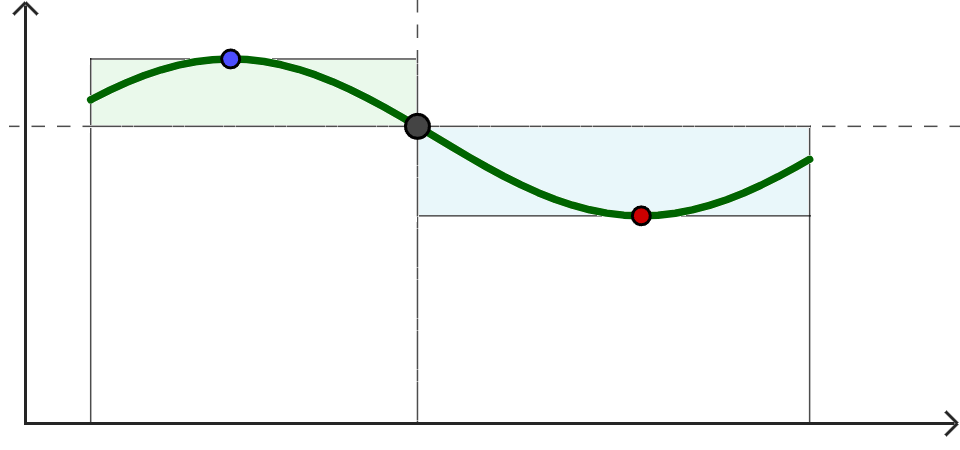
\includegraphics[width=0.5\textwidth]{tu/积分定义2.png}
    \caption*{\texttt{把区间拆成左右两份,最大值不超过原来的最大值(${\color{blue} \bullet}$),最小值不小于原来的最小值(${\color{red} \bullet}$)。}}
\end{wrapfigure}

考虑其中一个子区间,我们把它拆成左右两份,在两边分别取最大值,
两个最大值都不会超过整个子区间的最大值。同理,在两边分别取最小值,两个最小值都不会小于整个子区间的最小值。
因此,拆分后,$f$关于新分割的上限和不增加,下限和不减少。

\begin{wrapfigure}[8]{r}{0.32\textwidth} %this figure will be at the right
    \vspace{-35pt}
    \flushright
    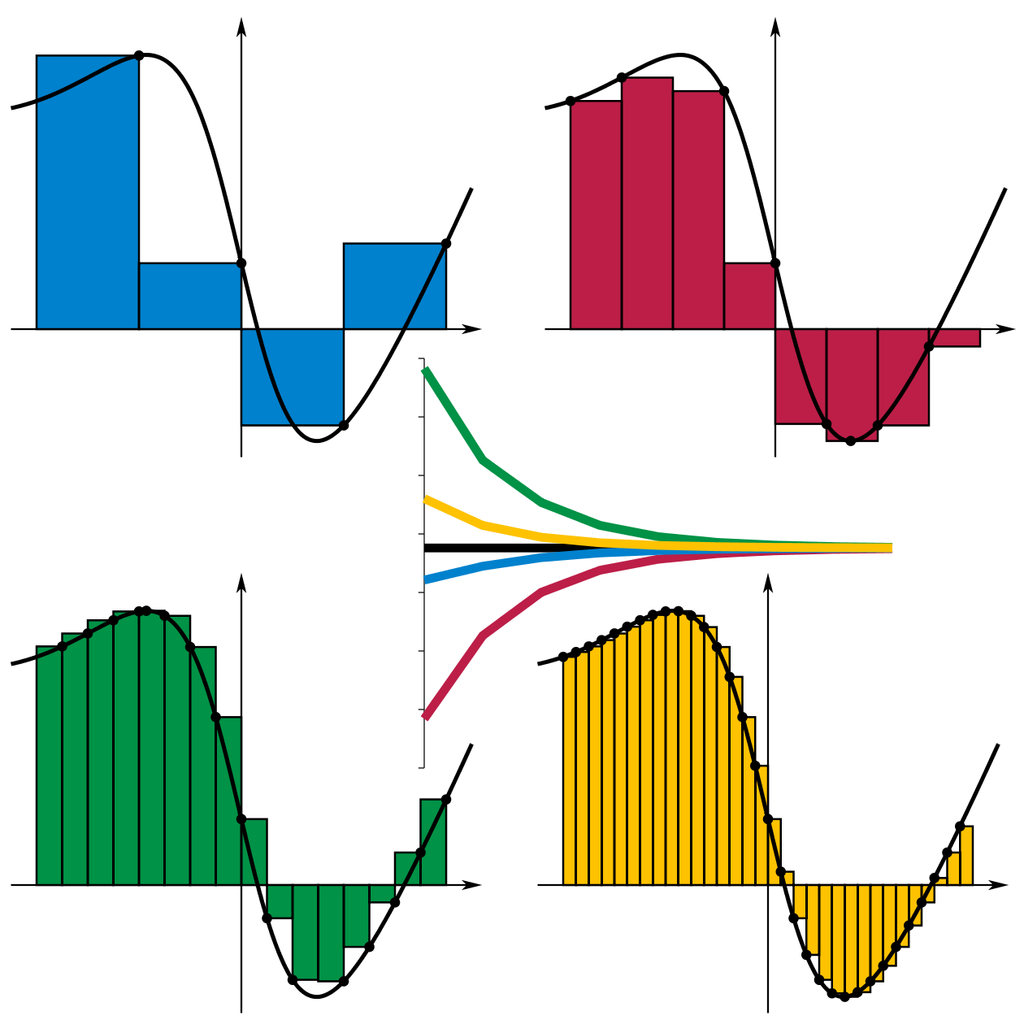
\includegraphics[width=0.3\textwidth]{tu/积分定义6.png}
    \caption*{\texttt{各种分割的取样和,随着分割越来越细,趋于同一个数。}}
\end{wrapfigure}

直觉上,对于一般的函数,分割得越细,
上限和会越来越小,下限和会越来越大;上限和与下限和之间的差距会不断变小。
如果对于任何分割,只要分割越来越细,上下限和之间的差距就越来越小,而且最后都趋于同一个数,
那么这个数就可以看作函数曲线到$x$轴的面积,也就是函数在区间上的积合。

事实上也是这样吗?

为此,我们先说明几个关于上下限和的结论。

把分割的子区间继续拆分,称为\textbf{细化}。给定一个分割,将它的子区间拆分,就是在分割点序列相应的位置插入
新的数。比如把$[x_i; x_{i+1}]$拆分为两个区间$[x_i; y]$和$[y; x_{i+1}]$,就是在$(x_0, x_1, \cdots, x_n)$的$x_i$和$x_{i+1}$之间插入$y$。

因此,两个分割,如果其中一个的分割点集合是另一个的子集,就说后者是前者的\textbf{细化分割}。

上面已经说明,分割细化之后,上限和不变或减小,下限和不变或增大。任意给两个分割,考虑它们的分割点的并集。
这个集合对应的分割同时是两个分割的细化,可以说是两者的共同细化分割。
因此其中一个分割的下限和不大于共同细化分割的下限和,因而不大于共同细化分割的上限和,从又不大于另一个分割的上限和。

这说明区间的任一分割的下限和小于等于任一分割的上限和。
也就是说,如果把$f$在区间上的所有上限和称为集合$S^{\text{上}}$,所有下限和称为集合$S^{\text{下}}$,
那么$S^{\text{下}}$的任何元素小于等于$S^{\text{上}}$的任何元素,
$S^{\text{上}}$的下确界大于等于$S^{\text{下}}$的上确界。

最后证明两者确实相等。

\begin{tm}\label{tm:c-1-10}
    设函数$f$在闭区间$[a; b]$上连续。对任何$r>0$,都可以找到$d>0$,
    使得$f$关于区间的所有$d$\,–\,分割的上下限和之差都小于$r$。
\end{tm}

\begin{proof}
    函数$f$在闭区间$[a; b]$上连续,因此一致连续。也就是说,对任意正数$r$,
    可以找到$d>0$,只要区间中两点$x,y$距离小于等于$d$,就有:
    $$ |f(x) - f(y)| < \frac{r}{b - a}. $$
    对任何的$d$\,–\,分割,按照定义,其任一子区间内两点距离小于等于$d$,因此该子区间的最大值和最小值之差小于$\frac{r}{b - a}$。
    
    把各个子区间上的最大值和最小值之差乘以子区间长度再加起来,
    就是上限和与下限和之差。也就是说:
    $$ \mbox{上限和} - \mbox{下限和} < \sum_{i=0}^n (x_i - x_{i+1}) \cdot \frac{r}{b - a} = (b - a) \cdot \frac{r}{b - a} = r.$$
\end{proof}

定理\ref{tm:c-1-10}说明,可以在$S^{\text{上}}$和$S^{\text{下}}$中分别找一个元素,两者差小于$r$,其中$r$是任意小的正数。
既然如此,$S^{\text{上}}$的下确界和$S^{\text{下}}$的上确界分别小于等于、大于等于这两个元素,
这就说明对任意小的正数$r$,$S^{\text{上}}$的下确界小于$S^{\text{下}}$的上确界加$r$。
因此$S^{\text{上}}$的下确界小于等于$S^{\text{下}}$的上确界。

结合前面的另一个不等关系,就得到结论:
$S^{\text{上}}$的下确界等于$S^{\text{下}}$的上确界。这就是我们要定义的积合。

\begin{sk}
    \mbox{} \\
    \indent 1. 用阶梯函数的面积逼近,是否是构造积合的唯一方法? \\
    \indent 2. 这样定义的积合,是否满足积合作为面积的基本性质?如何证明?\\
    \indent 3. 不连续的函数,能否定义积合?哪些可以?如何定义?\\
    \indent 4. 本节的构造过程是否说明,可以用阶梯函数逼近闭区间上的连续函数?
\end{sk}

\section{常用的积合函数}

下面给出一些常用的显式可积函数的积合。要注意的是,目前我们只定义了闭区间上连续函数的积合。
闭区间上不连续的函数,没有定义积合。

\begin{center}
    \renewcommand{\arraystretch}{2}
    \setlength{\extrarowheight}{-3pt}
    \begin{longtable}{|l|l|}
        \hline \multicolumn{1}{|c|}{\textbf{函数表达式}} & \multicolumn{1}{c|}{\textbf{积合函数}} \\[4pt] 
        \hline    
        $\displaystyle x\mapsto r$ & $\displaystyle \int_a^x f = r(x - a)$ \\[4pt]
        \hline    
        $\displaystyle x\mapsto x^n,\,\,\,n\neq -1$ & $\displaystyle \int_a^x f = \frac{x^{n+1} - a^{n+1}}{n+1}$ \\[4pt]
        \hline    
        $\displaystyle x\mapsto \frac{1}{x}, \,\,\, x > 0$ & $\displaystyle \int_a^x f = \ln{x} - \ln{a}$ \\[4pt]
        \hline    
        $\displaystyle x\mapsto \frac{1}{x}, \,\,\, x < 0$ & $\displaystyle \int_a^x f = \ln{(-x)} - \ln{(-a)}$ \\[4pt]
        \hline
        $\displaystyle x\mapsto r^x,\,\,\, r>0$ & $\displaystyle \int_a^x f = \frac{r^x - r^a}{\ln{r}}$ \\[4pt]
        \hline
        $\displaystyle x\mapsto e^x$ & $\displaystyle \int_a^x f = e^x - e^a$ \\[4pt]
        \hline    
        $\displaystyle x\mapsto xe^x$ & $\displaystyle \int_a^x f = (x - 1)e^x - (a - 1)e^a$ \\[4pt]
        \hline
        $\displaystyle x\mapsto \ln{x}$ & $\displaystyle \int_a^x f = x\ln{x} - x - a\ln{a} + a$ \\[4pt]
        \hline
        $\displaystyle x\mapsto \frac{1}{x\ln{x}},\,\,\, x>1$ & $\displaystyle \int_a^x f = \ln{(\ln{x})} - \ln{(\ln{a})}$ \\[4pt]
        \hline
        $\displaystyle x\mapsto \frac{1}{x\ln{x}},\,\,\, x<1$ & $\displaystyle \int_a^x f = \ln{(-\ln{x})} - \ln{(-\ln{a})}$ \\[4pt]
        \hline    
        $\displaystyle x\mapsto \sin{x}$ & $\displaystyle \int_a^x f = \cos{a} - \cos{x}$ \\[4pt]
        \hline    
        $\displaystyle x\mapsto \cos{x}$ & $\displaystyle \int_a^x f = \sin{x} - \sin{a}$ \\[4pt]
        \hline    
        $\displaystyle x\mapsto \tan{x}$ & $\displaystyle \int_a^x f = \ln{|\cos{a}|} - \ln{|\cos{x}|}$ \\[4pt]
        \hline    
        $\displaystyle x\mapsto \cot{x}$ & $\displaystyle \int_a^x f = \ln{|\sin{x}|} - \ln{|\sin{a}|}$ \\[4pt]
        \hline    
        $\displaystyle x\mapsto \csc{x}$ & $\displaystyle \int_a^x f = \ln{\left|\tan{\left(\frac{x}{2}\right)}\right|} - \ln{\left|\tan{\left(\frac{a}{2}\right)}\right|}$ \\[4pt]
        \hline    
        $\displaystyle x\mapsto \sec{x}$ & $\displaystyle \int_a^x f = \ln{\left|\tan{\left(\frac{x}{2} + \frac{\pi}{4}\right)}\right|} - \ln{\left|\tan{\left(\frac{a}{2} + \frac{\pi}{4}\right)}\right|}$ \\[4pt]
        \hline    
        $\displaystyle x\mapsto \sec^2{x}$ & $\displaystyle \int_a^x f = \tan{x} - \tan{a}$ \\[4pt]
        \hline    
        $\displaystyle x\mapsto \csc^2{x}$ & $\displaystyle \int_a^x f = \cot{a} - \cot{x}$ \\[4pt]
        \hline    
        $\displaystyle x\mapsto \frac{\sin{x}}{\cos^2{x}}$ & $\displaystyle \int_a^x f = \sec{x} - \sec{a}$ \\[4pt]
        \hline    
        $\displaystyle x\mapsto \frac{\cos{x}}{\sin^2{x}}$ & $\displaystyle \int_a^x f = \csc{a} - \csc{x}$ \\[4pt]
        \hline    
        $\displaystyle x\mapsto \frac{1}{x^2 + 1}$ & $\displaystyle \int_a^x f = \arctan{x} - \arctan{a}$ \\[4pt]
        \hline    
        $\displaystyle x\mapsto \frac{1}{\sqrt{1 - x^2}}$ & $\displaystyle \int_a^x f = \arcsin{x} - \arcsin{a}$ \\[4pt]
        \hline    
        $\displaystyle x\mapsto \frac{1}{\sqrt{x^2 - 1}}$ & $\displaystyle \int_a^x f = \ln{\left(x + \sqrt{x^2 - 1}\right)} - \ln{\left(a + \sqrt{a^2 - 1}\right)}$ \\[4pt]
        \hline    
        $\displaystyle x\mapsto \frac{1}{\sqrt{1 + x^2}}$ & $\displaystyle \int_a^x f = \ln{\left(x + \sqrt{1 + x^2}\right)} - \ln{\left(a + \sqrt{1 + a^2}\right)}$ \\[4pt]
        \hline    
        $\displaystyle x\mapsto \sqrt{r^2 - x^2}$ & $\displaystyle \int_a^x f = \frac{1}{2}\left(x\sqrt{r^2 - x^2} + r^2\arcsin{\frac{x}{r}} - a\sqrt{r^2 - a^2} + r^2\arcsin{\frac{a}{r}}\right)$ \\[4pt]
        \hline
    \end{longtable}
\end{center}

\section{积合与函数}

\begin{tm}{\textbf{积合中值定理}}
    如果函数$f$在闭区间$[a; b]$上连续,那么可以找到$c\in[a;b]$使得:
    $$ \int_a^b f = (b - a)\cdot f(c).$$
\end{tm}

\begin{proof}
    考虑$f$在区间上的积合函数:$F: x\mapsto \int_a^x f$。则$f$是$F$的微变函数。
    于是$F$是可微函数,因此根据微变中值定理,可以找到$c\in[a;b]$使得:
    $$ \partial F(c) = \frac{F(b) - F(a)}{b - a}.$$
    根据微积互反定理,$F(b) - F(a) = \int_a^b f$,$\partial F = f$,于是上式变成:
    $$ \int_a^b f = (b - a)\cdot f(c).$$
\end{proof}


\begin{tm}{\textbf{积合余项的微变展开定理}}
    如果函数$f$在包含实数$a$的区间$I$中$n+1$次可微,且$n+1$次微变函数连续,那么对$I$中另一点$x$有:
    \begin{align*}
        f(x) &= f(a) + \sum_{i=1}^n \frac{\partial^i f(a)}{i!} (x - a)^i + \int_a^x \frac{(x - t)^{n}}{n!} \partial^{n+1} f(t)\mathrm{d}t. \\
        &= P_n + Y_n 
    \end{align*}
    其中$Y_n = \int_a^x \frac{(x - t)^{n}}{n!} \partial^{n+1} f(t)\mathrm{d}t$称为局部展开的$n$次积合余项。
\end{tm}

\begin{proof}
    根据微积互反定理,
    $$ f(x) = f(a) + \int_a^x \partial f .$$
    考虑$G : t \mapsto x - t $,$\partial G = -1$。于是:
    $$ \partial (G\cdot \partial f) = -1 \cdot \partial f + G \cdot \partial^2 f. $$
    两边求积合,就得到:
    $$ G(x) \partial f(x) - G(a) \partial f(a) = - \int_a^x \partial f + \int_a^x G \cdot \partial^2 f. $$
    $G(x) = 0$,因此上式变为:
    \begin{align*}
        \int_a^x \partial f &=  G(a) \partial f(a) + \int_a^x G \cdot \partial^2 f \\
        &= (x - a) \partial f(a) + \int_a^b (x - t) \cdot \partial^2 f(t)\mathrm{d}t. 
    \end{align*}
    
    给定正整数$1\leqslant i \leqslant n$,我们希望把$\int_a^x \frac{(x - t)^{(i-1)}}{(i-1)!} \partial^{i} f(t)\mathrm{d}t$
    用$\int_a^x \frac{(x - t)^{i}}{i!} \partial^{i+1} f(t)\mathrm{d}t$表示。

    可以仿照上面的方法。我们考虑$G_i: x\mapsto \frac{(x - t)^i}{i!}$,$\partial G_i(t) = -\frac{(x - t)^{i-1}}{(i-1)!}$,
    因此
    $$ \partial (G\cdot \partial^i f) = -\frac{(x - t)^{i-1}}{(i-1)!} \cdot \partial^i f + G \cdot \partial^{i+1} f. $$
    两边求积合,就得到:
    $$ G(x) \partial^i f(x) - G(a) \partial^i f(a) = - \int_a^x \frac{(x - t)^{i-1}}{(i-1)!} \partial^i f + \int_a^x G \cdot \partial^{i+1} f. $$
    $G(x) = 0$,因此上式变为:
    \begin{align*}
        \int_a^x \frac{(x - t)^{i-1}}{(i-1)!}\partial^i f & = G(a) \partial^i f(a)  + \int_a^x G \cdot \partial^{i+1} f \\
        & = \frac{(x - a)^i}{i!} \partial f(a) + \int_a^b \frac{(x - t)^i}{i!}\cdot \partial^{i+1} f(t)\mathrm{d}t
    \end{align*}
    因此,
    \begin{align*}
        f(x) &= f(a) + \int_a^x \partial f(t) \mathrm{d}t \\
        &= f(a) + (x - a) \partial f(a) + \int_a^b (x - t) \cdot \partial^2 f(t) \mathrm{d}t \\
        &= f(a) + (x - a) \partial f(a) + \frac{(x - a)^2}{2} \partial^2 f(a) + \int_a^b \frac{(x - t)^2}{2} \cdot \partial^3 f(t) \mathrm{d}t\\
        & \qquad \qquad \qquad \qquad\qquad \qquad \vdots \\
        &= f(a) + \sum_{i=1}^n \frac{\partial^i f(a)}{i!} (x - a)^i + \int_a^x \frac{(x - t)^{n}}{n!} \partial^{n+1} f(t)\mathrm{d}t. \\
    \end{align*}    
\end{proof}

\begin{sk}
    \mbox{} \\
    \indent 1. 积合余项的微变展开定理的证明用了什么积分技巧?\\
    \indent 2. 不用微变中值定理,能否证明积合中值定理?\\
    \indent 3. 从本节证明的两个定理出发,能否证明微变余项的微变展开定理?能否证明局部展开定理?
\end{sk}

\chapter{平直空间}

\begin{tm}\label{tm:d-1-20}
    设有不全为零的一组向量$\mathbf{v}_1, \mathbf{v}_2 , \cdots , \mathbf{v}_m$直相关。不妨设$\mathbf{v}_1 \neq 0$,那么存在下标$j \in \{2,3, \cdots, m\}$满足以下性质:
    \begin{enumerate}
    \item $\mathbf{v}_j \in \langle \mathbf{v}_1, \mathbf{v}_2 , \cdots , \mathbf{v}_{j-1}\rangle$
    \item 如果从$\mathbf{v}_1, \mathbf{v}_2 , \cdots , \mathbf{v}_m$中移除$\mathbf{v}_j$,剩余向量生成的空间与原来$m$个向量生成的空间相同。
    \end{enumerate}
\end{tm}

\begin{proof}
    按直相关的定义,存在不全为零的标量系数$a_1, a_2, \cdots, a_m$使得:
    $$ a_1\mathbf{v}_1+a_2\mathbf{v}_2+\cdots+a_m\mathbf{v}_m = \mathbf{0}. $$
    由于$\mathbf{v}_1 \neq 0$,所以$a_2, \cdots, a_m$不全为0. 否则可推出$a_1\mathbf{v}_1 = \mathbf{0}$,从而$a_1$也是0,矛盾。\\
    假设$j$是$a_2, \cdots, a_m$中不为0的数的下标中最大的那个,也就是说$\forall k > j, a_k = 0$. 这表示$ a_1\mathbf{v}_1+a_2\mathbf{v}_2+\cdots+a_j\mathbf{v}_j = \mathbf{0}. $
    所以
    $$ \mathbf{v}_j = -\frac{a_1}{a_j}\mathbf{v}_1-\frac{a_2}{a_j}\mathbf{v}_2-\cdots-\frac{a_{j-1}}{a_j}\mathbf{v}_{j-1} \in \langle \mathbf{v}_1, \mathbf{v}_2 , \cdots , \mathbf{v}_{j-1}\rangle. $$
    由于$ \mathbf{v}_j$可以表示为$\mathbf{v}_1, \mathbf{v}_2 , \cdots , \mathbf{v}_{j-1}$的直组合,设某个向量是$\mathbf{v}_1, \mathbf{v}_2 , \cdots , \mathbf{v}_m$的直组合:
    $$ \mathbf{u} = b_1\mathbf{v}_1+b_2\mathbf{v}_2+\cdots+b_m\mathbf{v}_m$$
    把右侧表达式中的$\mathbf{v}_j$替换为$\mathbf{v}_1, \mathbf{v}_2 , \cdots , \mathbf{v}_{j-1}$的直组合,就得到了不含$\mathbf{v}_j$的直组合表达式。\\
    所以,去除$\mathbf{v}_j$,整组向量的生成空间不变\footnote{其实我们只证明了一个方向的归属关系,不过另一个方向比较显然,留给读者思考。}。\\
\end{proof}

\begin{tm}\label{tm:d-1-30}
    有限生成空间中,任何一族直无关的向量,向量的个数都不多于任意一个生成族的向量个数。
\end{tm}

\begin{proof}
    
    设$\mathfrak{F}_{\mathbf{u}} = (\mathbf{u}_1, \mathbf{u}_2, \cdots , \mathbf{u}_n )$是平直空间$\mathbb{V}$中一组直无关的向量,
    $\mathfrak{F}_{\mathbf{v}} = (\mathbf{v}_1, \mathbf{v}_2, \cdots , \mathbf{v}_m )$是$\mathbb{V}$的生成族。
    我们要证明$n \leq m$. 

    我们把$\mathfrak{F}_{\mathbf{v}}$中的元素逐一替换成$\mathfrak{F}_{\mathbf{u}}$中元素,一共替换$n$次。
    如果以上步骤能完成,说明$\mathfrak{F}_{\mathbf{v}}$的长度不少于$n$,就完成了证明。

    第一步替换具体操作为:

    将$\mathbf{u}_1$添加到$(\mathbf{v}_1, \mathbf{v}_2, \cdots , \mathbf{v}_m )$左侧,形成
    $$\mathfrak{F}_{\mathbf{v}}^{(1)} = (\mathbf{u}_1, \mathbf{v}_1, \mathbf{v}_2, \cdots , \mathbf{v}_m ).$$
    由于$\mathfrak{F}_{\mathbf{v}}$是$\mathbb{V}$的生成族,$\mathbf{u}_1$可以表示为$\mathbf{v}_1, \mathbf{v}_2, \cdots , \mathbf{v}_m$的直组合。
    即$\mathfrak{F}_{\mathbf{v}}^{(1)}$是直相关的。所以根据定理\ref{tm:d-1-20},
    我们可以去掉某个$\mathbf{v}$,使得其生成空间不变(仍然为$\mathbb{V}$).
    这样$\mathfrak{F}_{\mathbf{v}}^{(1)}$变为一组元素个数为$m$的向量,并且仍然是$\mathbb{V}$的生成族。
    
    此后第$j$步,具体操作为:

    将$\mathbf{u}_j$添加到$\mathfrak{F}_{\mathbf{v}}^{(j-1)}$中$\mathbf{u}_{j-1}$的右侧。
    注意到$\mathfrak{F}_{\mathbf{v}}^{(j-1)}$是由左侧的$\mathbf{u}_1, \mathbf{u}_2, \cdots , \mathbf{u}_{j-1}$
    和右侧的$\mathfrak{F}_{\mathbf{v}}$中元素拼接而成,
    所以$\mathbf{u}_j$被放置在$\mathfrak{F}_{\mathbf{v}}^{(j-1)}$中原属于$\mathfrak{F}_{\mathbf{u}}$的元素
    和原属于$\mathfrak{F}_{\mathbf{v}}$的元素的分界上。
    放置之后形成的$\mathfrak{F}_{\mathbf{v}}^{(j)}$,“布局”和$\mathfrak{F}_{\mathbf{v}}^{(j-1)}$一样,
    仍然是由左侧原属于$\mathfrak{F}_{\mathbf{}}$的元素和右侧原属于$\mathfrak{F}_{\mathbf{v}}$的元素构成。
    
    这时,通过和第一步同样的逻辑,我们知道$\mathfrak{F}_{\mathbf{v}}^{(j)}$是直相关的,所以根据定理\ref{tm:d-1-20},
    可以从中找到某个元素:它属于它之前的元素的生成空间,
    并且去除这个元素后,$\mathfrak{F}_{\mathbf{v}}^{(j)}$生成的空间不变,仍然是$\mathbb{V}$。

    注意由于$\mathfrak{F}_{\mathbf{u}}$是直无关的,我们找到的这个元素,
    肯定不会是左侧原属于$\mathfrak{F}_{\mathbf{u}}$的元素,
    因而只能是原属于$\mathfrak{F}_{\mathbf{v}}$的元素。

    这样,每一步操作,我们都加入一个原属于$\mathfrak{F}_{\mathbf{u}}$的元素,去除一个原属于$\mathfrak{F}_{\mathbf{v}}$的元素。
    元素个数不变,且最后形成的向量组仍然是$\mathbb{V}$的生成集。

    那么,是否会在某一步操作时,发现已经没有原属于$\mathfrak{F}_{\mathbf{v}}$的元素可以去除呢?

    如果这种情况发生,说明加入一个原属于$\mathfrak{F}_{\mathbf{u}}$的元素后,
    只有原属于$\mathfrak{F}_{\mathbf{u}}$的元素了。
    这时候向量组一方面仍然是直相关的,但同时元素全是$\mathfrak{F}_{\mathbf{u}}$中元素。
    说明$\mathfrak{F}_{\mathbf{u}}$也是直相关的。矛盾!

    所以每一步操作都可以完整进行,直到$\mathfrak{F}_{\mathbf{u}}$中所有元素放入完毕。
    这样,我们就证明了$\mathfrak{F}_{\mathbf{v}}$的长度不少于$n$,即$n \leq m$.
\end{proof}

\begin{tm}\label{tm:d-1-40}
    可以通过适当地移除元素,把有限生成空间$\mathbb{V}$的每个生成族变成基底。
\end{tm}

\begin{proof}
    设$\mathcal{F}_{\mathbf{v}} = (\mathbf{v}_1, \mathbf{v}_2, \cdots , \mathbf{v}_m )$是$\mathbb{V}$的生成族。
    
    如果$\mathcal{F}_{\mathbf{v}}$直无关,则按照定义,$\mathcal{F}_{\mathbf{v}}$是一组基。

    如果$\mathcal{F}_{\mathbf{v}}$直相关。我们进行如下操作:

    首先移除$\mathcal{F}_{\mathbf{v}}$中所有的零向量。
    如果$\mathcal{F}_{\mathbf{v}}$完全由零向量构成,说明$\mathbb{V} = \{\mathbf{0}\}$。
    这时,$\mathcal{F}_{\mathbf{v}}$移除全部元素后剩下空集,直无关且生成$\mathbb{V}$。

    如果$\mathcal{F}_{\mathbf{v}}$中还有若干非零向量,且仍直相关,
    根据定理\ref{tm:d-1-20},可以从其中找出一个向量,把它从$\mathcal{F}_{\mathbf{v}}$移除后,
    生成空间不变,$\mathcal{F}_{\mathbf{v}}$仍旧是生成族。

    如果$\mathcal{F}_{\mathbf{v}}$仍然直相关,则重复以上操作。
    每次操作后,$\mathcal{F}_{\mathbf{v}}$中元素数量减少$1$。
    所以,有限次操作之后,$\mathcal{F}_{\mathbf{v}}$变为直无关的生成族。
    这时我们就得到了空间的基底。

\end{proof}

从上面的定理可以推出:
\begin{tm}\label{tm:d-1-50}
    任意有限生成空间都有基底。
\end{tm}

空间的任意生成集都可以缩减为它的基底。那么任意直无关的向量能否扩充为基底呢?
\begin{tm}\label{tm:d-1-60}
    可以通过适当地添加元素,把有限生成空间$\mathbb{V}$的每一组直无关的向量变成基底。
\end{tm}

\begin{proof}
    设$\mathcal{F}_{\mathbf{v}} = (\mathbf{v}_1, \mathbf{v}_2, \cdots , \mathbf{v}_m )$是$\mathbb{V}$中一组直无关的向量。

    如果$\mathcal{F}_{\mathbf{v}}$生成$\mathbb{V}$,则按照定义,$\mathcal{F}_{\mathbf{v}}$是一组基。

    如果$\mathcal{F}_{\mathbf{v}}$生成的空间不是$\mathbb{V}$,则是$\mathbb{V}$的真子空间。

    空间$\mathbb{V}$是有限生成空间,所以存在生成族:$\mathcal{F}_{\mathbf{u}} = (\mathbf{u}_1, \mathbf{u}_2, \cdots , \mathbf{u}_n )$. 我们进行以下操作:

    逐个查看$(\mathbf{u}_1, \mathbf{u}_2, \cdots , \mathbf{u}_n )$,其中必然有一个元素不在$\langle\mathcal{F}_{\mathbf{v}}\rangle$中。

    这是因为,反设$\mathcal{F}_{\mathbf{u}}$中每个元素都能写成$\mathcal{F}_{\mathbf{v}}$中元素的直组合,
    那么由于$\mathbb{V}$中任一元素都能写成$\mathcal{F}_{\mathbf{u}}$中元素的直组合,
    从而也能写成$\mathcal{F}_{\mathbf{v}}$中元素的直组合。
    这说明$\mathcal{F}_{\mathbf{v}}$可以生成整个空间,矛盾!

    所以,必然存在某个$\mathbf{u}_i$不在$\langle\mathcal{F}_{\mathbf{v}}\rangle$中。
    我们将它添加到$\mathcal{F}_{\mathbf{v}}$里去,得到的仍然是一组直无关的向量。

    每次操作,$\mathcal{F}_{\mathbf{v}}$中增加一个元素。所以,要么在有限次操作后,$\langle\mathcal{F}_{\mathbf{v}}\rangle = \mathbb{V}$,
    我们得到$\mathbb{V}$的直无关的生成集(也就是基底);
    要么$\mathcal{F}_{\mathbf{v}}$中元素个数超过$n$,而这和定理\ref{tm:d-1-30}矛盾。

\end{proof}

我们甚至有更具体的结论:
\begin{tm}\label{tm:d-1-70}
    给定有限生成空间$\mathbb{V}$的子空间$\mathbb{U}$,存在另一个子空间$\mathbb{W}$,使得
    $$ \mathbb{V} = \mathbb{U} + \mathbb{W}.$$
    且$\mathbb{U} \cap \mathbb{W} = \{\mathbf{0}\}$
    $\mathbb{W}$称为子空间$\mathbb{U}$的\textbf{补空间},一般记作$\mathbb{U}^c.$
\end{tm}

\begin{proof}
    设$\mathcal{B}_1$是子空间$\mathbb{U}$的基底。$\mathcal{B}_1$是直无关的。
    所以可以通过适当添加元素,将$\mathcal{B}_1$扩充为$\mathbb{V}$的基底$\mathcal{B}$。

    设$\mathcal{B}_2$是$\mathcal{B}_1$扩充到$\mathcal{B}$过程中添加的所有元素。
    $\mathcal{B}_2$也是直无关的。考虑$\mathbb{W} = \langle\mathcal{B}_2\rangle$,可以验证:
    $$ \mathbb{V} = \mathbb{U} + \mathbb{W}.$$

    下面证明$ \mathbb{U} \cap \mathbb{W} = \{\mathbf{0}\}$。

    设$\mathcal{B}_1 = (\mathbf{v}_1, \mathbf{v}_2, \cdots , \mathbf{v}_m )$,
    $\mathcal{B}_2 = (\mathbf{v}_{m+1}, \cdots , \mathbf{v}_n )$。 
    设$ \mathbf{u} \in \mathbb{U} \cap \mathbb{W}$,则:
    $$ \mathbf{u} = a_1\mathbf{v}_1 + a_2\mathbf{v}_2 + \cdots + a_m\mathbf{v}_m = a_{m+1}\mathbf{v}_{m+1} + \cdots + a_n\mathbf{v}_n. $$
    即:
    $$a_1\mathbf{v}_1 + a_2\mathbf{v}_2 + \cdots + a_m\mathbf{v}_m + (-a_{m+1})\mathbf{v}_{m+1} + \cdots + (-a_{n})\mathbf{v}_{n} = \mathbf{0}. $$
    然而$(\mathbf{v}_1, \mathbf{v}_2, \cdots , \mathbf{v}_n )$是直无关的。所以,
    $$ a_1 = a_2 = \cdots = a_m = -a_{m+1} = \cdots = -a_n = 0.$$
    所以$\mathbf{u} = \mathbf{0}$。
    因此,$ \mathbb{U} \cap \mathbb{W} = \{\mathbf{0}\}$.

\end{proof}

关于子空间交集与和空间维数的定理:
\begin{tm}{\textbf{维数基本定理}}\label{tm:d-1-80}
    设$\mathbb{U}$和$\mathbb{W}$是有限维空间$\mathbb{V}$的两个子空间,则它们的维数满足以下关系:
    $$ \dim (\mathbb{U} + \mathbb{W}) = \dim \mathbb{U} + \dim \mathbb{W} - \dim (\mathbb{U} \cap \mathbb{W}).$$
\end{tm}

\begin{proof}
    记$\mathbb{T} = \mathbb{U} \cap \mathbb{W}$. 根据定理 \ref{tm:d-1-70},
    我们可以给$\mathbb{T}$在$\mathbb{U}$和$\mathbb{W}$里各自找一个补空间:
    $$ \mathbb{U} = \mathbb{T} \oplus \mathbb{U}', \,\,\, \mathbb{W} = \mathbb{T} \oplus \mathbb{W}'.$$
    记$\dim \mathbb{T} = h, \,\,\, \dim \mathbb{U}' = f, \,\,\, \dim \mathbb{W}' = g$。
    我们考虑这三个空间的基:
    $$ \mathcal{B}_T = (\mathbf{t}_1, \mathbf{t}_2, \cdots, \mathbf{t}_h), \,\,\, \mathcal{B}_{U'} = (\mathbf{u}_1, \mathbf{u}_2, \cdots, \mathbf{u}_f), \,\,\, \mathcal{B}_{W'} = (\mathbf{w}_1, \mathbf{w}_2, \cdots, \mathbf{w}_g). $$  
    其中$\mathcal{B}_{U'}$和$\mathcal{B}_{W'}$分别是$\mathbb{T}$按照定理 
    \ref{tm:d-1-70}证明中的方式扩充为$\mathbb{U}$和$\mathbb{W}$时得到的向量族。
    这表示,$\mathcal{B}_T\cup\mathcal{B}_{U'}$是$\mathbb{U}$的基,
    $\mathcal{B}_T\cup\mathcal{B}_{W'}$是$\mathbb{W}$的基。
    所以,
    $$\dim \mathbb{U} = h + f,\,\,\,\dim \mathbb{W} = h + g.$$
    只需证明:$ \dim (\mathbb{U} + \mathbb{W}) = h + f + g.$

    为此我们证明$\mathcal{B}_T\cup\mathcal{B}_{U'}\cup\mathcal{B}_{W'}$是$\mathbb{U} + \mathbb{W}$的一组基。

    首先,$\mathcal{B}_T\cup\mathcal{B}_{U'}\cup\mathcal{B}_{W'}$可以生成$\mathbb{U}$,
    也可以生成$\mathbb{W}$,所以可以生成$\mathbb{U} + \mathbb{W}$。

    其次,证明$\mathcal{B}_T\cup\mathcal{B}_{U'}\cup\mathcal{B}_{W'}$直无关。

    假设零向量可以分解为$\mathcal{B}_T\cup\mathcal{B}_{U'}\cup\mathcal{B}_{W'}$的直组合,
    则说明零向量可以表示为:
    $$ \mathbf{0} = \mathbf{t} + \mathbf{u} + \mathbf{w}. \,\,\,\mathbf{t}\in\mathbb{T},\,\,\mathbf{u}\in\mathbb{U}',\,\,\mathbf{w}\in\mathbb{W}'.$$
    所以$\mathbf{u} = -\mathbf{t} - \mathbf{w} \in \mathbb{W}$.
    也就是说,$\mathbf{u}\in \mathbb{U}'\cap\mathbb{W}$。

    然而$\mathbb{U}'\cap\mathbb{W} \subset \mathbb{U}\cap\mathbb{W} = \mathbb{T}$,
    所以$\mathbf{u}\in\mathbb{T}\cap\mathbb{U}' = \{\mathbf{0}\}$。

    因此,$\mathbf{u} = \mathbf{0}.$

    同理可得,$\mathbf{w} = \mathbf{0}.$ 所以$\mathbf{t} = \mathbf{0}.$

    而$\mathcal{B}_T$、$\mathcal{B}_{U'}$和$\mathcal{B}_{W'}$分别是直无关的。
    所以零向量分解为$\mathcal{B}_T\cup\mathcal{B}_{U'}\cup\mathcal{B}_{W'}$的直组合时,
    每个分量系数都是0. 
    这就证明$\mathcal{B}_T\cup\mathcal{B}_{U'}\cup\mathcal{B}_{W'}$直无关,
    从而是$\mathbb{U} + \mathbb{W}$的一组基。

\end{proof}

从这个定理可以看出子空间和集合的相似之处。

% \begin{sk}
%     \mbox{} \\
%     \indent 1. 总结平直空间各个概念和集合的相似之处。\\
% \end{sk}

\end{appendix}


\end{document}
